\documentclass[]{book}
\usepackage{lmodern}
\usepackage{amssymb,amsmath}
\usepackage{ifxetex,ifluatex}
\usepackage{fixltx2e} % provides \textsubscript
\ifnum 0\ifxetex 1\fi\ifluatex 1\fi=0 % if pdftex
  \usepackage[T1]{fontenc}
  \usepackage[utf8]{inputenc}
\else % if luatex or xelatex
  \ifxetex
    \usepackage{mathspec}
  \else
    \usepackage{fontspec}
  \fi
  \defaultfontfeatures{Ligatures=TeX,Scale=MatchLowercase}
\fi
% use upquote if available, for straight quotes in verbatim environments
\IfFileExists{upquote.sty}{\usepackage{upquote}}{}
% use microtype if available
\IfFileExists{microtype.sty}{%
\usepackage{microtype}
\UseMicrotypeSet[protrusion]{basicmath} % disable protrusion for tt fonts
}{}
\usepackage[margin=1in]{geometry}
\usepackage{hyperref}
\hypersetup{unicode=true,
            pdftitle={Statistical Analysis and Visualizations Using R},
            pdfauthor={Okan Bulut},
            pdfborder={0 0 0},
            breaklinks=true}
\urlstyle{same}  % don't use monospace font for urls
\usepackage{natbib}
\bibliographystyle{apalike}
\usepackage{color}
\usepackage{fancyvrb}
\newcommand{\VerbBar}{|}
\newcommand{\VERB}{\Verb[commandchars=\\\{\}]}
\DefineVerbatimEnvironment{Highlighting}{Verbatim}{commandchars=\\\{\}}
% Add ',fontsize=\small' for more characters per line
\usepackage{framed}
\definecolor{shadecolor}{RGB}{248,248,248}
\newenvironment{Shaded}{\begin{snugshade}}{\end{snugshade}}
\newcommand{\AlertTok}[1]{\textcolor[rgb]{0.94,0.16,0.16}{#1}}
\newcommand{\AnnotationTok}[1]{\textcolor[rgb]{0.56,0.35,0.01}{\textbf{\textit{#1}}}}
\newcommand{\AttributeTok}[1]{\textcolor[rgb]{0.77,0.63,0.00}{#1}}
\newcommand{\BaseNTok}[1]{\textcolor[rgb]{0.00,0.00,0.81}{#1}}
\newcommand{\BuiltInTok}[1]{#1}
\newcommand{\CharTok}[1]{\textcolor[rgb]{0.31,0.60,0.02}{#1}}
\newcommand{\CommentTok}[1]{\textcolor[rgb]{0.56,0.35,0.01}{\textit{#1}}}
\newcommand{\CommentVarTok}[1]{\textcolor[rgb]{0.56,0.35,0.01}{\textbf{\textit{#1}}}}
\newcommand{\ConstantTok}[1]{\textcolor[rgb]{0.00,0.00,0.00}{#1}}
\newcommand{\ControlFlowTok}[1]{\textcolor[rgb]{0.13,0.29,0.53}{\textbf{#1}}}
\newcommand{\DataTypeTok}[1]{\textcolor[rgb]{0.13,0.29,0.53}{#1}}
\newcommand{\DecValTok}[1]{\textcolor[rgb]{0.00,0.00,0.81}{#1}}
\newcommand{\DocumentationTok}[1]{\textcolor[rgb]{0.56,0.35,0.01}{\textbf{\textit{#1}}}}
\newcommand{\ErrorTok}[1]{\textcolor[rgb]{0.64,0.00,0.00}{\textbf{#1}}}
\newcommand{\ExtensionTok}[1]{#1}
\newcommand{\FloatTok}[1]{\textcolor[rgb]{0.00,0.00,0.81}{#1}}
\newcommand{\FunctionTok}[1]{\textcolor[rgb]{0.00,0.00,0.00}{#1}}
\newcommand{\ImportTok}[1]{#1}
\newcommand{\InformationTok}[1]{\textcolor[rgb]{0.56,0.35,0.01}{\textbf{\textit{#1}}}}
\newcommand{\KeywordTok}[1]{\textcolor[rgb]{0.13,0.29,0.53}{\textbf{#1}}}
\newcommand{\NormalTok}[1]{#1}
\newcommand{\OperatorTok}[1]{\textcolor[rgb]{0.81,0.36,0.00}{\textbf{#1}}}
\newcommand{\OtherTok}[1]{\textcolor[rgb]{0.56,0.35,0.01}{#1}}
\newcommand{\PreprocessorTok}[1]{\textcolor[rgb]{0.56,0.35,0.01}{\textit{#1}}}
\newcommand{\RegionMarkerTok}[1]{#1}
\newcommand{\SpecialCharTok}[1]{\textcolor[rgb]{0.00,0.00,0.00}{#1}}
\newcommand{\SpecialStringTok}[1]{\textcolor[rgb]{0.31,0.60,0.02}{#1}}
\newcommand{\StringTok}[1]{\textcolor[rgb]{0.31,0.60,0.02}{#1}}
\newcommand{\VariableTok}[1]{\textcolor[rgb]{0.00,0.00,0.00}{#1}}
\newcommand{\VerbatimStringTok}[1]{\textcolor[rgb]{0.31,0.60,0.02}{#1}}
\newcommand{\WarningTok}[1]{\textcolor[rgb]{0.56,0.35,0.01}{\textbf{\textit{#1}}}}
\usepackage{longtable,booktabs}
\usepackage{graphicx,grffile}
\makeatletter
\def\maxwidth{\ifdim\Gin@nat@width>\linewidth\linewidth\else\Gin@nat@width\fi}
\def\maxheight{\ifdim\Gin@nat@height>\textheight\textheight\else\Gin@nat@height\fi}
\makeatother
% Scale images if necessary, so that they will not overflow the page
% margins by default, and it is still possible to overwrite the defaults
% using explicit options in \includegraphics[width, height, ...]{}
\setkeys{Gin}{width=\maxwidth,height=\maxheight,keepaspectratio}
\IfFileExists{parskip.sty}{%
\usepackage{parskip}
}{% else
\setlength{\parindent}{0pt}
\setlength{\parskip}{6pt plus 2pt minus 1pt}
}
\setlength{\emergencystretch}{3em}  % prevent overfull lines
\providecommand{\tightlist}{%
  \setlength{\itemsep}{0pt}\setlength{\parskip}{0pt}}
\setcounter{secnumdepth}{5}
% Redefines (sub)paragraphs to behave more like sections
\ifx\paragraph\undefined\else
\let\oldparagraph\paragraph
\renewcommand{\paragraph}[1]{\oldparagraph{#1}\mbox{}}
\fi
\ifx\subparagraph\undefined\else
\let\oldsubparagraph\subparagraph
\renewcommand{\subparagraph}[1]{\oldsubparagraph{#1}\mbox{}}
\fi

%%% Use protect on footnotes to avoid problems with footnotes in titles
\let\rmarkdownfootnote\footnote%
\def\footnote{\protect\rmarkdownfootnote}

%%% Change title format to be more compact
\usepackage{titling}

% Create subtitle command for use in maketitle
\providecommand{\subtitle}[1]{
  \posttitle{
    \begin{center}\large#1\end{center}
    }
}

\setlength{\droptitle}{-2em}

  \title{Statistical Analysis and Visualizations Using R}
    \pretitle{\vspace{\droptitle}\centering\huge}
  \posttitle{\par}
    \author{Okan Bulut}
    \preauthor{\centering\large\emph}
  \postauthor{\par}
      \predate{\centering\large\emph}
  \postdate{\par}
    \date{University of Alberta}

\usepackage[table]{xcolor}
\usepackage{booktabs}
\usepackage{amsthm}
\makeatletter
\def\thm@space@setup{%
  \thm@preskip=8pt plus 2pt minus 4pt
  \thm@postskip=\thm@preskip
}
\makeatother

\usepackage{booktabs}
\usepackage{longtable}
\usepackage{array}
\usepackage{multirow}
\usepackage{wrapfig}
\usepackage{float}
\usepackage{colortbl}
\usepackage{pdflscape}
\usepackage{tabu}
\usepackage{threeparttable}
\usepackage{threeparttablex}
\usepackage[normalem]{ulem}
\usepackage{makecell}

\begin{document}
\maketitle

{
\setcounter{tocdepth}{1}
\tableofcontents
}
\hypertarget{overview}{%
\chapter{Overview}\label{overview}}

\begin{figure}

{\centering 
\includegraphics[width=0.6\linewidth]{figure/artem-sapegin-180146-unsplash_sm} 

}

\caption{Source: https://unsplash.com/photos/DErxVSSQNdM}\label{fig:start}
\end{figure}

\hypertarget{course-description}{%
\section{Course Description}\label{course-description}}

Welcome to our course \href{https://ttc-events.azurewebsites.net/\#!/courseInfo/3522459e3a0746daa29e49f77c27f041}{\textbf{Statistical Analysis and Visualizations Using R}} at the \href{https://www.ualberta.ca/technology-training/}{\textbf{Technology Training Centre}}. This full-day course is intended to provide participants with a hands-on training in exploring, visualizing, and analyzing data using \href{https://www.r-project.org/}{\textbf{the R programming language}}.\footnote{These training materials were created using the \texttt{bookdown} \citep{R-bookdown} and \texttt{knitr} \citep{R-knitr} packages.}

\textbf{R} \citep{R-base} is a free and open-source programming language that allows its users to access a wide range of statistical and graphical tools. Over the last decade, \textbf{R} has become one of the most widely used statistical software programs among researchers and practitioners around the world due to its growing capabilities for statistical data analysis through user-created, free packages. To control \textbf{R}, participants will use \href{https://www.rstudio.com/}{\textbf{RStudio}}, which is a free, user-friendly program with a console, syntax-highlighting editor that supports direct code execution, and a variety of robust tools for plotting.

\hypertarget{course-objectives}{%
\section{Course Objectives}\label{course-objectives}}

Upon successfully completing this course, participants will be able to:

\begin{itemize}
\tightlist
\item
  understand the basics of the R programming language
\item
  perform steps to manage different types of data
\item
  execute data preparation steps
\item
  visualize data with various types of variables
\item
  compute descriptive statistics
\item
  compute inferential statistics using \textbf{R}
\end{itemize}

\hypertarget{instructor-information}{%
\section{Instructor Information}\label{instructor-information}}

\textbf{Okan Bulut -- University of Alberta}

\begin{itemize}
\tightlist
\item
  Associate Professor of educational measurement and psychometrics at the University of Alberta
\item
  10+ years using \textbf{R} for statistical data analysis and visualization
\item
  Specialized in the analysis and visualization of big data (mostly from large-scale assessments)
\item
  6+ years teaching courses and workshops on statistics, psychometrics, and programming with R
\item
  \textbf{Website:} \href{https://sites.ualberta.ca/~bulut/}{\textbf{https://sites.ualberta.ca/\textasciitilde{}bulut/}}
\item
  \textbf{E-mail:} \textbf{\href{mailto:bulut@ualberta.ca}{\nolinkurl{bulut@ualberta.ca}}}
\end{itemize}

I also co-authored:

\begin{itemize}
\tightlist
\item
  Three \textbf{R} packages:

  \begin{itemize}
  \tightlist
  \item
    \href{https://cran.r-project.org/web/packages/profileR/index.html}{\textbf{profileR}} for profile analysis of multivariate data
  \item
    \href{https://github.com/cddesja/hemp}{\textbf{hemp}} for psychometric analysis of assessment data
  \item
    \href{https://github.com/okanbulut/eirm}{\textbf{eirm}} for explanatory item response modeling
  \end{itemize}
\item
  A recent book titled \href{https://www.crcpress.com/Handbook-of-Educational-Measurement-and-Psychometrics-Using-R/Desjardins-Bulut/p/book/9781498770132}{\textbf{Handbook of Educational Measurement and Psychometrics Using R}}
\end{itemize}

\hypertarget{course-structure}{%
\section{Course Structure}\label{course-structure}}

This course will introduce participants to statistical and data science procedures widely used in social sciences, public health, and other similar areas. Four aspects of statistical reasoning will be emphasized:

\begin{enumerate}
\def\labelenumi{\arabic{enumi}.}
\tightlist
\item
  data wrangling
\item
  data visualization
\item
  univariate statistical methods
\item
  computer applications using \textbf{R}
\end{enumerate}

During the course, we will use the following schedule:

\begin{longtable}[]{@{}ll@{}}
\toprule
Part & Description\tabularnewline
\midrule
\endhead
\textbf{1} & \textbf{Introduction (9:00-9:30)} ~~\tabularnewline
& Overview of R and RStudio\tabularnewline
& Basics of R language\tabularnewline
\textbf{2} & \textbf{Data Wrangling (9:30-10:30)} ~~\tabularnewline
& Creating/importing and managing data\tabularnewline
& Data manipulation\tabularnewline
\textbf{3} & \textbf{Descriptive Statistics (10:30-12:00)} ~~\tabularnewline
& Frequency distributions, Graphical tools\tabularnewline
& Central tendency and dispersion\tabularnewline
\textbf{Break (12:00-13:00)} &\tabularnewline
\textbf{4} & \textbf{Hypothesis Testing (13:00-14:30)} ~~\tabularnewline
& Overview of hypothesis testing, t-tests\tabularnewline
& Analysis of variance (ANOVA)\tabularnewline
\textbf{5} & \textbf{Correlation and Regression (14:30-16:00)} ~~\tabularnewline
& Correlations for different types of variables\tabularnewline
& Simple and multiple linear regression\tabularnewline
\bottomrule
\end{longtable}

\hypertarget{course-materials}{%
\section{Course Materials}\label{course-materials}}

Participants will find copies of the course materials in the computers that they will be using. In addition, participants can access these materials online:

\begin{itemize}
\tightlist
\item
  To view the online course notes: \href{https://okanbulut.github.io/rbook/}{\textbf{https://okanbulut.github.io/rbook/}}
\item
  To view and download other course materials (e.g., datasets, cheatsheets): \href{http://bit.ly/statswithr2019}{\textbf{http://bit.ly/statswithr2019}}
\end{itemize}

\hypertarget{learning-process}{%
\section{Learning Process}\label{learning-process}}

{ Learning how to use \textbf{R} is just like learning a new language to speak\ldots{} So, you might be overwhelmed!}. Therefore, please feel free to ask your questions as we go over today's materials. Collaboration between the training participants is also highly encouraged!

\hypertarget{additional-resources}{%
\section{Additional Resources}\label{additional-resources}}

There are \textbf{MANY} resources (e.g., websites and books) on statistical data analysis using \textbf{R} on the Internet. A brief list of such resources are shown below:

\textbf{Websites:}

\begin{itemize}
\tightlist
\item
  An Introduction to R: \url{https://cran.r-project.org/doc/manuals/R-intro.pdf}\\
\item
  Using R for Introductory Statistics: \url{https://goo.gl/owJbLg}\\
\item
  Quick R: \url{http://www.statmethods.net/index.html}\\
\item
  R Cookbook: \url{http://www.cookbook-r.com/}
\end{itemize}

\textbf{Online training:}

\begin{itemize}
\tightlist
\item
  Coursera: \url{https://www.coursera.org/learn/r-programming}\\
\item
  DataCamp: \url{https://www.datacamp.com/courses/free-introduction-to-r}\\
\item
  And tons of free videos on \href{https://www.youtube.com/}{YouTube}!!!
\end{itemize}

\textbf{Books:}

\begin{figure}

{\centering 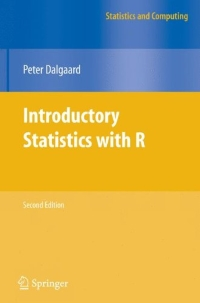
\includegraphics[width=2.78in]{figure/book1v2} 

}

\caption{https://goo.gl/zt7wc7 (Available for purchase online)}\label{fig:book1}
\end{figure}

\begin{figure}

{\centering 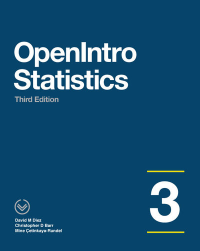
\includegraphics[width=2.78in]{figure/openintro.v2} 

}

\caption{https://www.openintro.org/stat/os4.php (Free!!!)}\label{fig:book2}
\end{figure}

\hypertarget{part1}{%
\chapter{Introduction}\label{part1}}

\hypertarget{r-and-rstudio}{%
\section{R and RStudio}\label{r-and-rstudio}}


\includegraphics{figure/r_and_rstudio.png}

\hypertarget{what-is-r}{%
\subsection{\texorpdfstring{What is \textbf{R}?}{What is R?}}\label{what-is-r}}

\textbf{R} \ldots{}

\begin{itemize}
\tightlist
\item
  is a free, open source program for statistical computing and data visualization.
\item
  is cross-platform (e.g., available on Windows, Mac OS, and Linux).
\item
  is maintained and reguarly updated by the Comprehensive R Archive Network (\href{https://cran.r-project.org/}{CRAN}.
\item
  is capable of running all types of statistical analyses.
\item
  has amazing visualization capabilities (high-quality, customizable figures).
\item
  enables reproducible research.
\item
  has many other capablities, such as web programming.
\item
  supports user-created packages (currently, more than 10,000)
\end{itemize}

\hypertarget{what-is-rstudio}{%
\subsection{What is RStudio?}\label{what-is-rstudio}}

\textbf{RStudio} \ldots{}

\begin{itemize}
\tightlist
\item
  is a free program available to control \textbf{R}
\item
  provides a more user-friendly interface for \textbf{R}.
\item
  includes a set of tools to help you be more productive with \textbf{R}, such as:

  \begin{itemize}
  \tightlist
  \item
    A syntax-highlighting editor for highlighting your \textbf{R} codes
  \item
    Functions for helping you type the \textbf{R} codes (auto-completion)
  \item
    A variety of tools for creating and saving various plots (e.g., histograms, scatterplot)
  \item
    A workspace management tool for importing or exporting data
  \end{itemize}
\end{itemize}

\hypertarget{download-and-install}{%
\subsection{Download and Install}\label{download-and-install}}

To benefit from \textbf{RStudio}, both \textbf{R} and \textbf{RStudio} should be installed in your computer. \textbf{R} and \textbf{RStudio} are freely available from the following websites:

To download and install \textbf{R}:

\begin{enumerate}
\def\labelenumi{\arabic{enumi}.}
\tightlist
\item
  Go to \href{https://cran.r-project.org/}{\textbf{https://cran.r-project.org/}}
\item
  Click ``Download R for Mac/Windows''"
\item
  Download the appropriate file:
  • Windows users click Base, and download the installer for the latest R version
  • Mac users select the file R-3.X.X.pkg that aligns with your OS version
\item
  Follow the instructions of the installer.
\end{enumerate}

To download and install \textbf{RStudio}:

\begin{enumerate}
\def\labelenumi{\arabic{enumi}.}
\tightlist
\item
  Go to \href{https://www.rstudio.com/products/rstudio/download/}{\textbf{https://www.rstudio.com/products/rstudio/download/}}
\item
  Click ``Download'' under \emph{RStudio Desktop - Open Source License}
\item
  Select the install file for your OS
\item
  Follow the instructions of the installer.
\end{enumerate}

\hypertarget{preview-of-rstudio}{%
\subsection{Preview of RStudio}\label{preview-of-rstudio}}

After you open RStudio, you should see the following screen:

\begin{figure}
\centering
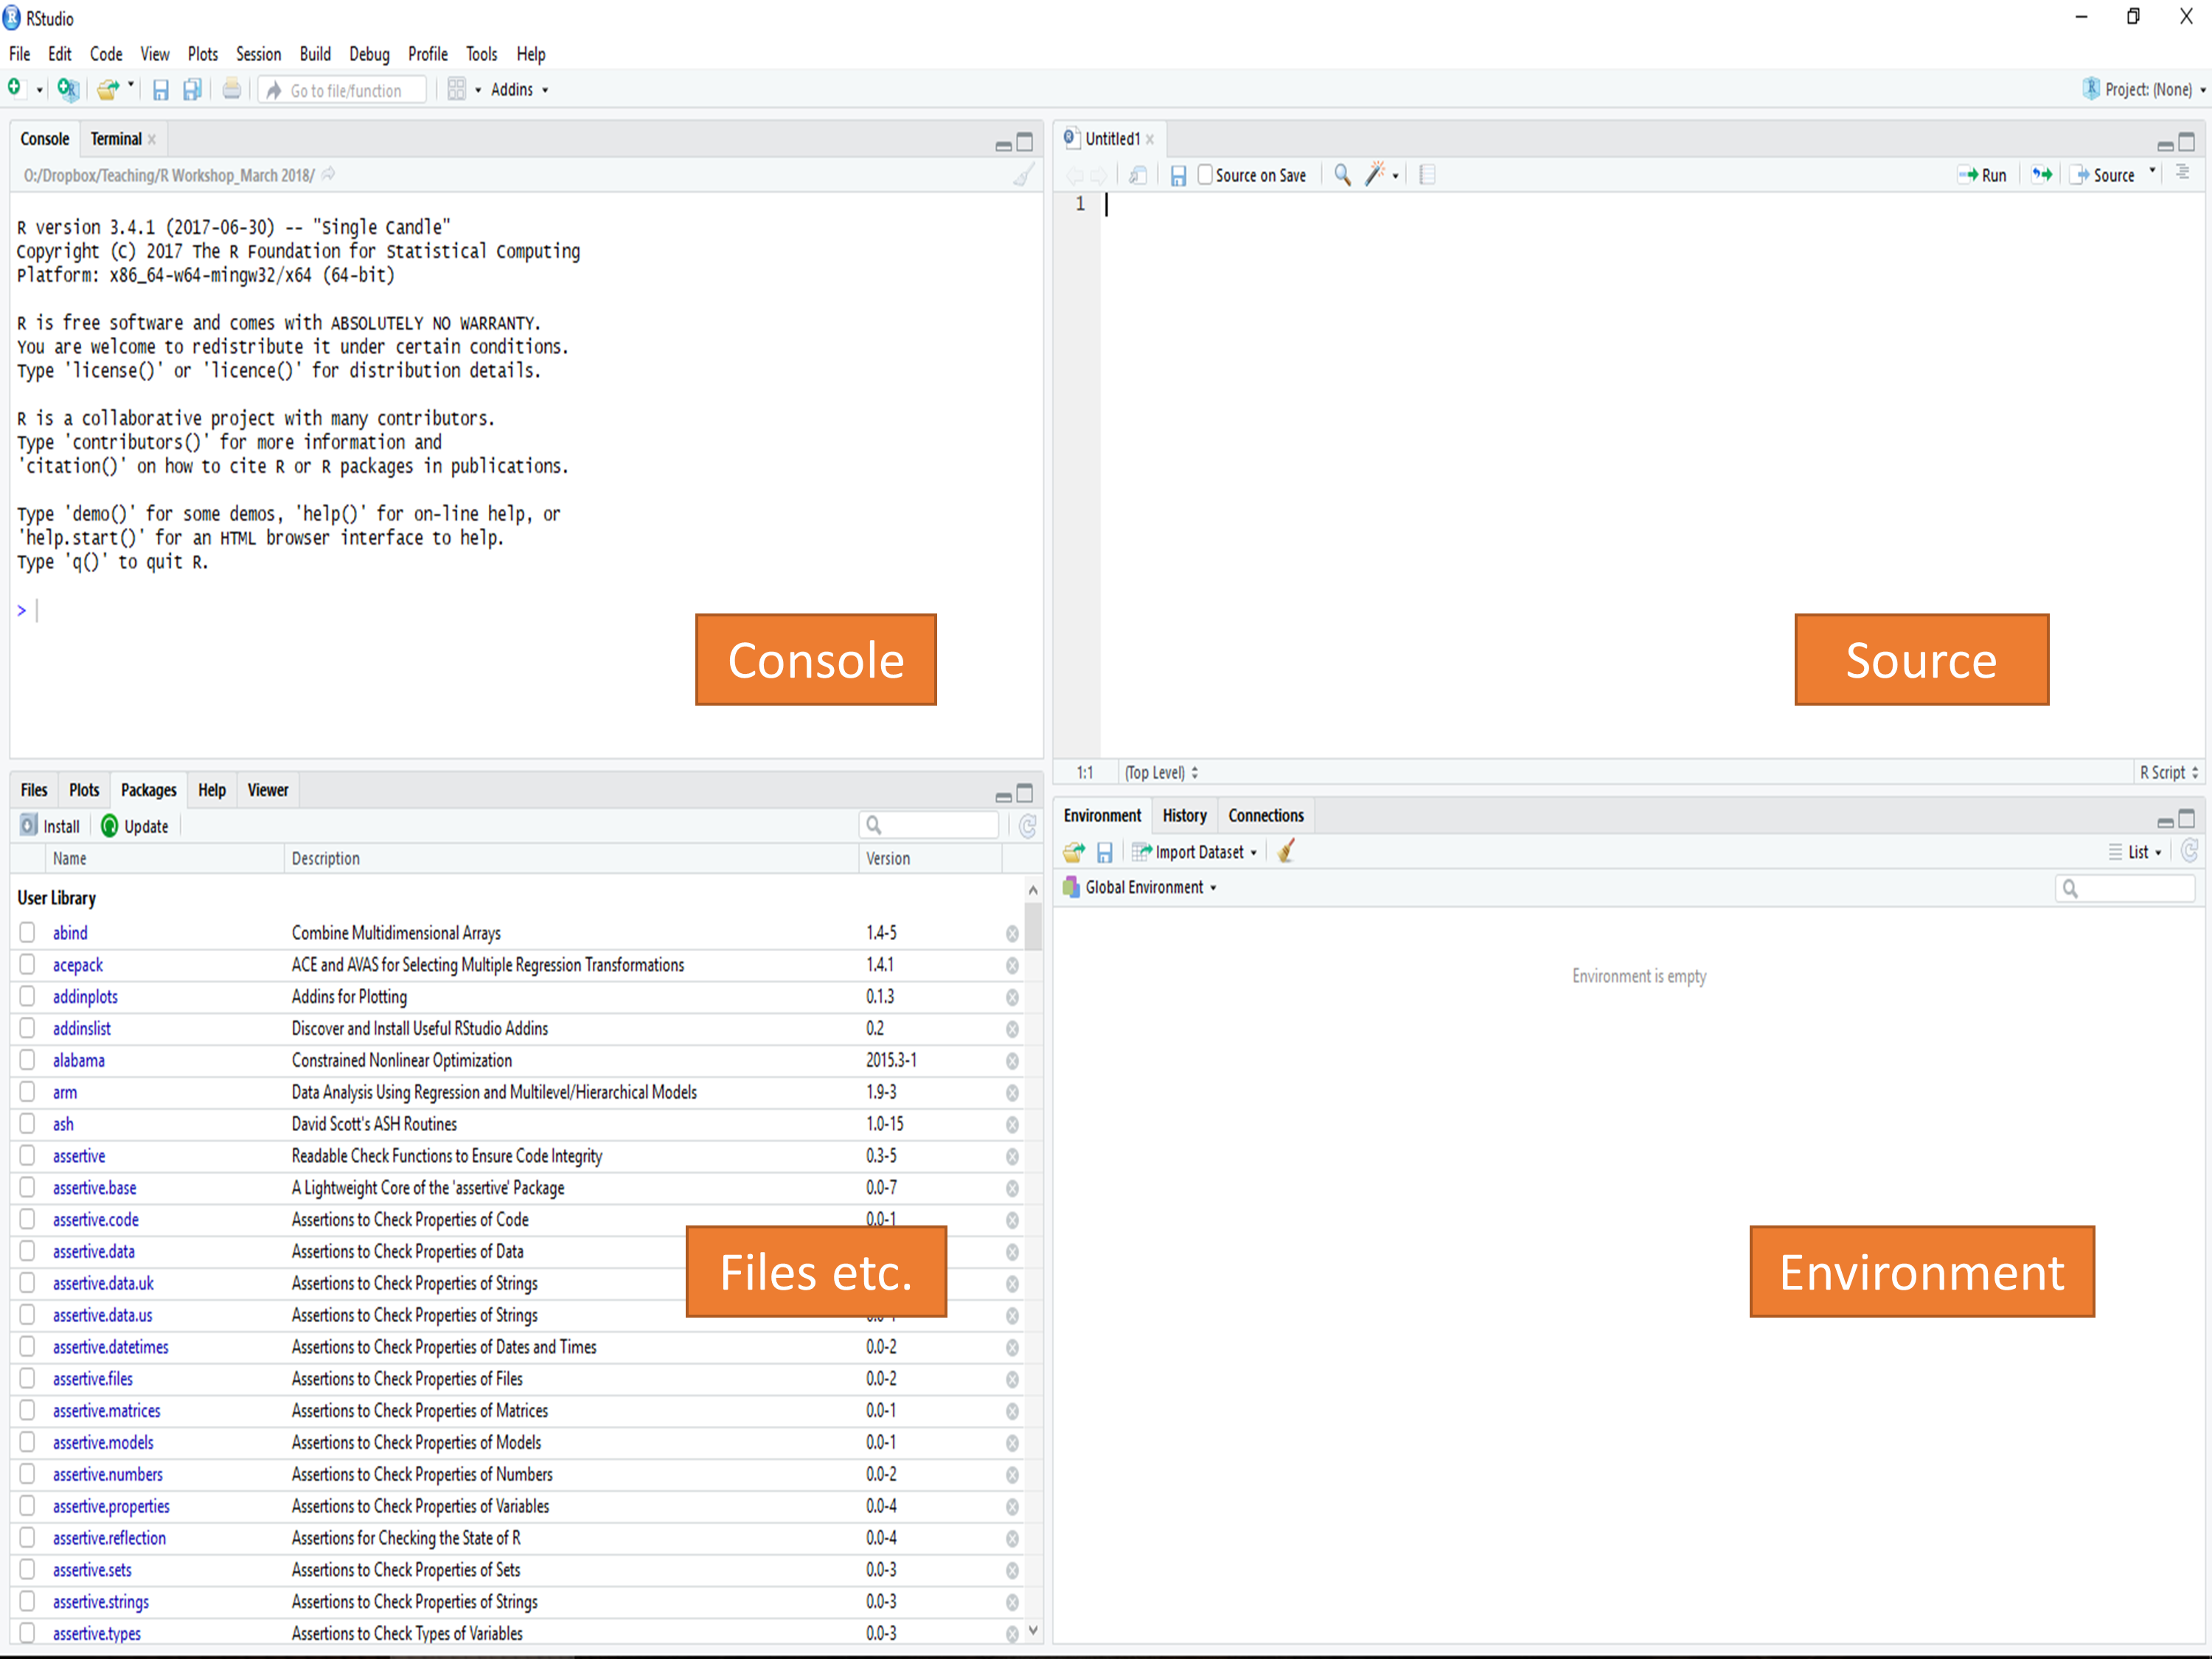
\includegraphics{figure/img1.png}
\caption{Opening screen of RStudio}
\end{figure}

I personally prefer console on the top-left, source on the top-right, files on the bottom-left, and environment on the bottom-right. The pane layout can be updated using \emph{Global Options} under \emph{Tools}.

\begin{figure}
\centering
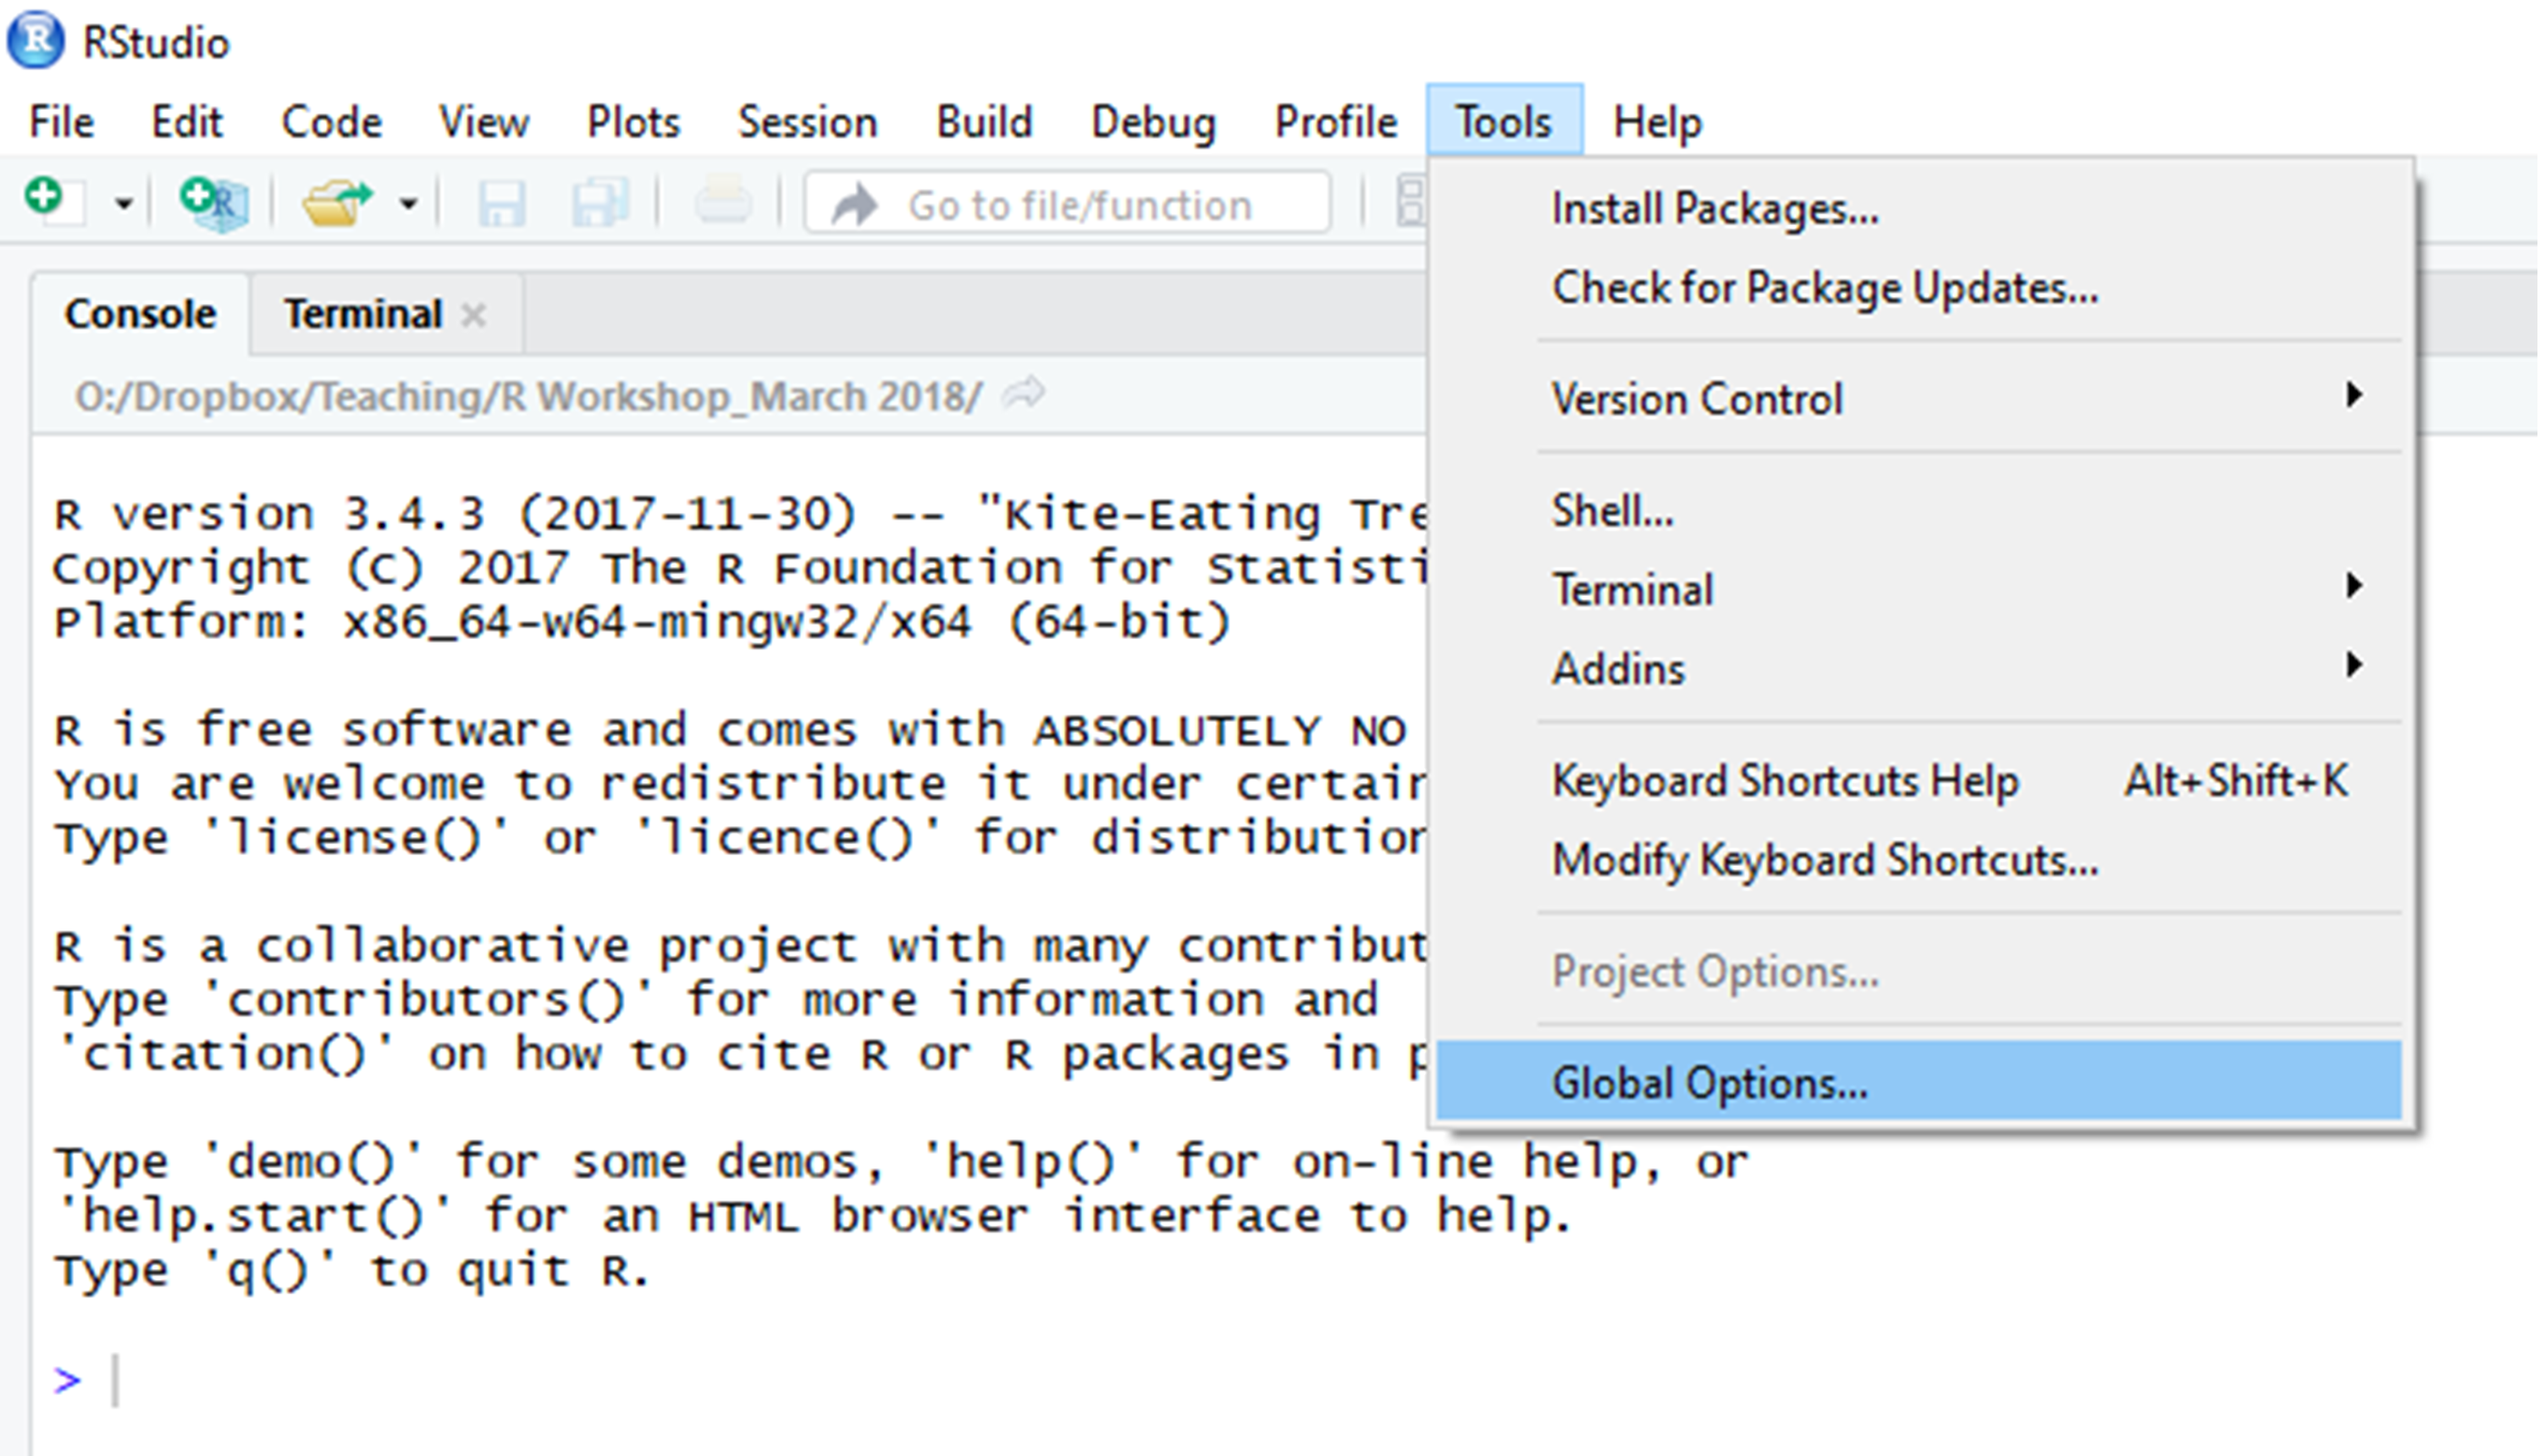
\includegraphics{figure/img2.png}
\caption{\textbf{Step 1:} Click Tools and then select Global Options}
\end{figure}

\begin{figure}
\centering
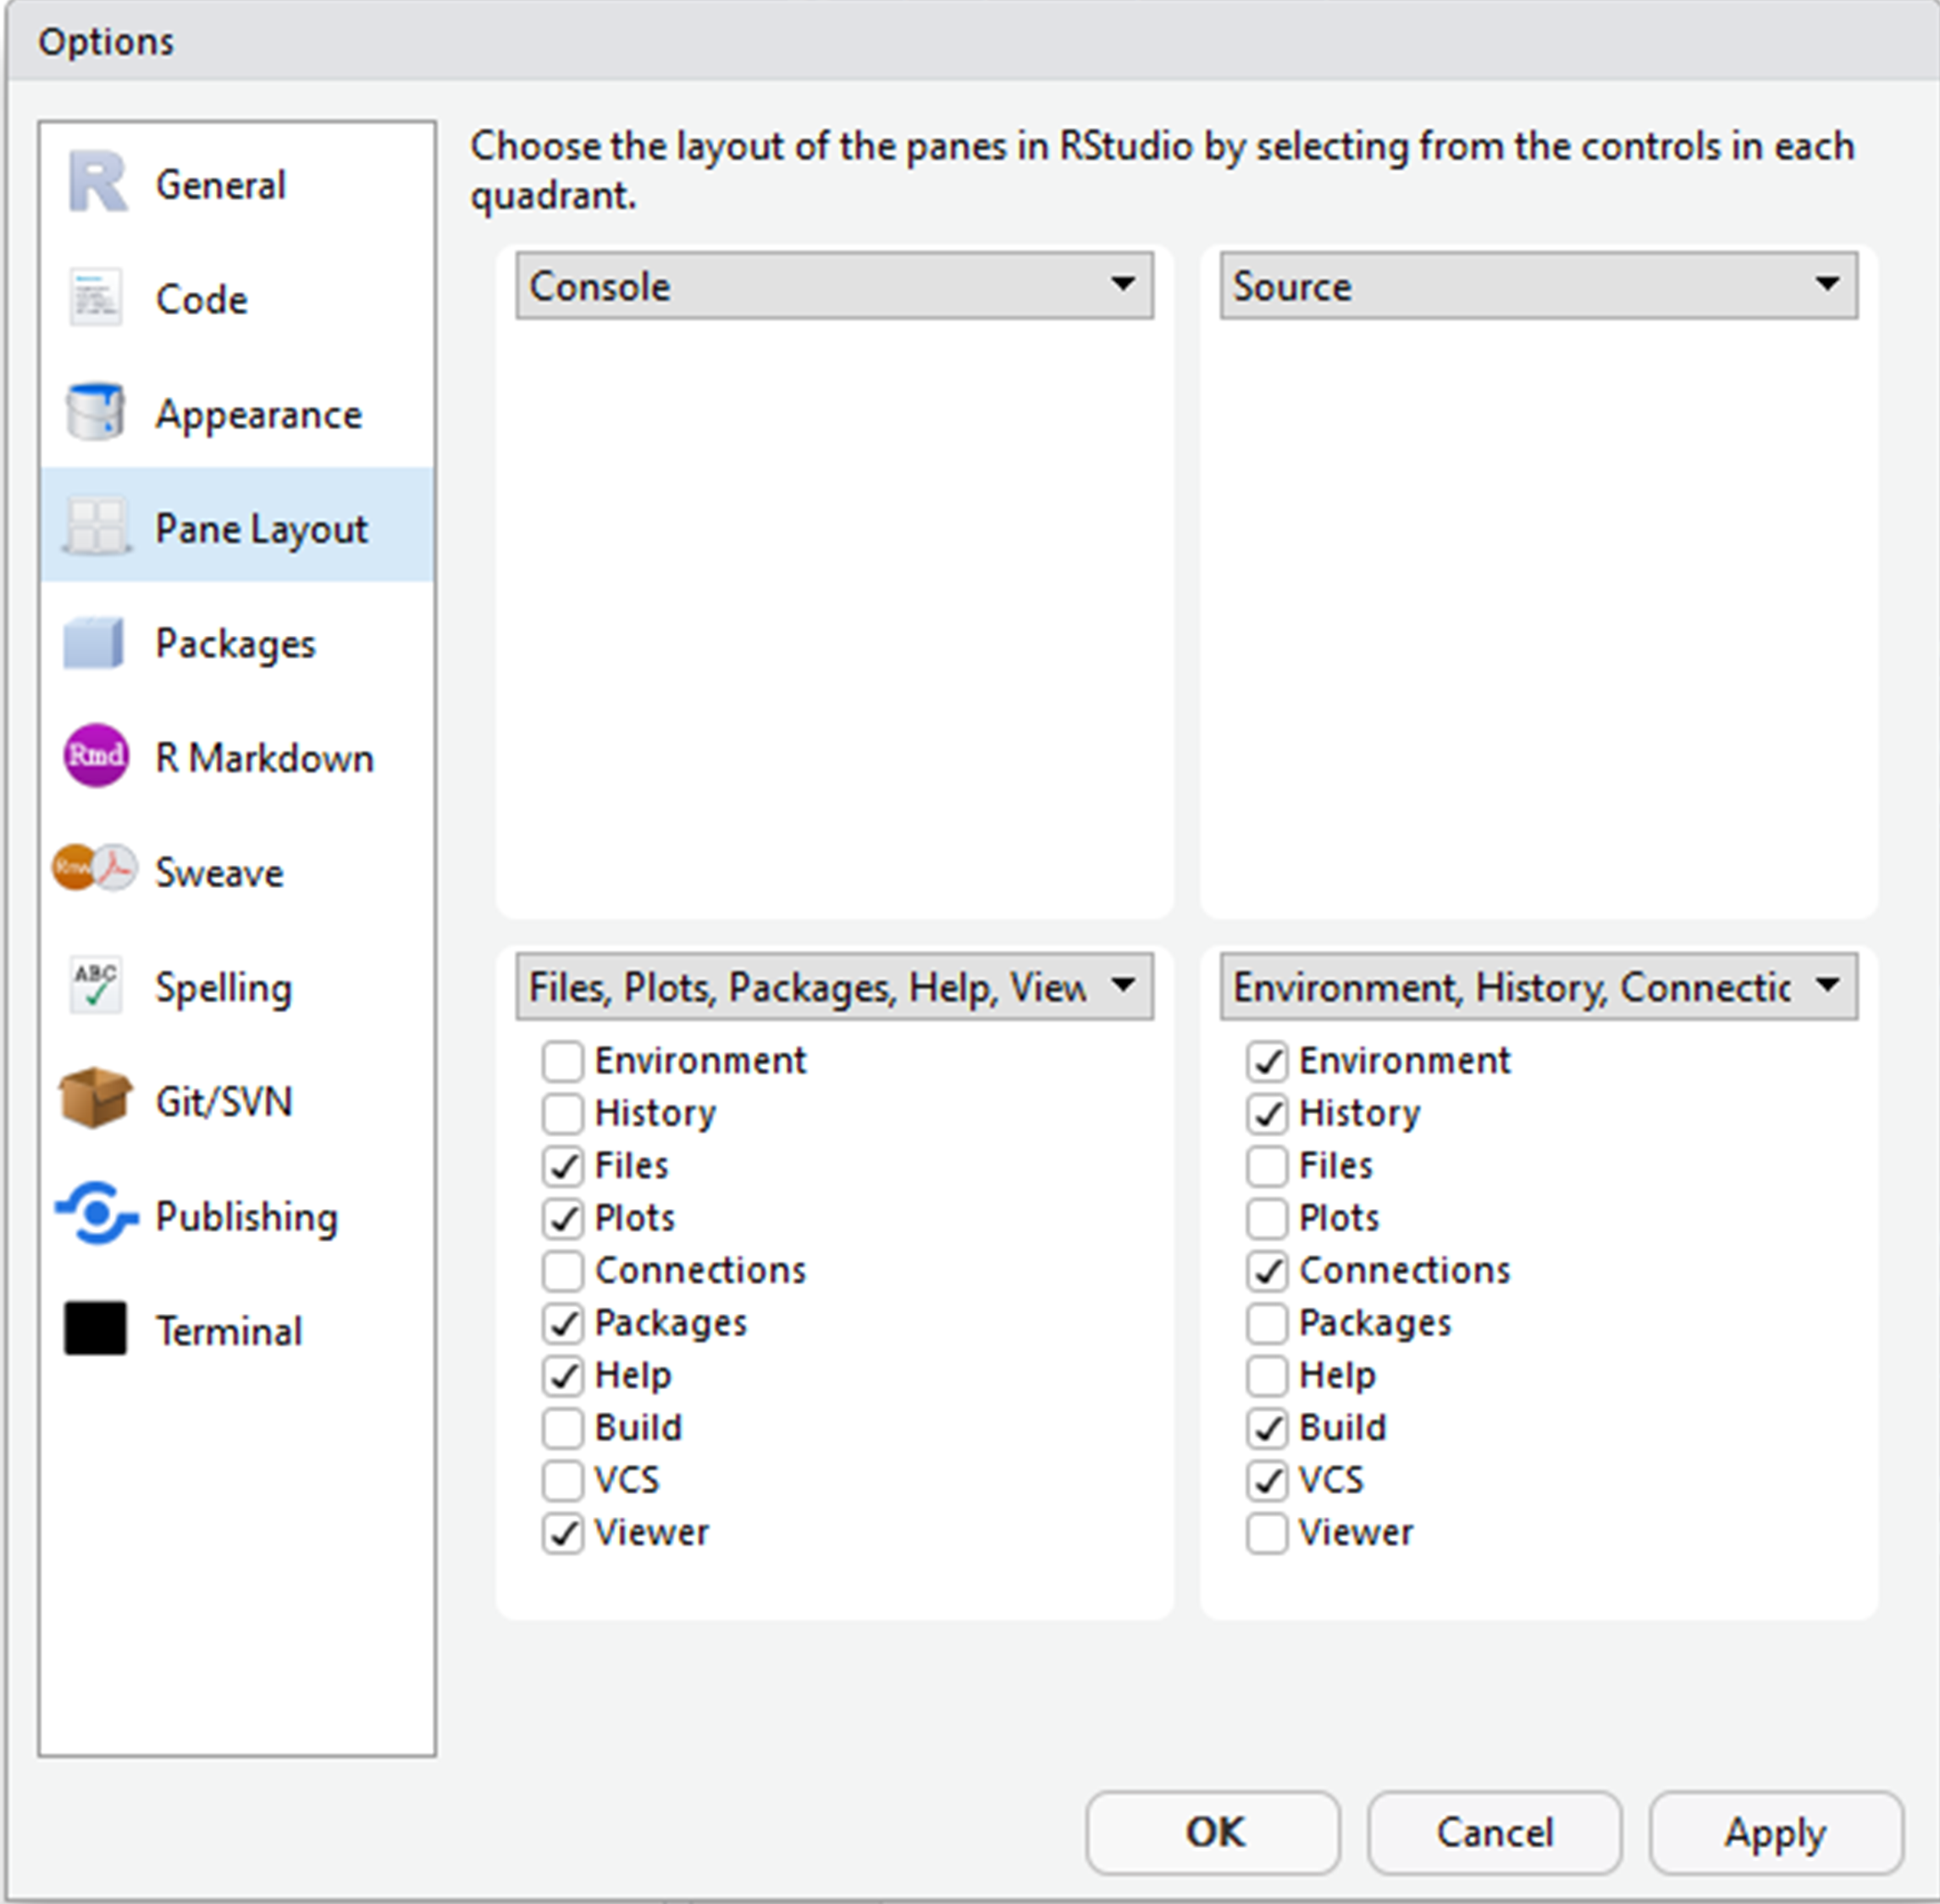
\includegraphics{figure/img3.png}
\caption{\textbf{Step 2:} Select console, source, environment, or files for each pane}
\end{figure}

We can also change the appearance (e.g., code highlighting, font type, font size, etc.):

\begin{figure}
\centering
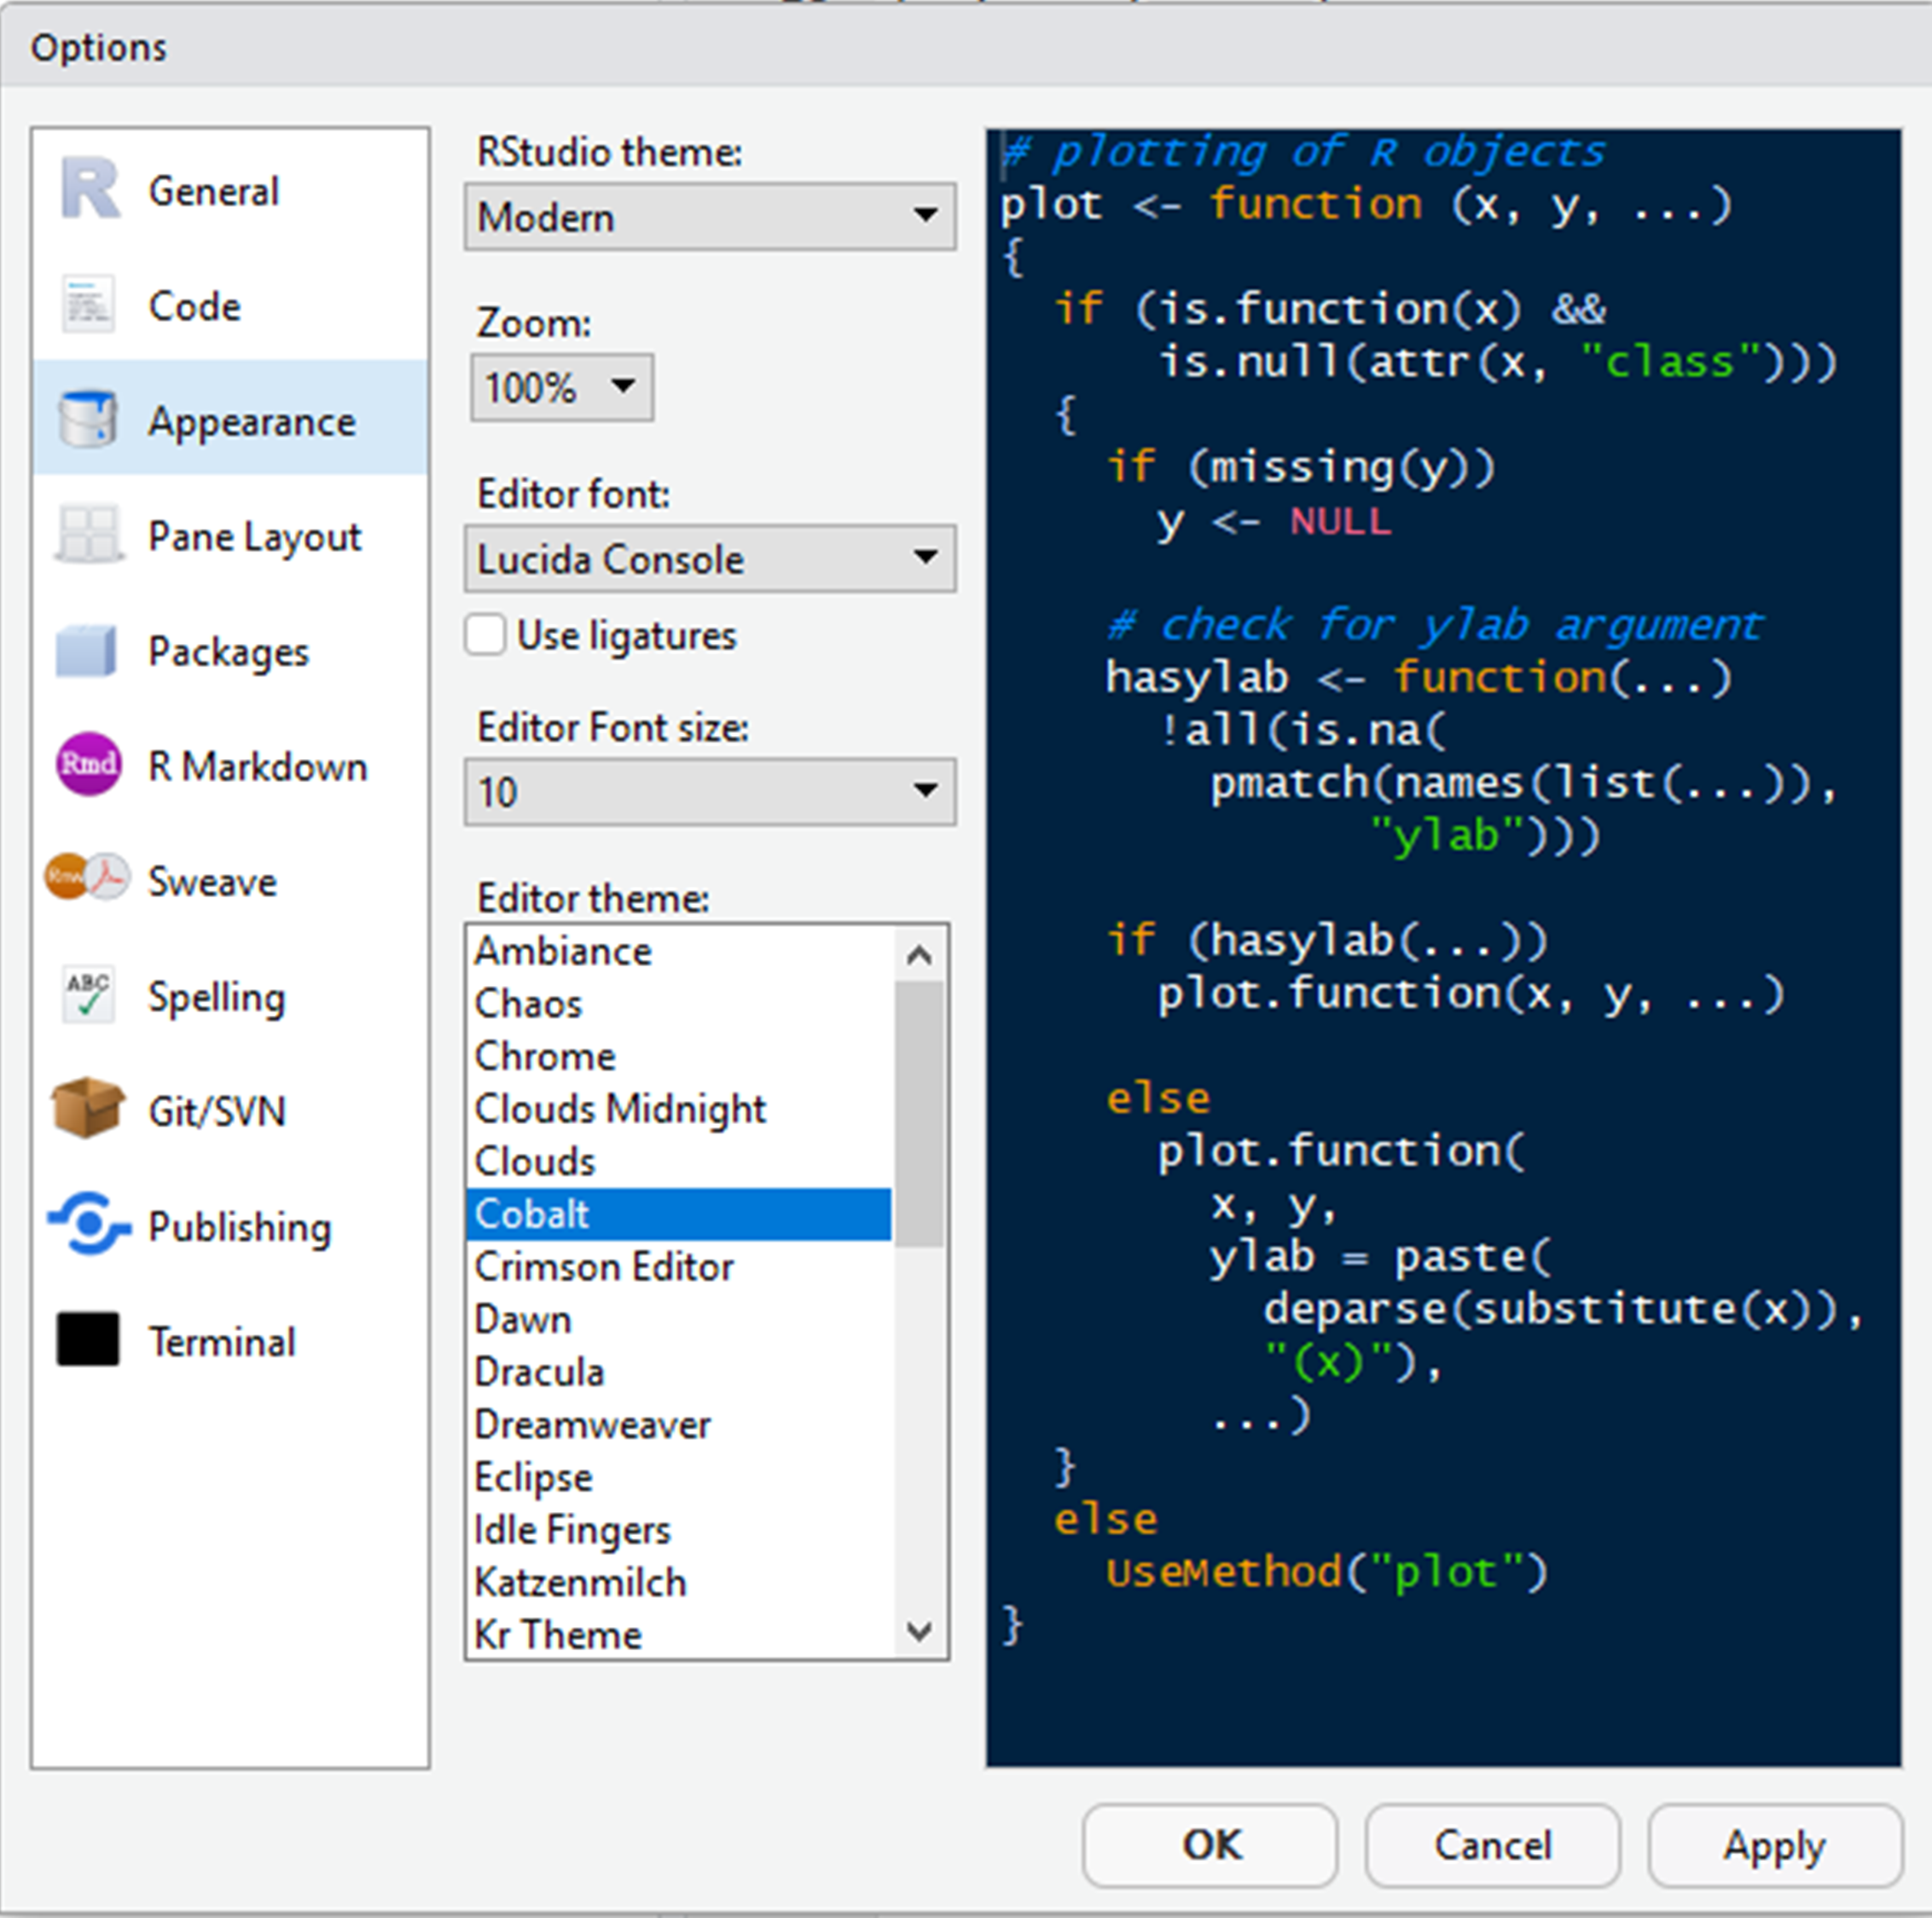
\includegraphics{figure/img4.png}
\caption{\textbf{Step 2:} Change the Appearance Settings, as you wish}
\end{figure}

\textbf{Note:} To get yourself more familiar with \textbf{RStudio}, I recommend you to check out the \textbf{RStudio} \href{https://github.com/okanbulut/rbook/blob/master/cheatsheets/rstudio-ide.pdf}{\textbf{cheatsheet}} and Oscar Torres-Reyna's nice \href{https://github.com/okanbulut/rbook/blob/master/cheatsheets/rstudio_tutorial.pdf}{\textbf{tutorial}} (\emph{Note:} You can click on these links to open and download the documents or see \url{https://github.com/okanbulut/rbook/tree/master/cheatsheets}).

\hypertarget{creating-a-new-script}{%
\subsection{Creating a New Script}\label{creating-a-new-script}}

In \textbf{R}, we can type our commands in the console; but once we close \textbf{R}, everything we have typed will be gone. Therefore, we should create an empty script, write the codes in the script, and save it for future use. We can replicate the exact same analysis and results by running the script again later on. The \textbf{R} script file has the .R extension, but it is essentially a text file. Thus, any text editor (e.g., Microsoft Word, Notepad, TextPad) can be used to open a script file for editing outside of the \textbf{R} environment.

We can create a new script file in \textbf{R} as follows:

\begin{figure}
\centering
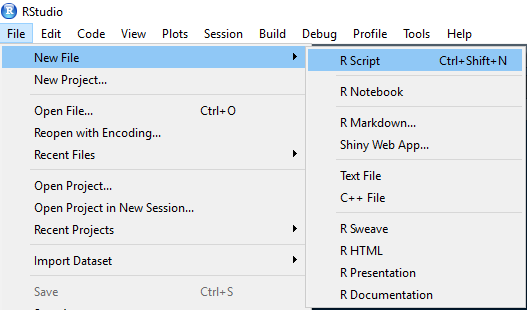
\includegraphics{figure/img5.png}
\caption{Creating a new script in \textbf{R} (using \textbf{RStudio})}
\end{figure}

When we type some codes in the script, we can select the lines we want to run and then hit the run button. Alternatively, we can bring the cursor at the beginning of the line and hit the run button which runs one line at a time and moves to the next line.

\begin{figure}
\centering
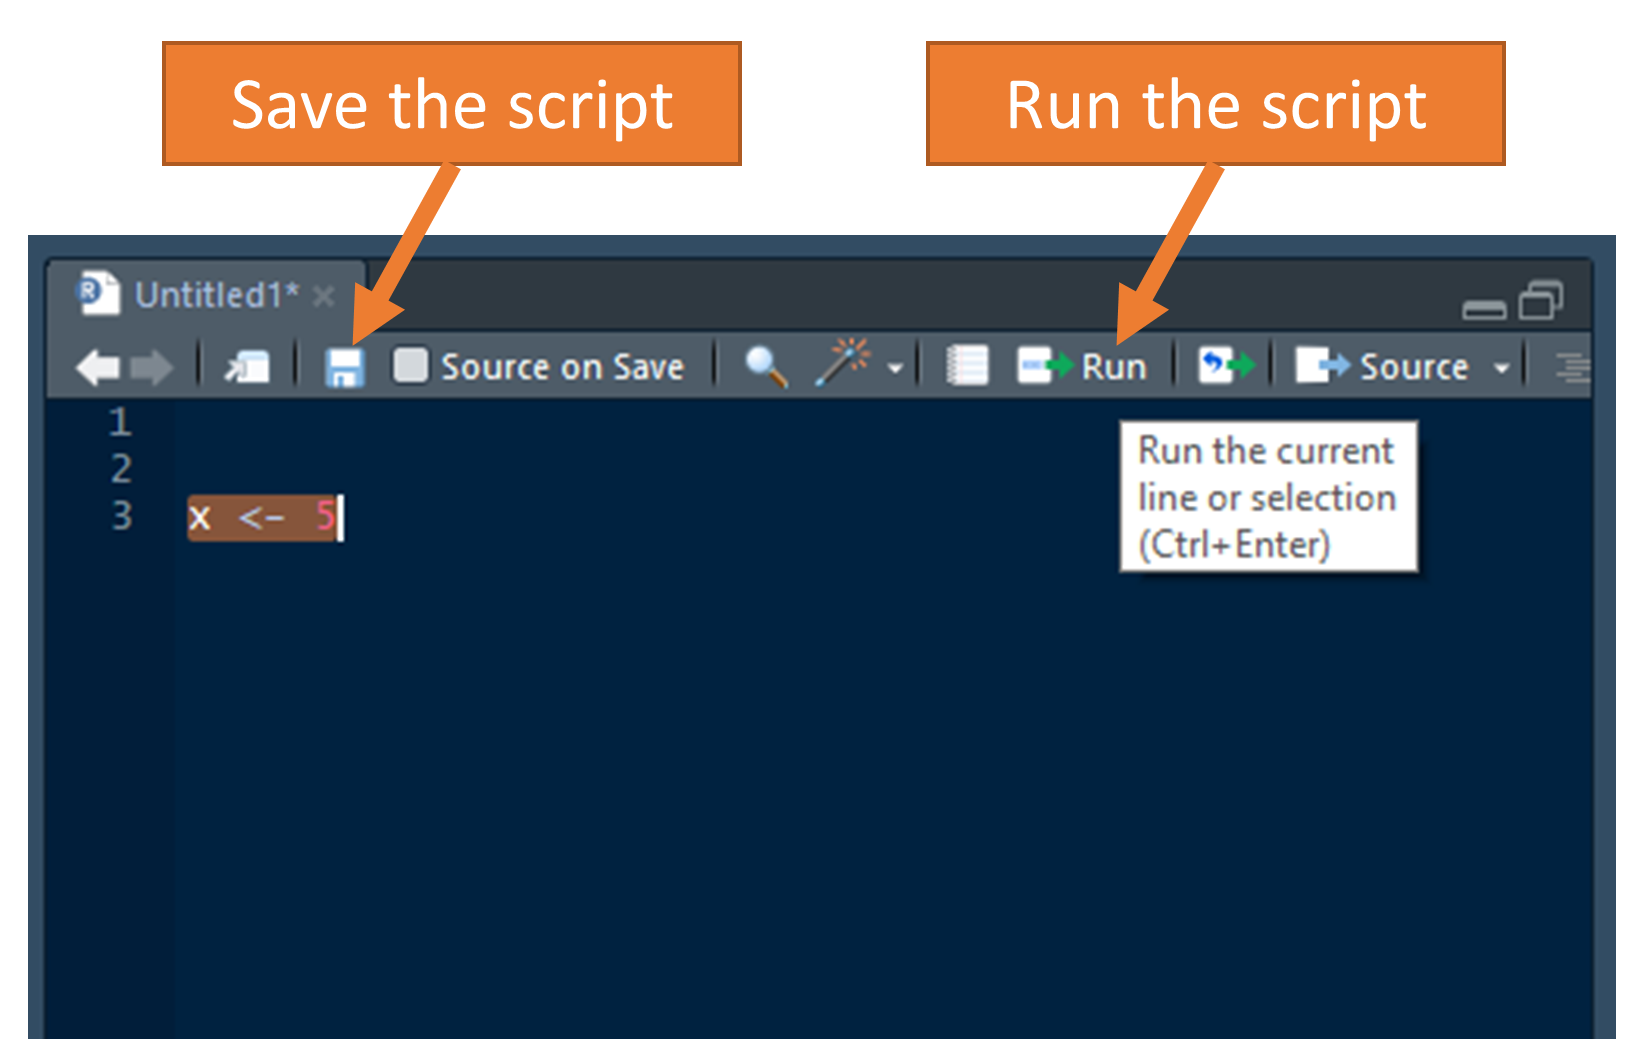
\includegraphics{figure/img7.png}
\caption{Running \textbf{R} codes from a script file}
\end{figure}

\hypertarget{working-directory}{%
\subsection{Working Directory}\label{working-directory}}

An important feature of \textbf{R} is ``working directory'', which refers to a location or a folder in your computer where you keep your \textbf{R} script, your data files, etc. Once we define a working directory in \textbf{R}, any data file or script within that directory can be easily imported into \textbf{R} without specifying where the file is located. By default, \textbf{R} chooses a particular location in your computer (typically Desktop or Documents) as your working director. To see our current working director, we need to run a \texttt{getwd()} command in the \textbf{R} console:

\begin{Shaded}
\begin{Highlighting}[]
\KeywordTok{getwd}\NormalTok{()}
\end{Highlighting}
\end{Shaded}

This will return a path like this:

\begin{Shaded}
\begin{Highlighting}[]
\CommentTok{## [1] "C:/Users/bulut/Desktop"}
\end{Highlighting}
\end{Shaded}

Once we decide to change the current working direcory into a different location, we can do it in two ways:

\textbf{Method 1:} Using the ``Session'' options menu in \textbf{RStudio}

We can select Session \textgreater{} Set Working Directory \textgreater{} Choose Directory to find a folder or location that we want to set as our current working directory.

\begin{figure}
\centering
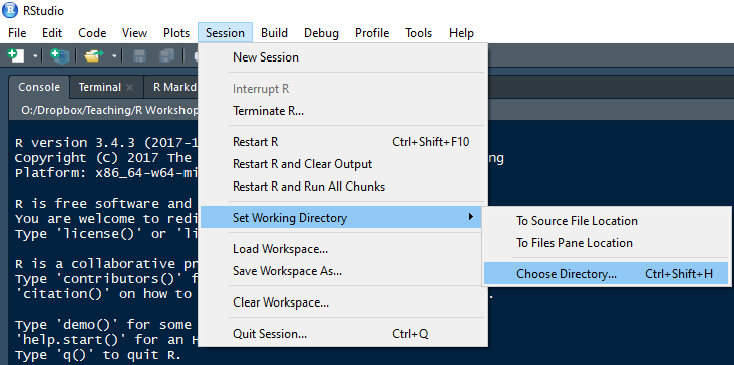
\includegraphics{figure/img6.png}
\caption{\textbf{Method 1:} Setting the working directory in \textbf{R}}
\end{figure}

\textbf{Method 2:} Using the \texttt{setwd} command in the console

Tpying the following code in the console will set the ``R workshop'' folder on my desktop as the working directory. If the folder path is correct, \textbf{R} changes the working directory without giving any error messages in the console.

\begin{Shaded}
\begin{Highlighting}[]
\KeywordTok{setwd}\NormalTok{(}\StringTok{"C:/Users/bulut/Desktop/R workshop"}\NormalTok{)}
\end{Highlighting}
\end{Shaded}

To ensure that the working directory is properly set, we can use the \texttt{getwd()} command again:

\begin{Shaded}
\begin{Highlighting}[]
\KeywordTok{getwd}\NormalTok{()}
\CommentTok{## [1] "C:/Users/bulut/Desktop/R workshop"}
\end{Highlighting}
\end{Shaded}

\textbf{IMPORTANT:} \textbf{R} does not accept any backslashes in the file path. Instead of a backslash, we need to use a frontslash. This is particulary important for Windows computers since the file paths involve backslashes (Mac OS X doesn't have this problem).

\hypertarget{downloading-and-installing-r-packages}{%
\subsection{\texorpdfstring{Downloading and Installing \textbf{R} Packages}{Downloading and Installing R Packages}}\label{downloading-and-installing-r-packages}}

The base \textbf{R} program comes with many built-in functions to compute a variety of statistics and to create graphics (e.g., histograms, scatterplots, etc.). However, what makes \textbf{R} more powerful than other software programs is that \textbf{R} users can write their own functions, put them in a package, and share it with other \textbf{R} users via the \href{https://cran.r-project.org/web/packages/index.html}{CRAN} website.

For example, \texttt{ggplot2} \citep{R-ggplot2} is a well-known \textbf{R} package, created by Hadley Wickham and Winston Chang. This package allows \textbf{R} users to create elegant data visualizations. To download and install the \texttt{ggplot2} package, we need to use the \texttt{install.packages} command. Note that your computer has to be connected to the internet to be able to connect to the CRAN website and download the package.

\begin{Shaded}
\begin{Highlighting}[]
\KeywordTok{install.packages}\NormalTok{(}\StringTok{"ggplot2"}\NormalTok{)}
\end{Highlighting}
\end{Shaded}

Once a package is downloaded and installed, it is permanently in your \textbf{R} folder. That is, there is no need to re-install it, unless you remove the package or install a new version of R. These downloaded packages are not directly accessible until we activate them in your \textbf{R} session. Whenever we need to access a package in \textbf{R}, we need to use the \texttt{library} command to activate it. For example, to access the \texttt{ggplot2} package, we would use:

\begin{Shaded}
\begin{Highlighting}[]
\KeywordTok{library}\NormalTok{(}\StringTok{"ggplot2"}\NormalTok{)}
\end{Highlighting}
\end{Shaded}

To get help on installed packages (e.g., what's inside this package):

\begin{Shaded}
\begin{Highlighting}[]
\CommentTok{# To get details regarding contents of a package}
\KeywordTok{help}\NormalTok{(}\DataTypeTok{package =} \StringTok{"ggplot2"}\NormalTok{)}

\CommentTok{# To list vignettes available for a specific package}
\KeywordTok{vignette}\NormalTok{(}\DataTypeTok{package =} \StringTok{"ggplot2"}\NormalTok{)}

\CommentTok{# To view specific vignette}
\KeywordTok{vignette}\NormalTok{(}\StringTok{"ggplot2-specs"}\NormalTok{)}
\end{Highlighting}
\end{Shaded}

\hypertarget{your-turn}{%
\subsection{Your turn}\label{your-turn}}

\begin{enumerate}
\def\labelenumi{\arabic{enumi}.}
\tightlist
\item
  Open \textbf{RStudio} and find the Global Settings option and change the pane layout as you like. I recommend putting the console on the top-left corner.
\item
  Set the folder that you have the training materials (it's called \emph{rtraining}) as your working directory using either the \texttt{setwd} command or the Session options menu in **RStudio*.
\item
  Create a new script and click the save button -- which will ask you to save it. Name it as ``mysyntax.R'' and save it in the same folder (rtraining).\\
\item
  Install and activate the \texttt{lattice} package using the \texttt{install.packages} and \texttt{library} commands. The \texttt{lattice} package \citep{R-lattice} is another well-known package for data visualization in \textbf{R}. You should type the following in your script file, choose all the lines, and hit the run button.
\end{enumerate}

\begin{Shaded}
\begin{Highlighting}[]
\KeywordTok{install.packages}\NormalTok{(}\StringTok{"lattice"}\NormalTok{)}
\KeywordTok{library}\NormalTok{(}\StringTok{"lattice"}\NormalTok{)}
\end{Highlighting}
\end{Shaded}

\hypertarget{basics-of-the-r-language}{%
\section{Basics of the R Language}\label{basics-of-the-r-language}}

\hypertarget{r-as-a-calculator}{%
\subsection{R as a Calculator}\label{r-as-a-calculator}}

\textbf{R} can be used like a calculator to do addition, subtraction, multiplication, and division. For example, if you type the following in the console, you should see the results in the same window.

\begin{Shaded}
\begin{Highlighting}[]
\DecValTok{20} \OperatorTok{+}\StringTok{ }\NormalTok{(}\DecValTok{30} \OperatorTok{*}\StringTok{ }\DecValTok{3}\NormalTok{)}
\end{Highlighting}
\end{Shaded}

\begin{verbatim}
[1] 110
\end{verbatim}

\begin{Shaded}
\begin{Highlighting}[]
\NormalTok{(}\DecValTok{144}\OperatorTok{/}\DecValTok{12}\NormalTok{) }\OperatorTok{-}\StringTok{ }\NormalTok{(}\DecValTok{20}\OperatorTok{/}\DecValTok{5}\NormalTok{)}
\end{Highlighting}
\end{Shaded}

\begin{verbatim}
[1] 8
\end{verbatim}

More complex calculations are also possible in \textbf{R}.

\begin{Shaded}
\begin{Highlighting}[]
\DecValTok{10}\OperatorTok{^}\DecValTok{2}
\end{Highlighting}
\end{Shaded}

\begin{verbatim}
[1] 100
\end{verbatim}

\begin{Shaded}
\begin{Highlighting}[]
\KeywordTok{sqrt}\NormalTok{(}\DecValTok{81}\NormalTok{)}
\end{Highlighting}
\end{Shaded}

\begin{verbatim}
[1] 9
\end{verbatim}

\begin{Shaded}
\begin{Highlighting}[]
\KeywordTok{log}\NormalTok{(}\DecValTok{5}\NormalTok{)}
\end{Highlighting}
\end{Shaded}

\begin{verbatim}
[1] 1.609
\end{verbatim}

\begin{Shaded}
\begin{Highlighting}[]
\KeywordTok{exp}\NormalTok{(}\FloatTok{1.5}\NormalTok{)}
\end{Highlighting}
\end{Shaded}

\begin{verbatim}
[1] 4.482
\end{verbatim}

\hypertarget{creating-new-variables}{%
\subsection{Creating New Variables}\label{creating-new-variables}}

To create a new variable in R, we use the assignment operator, \texttt{\textless{}-}. To create a variable \texttt{x} that equals 25, we need to type:

\begin{Shaded}
\begin{Highlighting}[]
\NormalTok{x <-}\StringTok{ }\DecValTok{25}
\end{Highlighting}
\end{Shaded}

If we want to print \texttt{x}, we just type \texttt{x} in the console and hit enter. \textbf{R} returns the value assigned to \texttt{x}.

\begin{Shaded}
\begin{Highlighting}[]
\NormalTok{x}
\end{Highlighting}
\end{Shaded}

\begin{verbatim}
[1] 25
\end{verbatim}

We can also create a variable that holds multiple values in it, using the \texttt{c} command (\texttt{c} standards for \emph{combine}).

\begin{Shaded}
\begin{Highlighting}[]
\NormalTok{weight <-}\StringTok{ }\KeywordTok{c}\NormalTok{(}\DecValTok{60}\NormalTok{, }\DecValTok{72}\NormalTok{, }\DecValTok{80}\NormalTok{, }\DecValTok{84}\NormalTok{, }\DecValTok{56}\NormalTok{)}
\NormalTok{weight}
\end{Highlighting}
\end{Shaded}

\begin{verbatim}
[1] 60 72 80 84 56
\end{verbatim}

\begin{Shaded}
\begin{Highlighting}[]
\NormalTok{height <-}\StringTok{ }\KeywordTok{c}\NormalTok{(}\FloatTok{1.7}\NormalTok{, }\FloatTok{1.75}\NormalTok{, }\FloatTok{1.8}\NormalTok{, }\FloatTok{1.9}\NormalTok{, }\FloatTok{1.6}\NormalTok{)}
\NormalTok{height}
\end{Highlighting}
\end{Shaded}

\begin{verbatim}
[1] 1.70 1.75 1.80 1.90 1.60
\end{verbatim}

Once we create a variable, we can do further calculations with it. Let's say we want to transform the \texttt{weight} variable (in kg) to a new variable called weight2 (in lbs).

\begin{Shaded}
\begin{Highlighting}[]
\NormalTok{weight2 <-}\StringTok{ }\NormalTok{weight }\OperatorTok{*}\StringTok{ }\FloatTok{2.20462}
\NormalTok{weight2}
\end{Highlighting}
\end{Shaded}

\begin{verbatim}
[1] 132.3 158.7 176.4 185.2 123.5
\end{verbatim}

Note that we named the variable as \texttt{weight2}. So, both \texttt{weight} and \texttt{weight2} exist in the active \textbf{R} session now. If we used the following, this would overwrite the existing \texttt{weight} variable.

\begin{Shaded}
\begin{Highlighting}[]
\NormalTok{weight <-}\StringTok{ }\NormalTok{weight }\OperatorTok{*}\StringTok{ }\FloatTok{2.20462}
\end{Highlighting}
\end{Shaded}

We can also define a new variable based on existing variables.

\begin{Shaded}
\begin{Highlighting}[]
\NormalTok{reading <-}\StringTok{ }\KeywordTok{c}\NormalTok{(}\DecValTok{80}\NormalTok{, }\DecValTok{75}\NormalTok{, }\DecValTok{50}\NormalTok{, }\DecValTok{44}\NormalTok{, }\DecValTok{65}\NormalTok{)}
\NormalTok{math <-}\StringTok{ }\KeywordTok{c}\NormalTok{(}\DecValTok{90}\NormalTok{, }\DecValTok{65}\NormalTok{, }\DecValTok{60}\NormalTok{, }\DecValTok{38}\NormalTok{, }\DecValTok{70}\NormalTok{)}
\NormalTok{total <-}\StringTok{ }\NormalTok{reading }\OperatorTok{+}\StringTok{ }\NormalTok{math}
\NormalTok{total}
\end{Highlighting}
\end{Shaded}

\begin{verbatim}
[1] 170 140 110  82 135
\end{verbatim}

Sometimes we need a variable that holds character strings rather than numerical values. If a value is not numerical, we need to use double quotation marks. In the example below, we create a new variable called \texttt{cities} that has four city names in it. Each city name is written with double quotation marks.

\begin{Shaded}
\begin{Highlighting}[]
\NormalTok{cities <-}\StringTok{ }\KeywordTok{c}\NormalTok{(}\StringTok{"Edmonton"}\NormalTok{, }\StringTok{"Calgary"}\NormalTok{, }\StringTok{"Red Deer"}\NormalTok{, }\StringTok{"Spruce Grove"}\NormalTok{)}
\NormalTok{cities}
\end{Highlighting}
\end{Shaded}

\begin{verbatim}
[1] "Edmonton"     "Calgary"      "Red Deer"     "Spruce Grove"
\end{verbatim}

We can also treat numerical values as character strings. For example, assume that we have a \texttt{gender} variable where 1=Male and 2=Female. We want R to know that these values are not actual numbers; instead, they are just numerical labels for gender groups.

\begin{Shaded}
\begin{Highlighting}[]
\NormalTok{gender <-}\StringTok{ }\KeywordTok{c}\NormalTok{(}\StringTok{"1"}\NormalTok{, }\StringTok{"2"}\NormalTok{, }\StringTok{"2"}\NormalTok{, }\StringTok{"1"}\NormalTok{, }\StringTok{"2"}\NormalTok{)}
\NormalTok{gender}
\end{Highlighting}
\end{Shaded}

\begin{verbatim}
[1] "1" "2" "2" "1" "2"
\end{verbatim}

\hypertarget{important-rules-for-the-r-language}{%
\subsection{\texorpdfstring{Important Rules for the \textbf{R} Language}{Important Rules for the R Language}}\label{important-rules-for-the-r-language}}

Here is a list of important rules for using the \textbf{R} language more effectively:

\begin{enumerate}
\def\labelenumi{\arabic{enumi}.}
\tightlist
\item
  \textbf{Case-sensitivity:} \textbf{R} codes written in lowercase would NOT refer to the same codes written in uppercase.
\end{enumerate}

\begin{Shaded}
\begin{Highlighting}[]
\NormalTok{cities <-}\StringTok{ }\KeywordTok{c}\NormalTok{(}\StringTok{"Edmonton"}\NormalTok{, }\StringTok{"Calgary"}\NormalTok{, }\StringTok{"Red Deer"}\NormalTok{, }\StringTok{"Spruce Grove"}\NormalTok{)}
\NormalTok{Cities}
\NormalTok{CITIES}

\NormalTok{Error}\OperatorTok{:}\StringTok{ }\NormalTok{object }\StringTok{'Cities'}\NormalTok{ not found}
\NormalTok{Error}\OperatorTok{:}\StringTok{ }\NormalTok{object }\StringTok{'CITIES'}\NormalTok{ not found}
\end{Highlighting}
\end{Shaded}

\begin{enumerate}
\def\labelenumi{\arabic{enumi}.}
\setcounter{enumi}{1}
\tightlist
\item
  \textbf{Variable names:} A variable name \textbf{cannot} begin with a number or include a space.
\end{enumerate}

\begin{Shaded}
\begin{Highlighting}[]
\NormalTok{4cities <-}\StringTok{ }\KeywordTok{c}\NormalTok{(}\StringTok{"Edmonton"}\NormalTok{, }\StringTok{"Calgary"}\NormalTok{, }\StringTok{"Red Deer"}\NormalTok{, }\StringTok{"Spruce Grove"}\NormalTok{)}
\NormalTok{my cities <-}\StringTok{ }\KeywordTok{c}\NormalTok{(}\StringTok{"Edmonton"}\NormalTok{, }\StringTok{"Calgary"}\NormalTok{, }\StringTok{"Red Deer"}\NormalTok{, }\StringTok{"Spruce Grove"}\NormalTok{)}

\NormalTok{Error}\OperatorTok{:}\StringTok{ }\NormalTok{unexpected symbol }\ControlFlowTok{in} \StringTok{"4cities"}
\NormalTok{Error}\OperatorTok{:}\StringTok{ }\NormalTok{unexpected symbol }\ControlFlowTok{in} \StringTok{"my cities"}
\end{Highlighting}
\end{Shaded}

\begin{enumerate}
\def\labelenumi{\arabic{enumi}.}
\setcounter{enumi}{2}
\item
  \textbf{Naming conventions:} Not to create messy codes that are difficult to read and understand, I recommend using consistent and clear naming conventions. I personally prefer all lowercase with underscore (e.g., \texttt{my\_variable}). The other naming conventions are:

  \begin{itemize}
  \tightlist
  \item
    All lowercase: e.g.~\texttt{mycities}
  \item
    Period.separated: e.g.~\texttt{my.cities}
  \item
    Underscore\_separated: e.g.~\texttt{my\_cities}
  \item
    Numbers at the end: e.g.~\texttt{mycities2018}
  \item
    Combination of some of these rules: \texttt{my.cities.2018}
  \end{itemize}
\item
  \textbf{Commenting:} The hashtag symbol (\#) is used for commenting in R. Any words, codes, etc. coming after a hashtag are just ignored. I strongly recommend using comments throughout your codes. These annotations would remind you what you did and why you did it that way. You can easily comment out a line without having to remove it from your codes.
\end{enumerate}

\begin{Shaded}
\begin{Highlighting}[]
\CommentTok{# Here I define four cities in Alberta}
\NormalTok{cities <-}\StringTok{ }\KeywordTok{c}\NormalTok{(}\StringTok{"Edmonton"}\NormalTok{, }\StringTok{"Calgary"}\NormalTok{, }\StringTok{"Red Deer"}\NormalTok{, }\StringTok{"Spruce Grove"}\NormalTok{)}
\end{Highlighting}
\end{Shaded}

\hypertarget{a-few-shortcuts}{%
\subsection{A Few Shortcuts}\label{a-few-shortcuts}}

\begin{itemize}
\item
  To list all objects (e.g., variables, results, etc.): \texttt{ls()}
\item
  To list and describe all objects: \texttt{ls.str()}
\item
  To remove a defined variable or data from the \textbf{R} environment: \texttt{rm()}

  \begin{itemize}
  \tightlist
  \item
    For example, we can remove the \texttt{age} variable as \texttt{rm(age)}
  \end{itemize}
\item
  To remove everything in the working environment: \texttt{rm(list\ =\ ls())}
\end{itemize}

\hypertarget{self-help}{%
\subsection{Self-Help}\label{self-help}}

In the spirit of open-source, \textbf{R} is very much a self-guided tool. We can look for solutions to \textbf{R}-related problems in multiple ways:

\begin{enumerate}
\def\labelenumi{\arabic{enumi}.}
\item
  Use the \texttt{?} to open help pages for functions or packages (e.g., try \texttt{?summary} in the console to see how the \texttt{summary} function works)
\item
  For tricky questions and funky error messages (there are many of these), and other issues, use Google (include ``in R'' to the end of your query)
\item
  We can also use RSeek (\url{https://rseek.org/}) - a search engine just for \textbf{R}
\item
  StackOverflow (\url{https://stackoverflow.com/}) has become a great resource with many questions for many specific packages in \textbf{R}, and a rating system for answers
\end{enumerate}

\hypertarget{your-turn-1}{%
\subsection{Your turn}\label{your-turn-1}}

\begin{enumerate}
\def\labelenumi{\arabic{enumi}.}
\tightlist
\item
  Using the same script that you created earlier, create two new variables \texttt{age} and \texttt{salary} for five persons:
\end{enumerate}

\begin{itemize}
\tightlist
\item
  \texttt{age}: 21, 24, 32, 45, 52
\item
  \texttt{salary}: 4500, 3500, 4100, 4700, 6000
\end{itemize}

\begin{enumerate}
\def\labelenumi{\arabic{enumi}.}
\setcounter{enumi}{1}
\tightlist
\item
  Then, type the following code in your script and run it to find the correlation between \texttt{age} and \texttt{salary}:
\end{enumerate}

\begin{Shaded}
\begin{Highlighting}[]
\KeywordTok{cor}\NormalTok{(age, salary)}
\end{Highlighting}
\end{Shaded}

\hypertarget{part2}{%
\chapter{Data Wrangling}\label{part2}}

Nearly all datasets require some initial procedures (e.g., cleaning, reformatting, reshaping) to be applied before we start running any statistical analysis or creating visualizations. These procedures are often referred to as ``data wrangling''. Here is a nice summary of the data wrangling process:

\begin{figure}
\centering
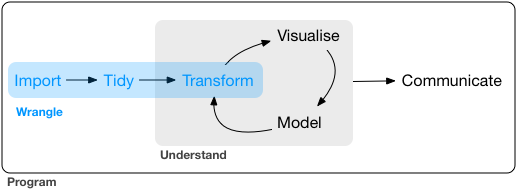
\includegraphics{figure/data-science-wrangle.png}
\caption{Data wrangling process {[}\textbf{Source:} \href{https://r4ds.had.co.nz/wrangle-intro.html}{Grolemund and Wickham (2018)}{]}}
\end{figure}

In this section, we will follow the steps of data wrangling as shown above.

\hypertarget{creating-data-in-r}{%
\section{\texorpdfstring{Creating Data in \textbf{R}}{Creating Data in R}}\label{creating-data-in-r}}

There are multiple ways of creating datasets in R. We can create individual variables and combine them using the \texttt{cbind} (column bind) command:

\begin{Shaded}
\begin{Highlighting}[]
\NormalTok{age <-}\StringTok{ }\KeywordTok{c}\NormalTok{(}\DecValTok{21}\NormalTok{, }\DecValTok{24}\NormalTok{, }\DecValTok{32}\NormalTok{, }\DecValTok{45}\NormalTok{, }\DecValTok{52}\NormalTok{)}
\NormalTok{salary <-}\StringTok{ }\KeywordTok{c}\NormalTok{(}\DecValTok{4500}\NormalTok{, }\DecValTok{3500}\NormalTok{, }\DecValTok{4100}\NormalTok{, }\DecValTok{4700}\NormalTok{, }\DecValTok{6000}\NormalTok{)}
\NormalTok{mydata <-}\StringTok{ }\KeywordTok{cbind}\NormalTok{(age, salary)}
\NormalTok{mydata}
\end{Highlighting}
\end{Shaded}

\begin{verbatim}
     age salary
[1,]  21   4500
[2,]  24   3500
[3,]  32   4100
[4,]  45   4700
[5,]  52   6000
\end{verbatim}

We can also create individual rows and combine them using the \texttt{rbind} (row bind) command (not practical if there are many rows):

\begin{Shaded}
\begin{Highlighting}[]
\NormalTok{person1 <-}\StringTok{ }\KeywordTok{c}\NormalTok{(}\DecValTok{21}\NormalTok{, }\DecValTok{4500}\NormalTok{)}
\NormalTok{person2 <-}\StringTok{ }\KeywordTok{c}\NormalTok{(}\DecValTok{24}\NormalTok{, }\DecValTok{3500}\NormalTok{)}
\NormalTok{person3 <-}\StringTok{ }\KeywordTok{c}\NormalTok{(}\DecValTok{32}\NormalTok{, }\DecValTok{4100}\NormalTok{)}
\NormalTok{person4 <-}\StringTok{ }\KeywordTok{c}\NormalTok{(}\DecValTok{45}\NormalTok{, }\DecValTok{4700}\NormalTok{)}
\NormalTok{person5 <-}\StringTok{ }\KeywordTok{c}\NormalTok{(}\DecValTok{52}\NormalTok{, }\DecValTok{6000}\NormalTok{)}

\NormalTok{mydata <-}\StringTok{ }\KeywordTok{rbind}\NormalTok{(person1, person2, person3, person4, person5)}
\NormalTok{mydata}
\end{Highlighting}
\end{Shaded}

\begin{verbatim}
        [,1] [,2]
person1   21 4500
person2   24 3500
person3   32 4100
person4   45 4700
person5   52 6000
\end{verbatim}

A better way to create datasets in \textbf{R} is to define variables within a data frame using the \texttt{data.frame} command.

\begin{Shaded}
\begin{Highlighting}[]
\NormalTok{mydata <-}\StringTok{ }\KeywordTok{data.frame}\NormalTok{(}\DataTypeTok{age =} \KeywordTok{c}\NormalTok{(}\DecValTok{21}\NormalTok{, }\DecValTok{24}\NormalTok{, }\DecValTok{32}\NormalTok{, }\DecValTok{45}\NormalTok{, }\DecValTok{52}\NormalTok{), }
                     \DataTypeTok{salary =} \KeywordTok{c}\NormalTok{(}\DecValTok{4500}\NormalTok{, }\DecValTok{3500}\NormalTok{, }\DecValTok{4100}\NormalTok{, }\DecValTok{4700}\NormalTok{, }\DecValTok{6000}\NormalTok{))}
\NormalTok{mydata}
\end{Highlighting}
\end{Shaded}

\begin{verbatim}
  age salary
1  21   4500
2  24   3500
3  32   4100
4  45   4700
5  52   6000
\end{verbatim}

Data frames in \textbf{R} are very convenient because many mathematical operations can be directly applied to a data frame or some columns (or rows) of a data frame. Once a data frame is defined in \textbf{R}, we can see its content using the \texttt{View} command (which open the data window) or the \texttt{head} command (which prints the first six rows of the data):

\begin{Shaded}
\begin{Highlighting}[]
\CommentTok{# To print the first six rows of a data frame}
\KeywordTok{head}\NormalTok{(mydata)}

\CommentTok{# To see the entire data in the view window}
\KeywordTok{View}\NormalTok{(mydata)}
\end{Highlighting}
\end{Shaded}

\hypertarget{importing-data-into-r}{%
\section{\texorpdfstring{Importing Data into \textbf{R}}{Importing Data into R}}\label{importing-data-into-r}}

We often save our data sets in convenient data formats, such as Excel, SPSS, or text files (.txt, .csv, .dat, etc.). \textbf{R} is capable of importing (i.e., reading) various data formats.

There are two ways to import a data set into \textbf{R}:

\begin{enumerate}
\def\labelenumi{\arabic{enumi}.}
\tightlist
\item
  By using the ``Import Dataset'' menu option in \textbf{RStudio}
\item
  By using a particular \textbf{R} command
\end{enumerate}

\hypertarget{method-1-using-rstudio}{%
\subsection{\texorpdfstring{Method 1: Using \textbf{RStudio}}{Method 1: Using RStudio}}\label{method-1-using-rstudio}}

\begin{figure}
\centering
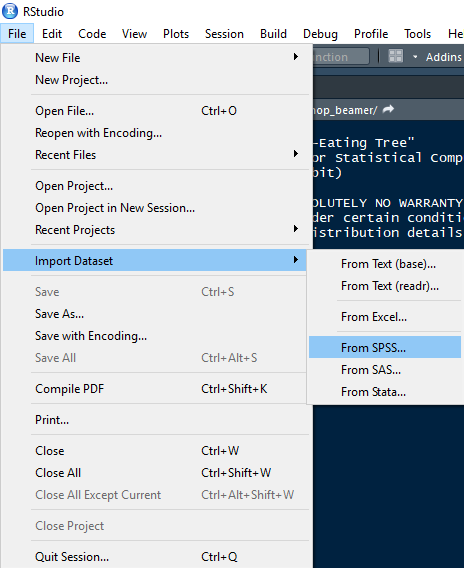
\includegraphics{figure/img8.png}
\caption{Importing a dataset using the \textbf{RStudio} menu}
\end{figure}

\hypertarget{importing-excel-files}{%
\subsubsection{Importing Excel Files}\label{importing-excel-files}}

\begin{itemize}
\tightlist
\item
  Browse for the file that you want to import
\item
  Give a name for the data set
\item
  Choose the sheet to be imported
\item
  ``First Row as Names'' if the variable names are in the first row of the file.
\end{itemize}

\begin{figure}
\centering
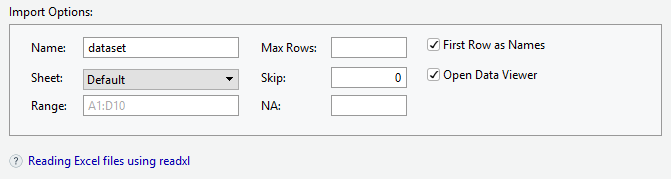
\includegraphics{figure/img9.png}
\caption{Importing Excel files}
\end{figure}

\hypertarget{importing-spss-files}{%
\subsubsection{Importing SPSS Files}\label{importing-spss-files}}

\begin{itemize}
\tightlist
\item
  Browse the file that you want to import
\item
  Give a name for the data set
\item
  Choose the SPSS data format (SAV)
\end{itemize}

\begin{figure}
\centering
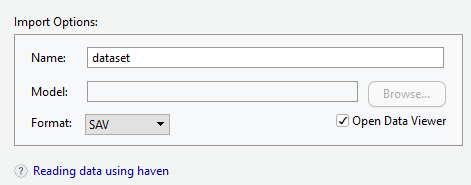
\includegraphics{figure/img10.png}
\caption{Importing SPSS files}
\end{figure}

\hypertarget{method-2-using-r-commands}{%
\subsection{\texorpdfstring{Method 2: Using \textbf{R} Commands}{Method 2: Using R Commands}}\label{method-2-using-r-commands}}

\textbf{R} has some built-in functions, such as \texttt{read.csv} and \texttt{read.table}. Also, there are \textbf{R} packages for importing specific data formats. For example, \texttt{foreign} for SPSS files and \texttt{xlsx} for Excel files. Here are some examples:

\textbf{Excel Files:}

\begin{Shaded}
\begin{Highlighting}[]
\CommentTok{# Install and activate the package first}
\KeywordTok{install.packages}\NormalTok{(}\StringTok{"xlsx"}\NormalTok{)}
\KeywordTok{library}\NormalTok{(}\StringTok{"xlsx"}\NormalTok{)}

\CommentTok{# Use read.xlsx to import an Excel file}
\NormalTok{my_excel_file <-}\StringTok{ }\KeywordTok{read.xlsx}\NormalTok{(}\StringTok{"path to the file/filename.xlsx"}\NormalTok{, }\DataTypeTok{sheetName =} \StringTok{"sheetname"}\NormalTok{)}
\end{Highlighting}
\end{Shaded}

\textbf{SPSS Files:}

\begin{Shaded}
\begin{Highlighting}[]
\CommentTok{# Install and activate the package first}
\KeywordTok{install.packages}\NormalTok{(}\StringTok{"foreign"}\NormalTok{)}
\KeywordTok{library}\NormalTok{(}\StringTok{"foreign"}\NormalTok{)}

\CommentTok{# Use read.xlsx to import an Excel file}
\NormalTok{my_spss_file <-}\StringTok{ }\KeywordTok{read.spss}\NormalTok{(}\StringTok{"path to the file/filename.sav"}\NormalTok{, }\DataTypeTok{to.data.frame =} \OtherTok{TRUE}\NormalTok{)}
\end{Highlighting}
\end{Shaded}

\textbf{Text Files:}

\begin{Shaded}
\begin{Highlighting}[]
\CommentTok{# No need to install any packages}
\CommentTok{# R has many built-in functions already}

\CommentTok{# A comma-separated-values file with a .csv extension}
\NormalTok{my_csv_file <-}\StringTok{ }\KeywordTok{read.csv}\NormalTok{(}\StringTok{"path to the file/filename.csv"}\NormalTok{, }\DataTypeTok{header =} \OtherTok{TRUE}\NormalTok{)}

\CommentTok{# A tab delimited text file with .txt extension}
\NormalTok{my_txt_file <-}\StringTok{ }\KeywordTok{read.table}\NormalTok{(}\StringTok{"path to the file/filename.txt"}\NormalTok{, }\DataTypeTok{header =} \OtherTok{TRUE}\NormalTok{, }\DataTypeTok{sep =} \StringTok{"}\CharTok{\textbackslash{}t}\StringTok{"}\NormalTok{)}
\end{Highlighting}
\end{Shaded}

Here we should note that:

\begin{itemize}
\tightlist
\item
  \texttt{header\ =\ TRUE} if the variable names are in the first row; otherwise, use \texttt{header\ =\ FALSE}
\item
  \texttt{sep="\textbackslash{}t"} for tab-separated files; \texttt{sep=","} for comma-separated files
\end{itemize}

\hypertarget{your-turn-2}{%
\subsection{Your Turn}\label{your-turn-2}}

Now we will import the \texttt{medical} dataset into \textbf{R}. The dataset comes from a clinical study. Patients with no primary care physician were randomized to receive a multidisciplinary assessment and a brief motivational intervention, with the goal of linking them to primary medical care. You can find the details in ``Codebook for the medical Dataset'' in your folder.

We have both Excel and text (with .csv extension) versions of the same file.

\begin{enumerate}
\def\labelenumi{\arabic{enumi}.}
\item
  Import the file \texttt{medical\_EXCEL} by using the ``Import Dataset'' menu option and name it as \texttt{medical} or import the file \texttt{medical\_CSV} by using the \texttt{read.csv} command and name it as \texttt{medical}
\item
  Once the data file is successfully important, run the following code to see the first six rows of the data:
\end{enumerate}

\begin{Shaded}
\begin{Highlighting}[]
\KeywordTok{head}\NormalTok{(medical)}
\end{Highlighting}
\end{Shaded}

You should be able to see the output below:

\begin{verbatim}
  id age    sex  race homeless substance avg_drinks max_drinks suicidal
1  1  37   male black   housed   cocaine         13         26      yes
2  2  37   male white homeless   alcohol         56         62      yes
3  3  26   male black   housed    heroin          0          0       no
4  4  39 female white   housed    heroin          5          5       no
5  5  32   male black homeless   cocaine         10         13       no
6  6  47 female black   housed   cocaine          4          4       no
  treat physical1 mental1 depression1 physical2 mental2 depression2
1   yes     58.41  25.112          49     54.23   52.23           7
2   yes     36.04  26.670          30     59.56   41.73          11
3    no     74.81   6.763          39     58.46   56.77          14
4    no     61.93  43.968          15     46.61   14.66          44
5    no     37.35  21.676          39     31.42   40.67          26
6   yes     46.48  55.509           6     43.20   50.06          23
\end{verbatim}

\hypertarget{understanding-the-data}{%
\section{Understanding the Data}\label{understanding-the-data}}

After we import a dataset into \textbf{R}, we can quickly check a few things to understand our dataset better:

\begin{itemize}
\tightlist
\item
  To see the number of rows in the data:
\end{itemize}

\begin{Shaded}
\begin{Highlighting}[]
\KeywordTok{nrow}\NormalTok{(medical)}
\end{Highlighting}
\end{Shaded}

\begin{verbatim}
[1] 246
\end{verbatim}

\begin{itemize}
\tightlist
\item
  To see the number of columns in the data:
\end{itemize}

\begin{Shaded}
\begin{Highlighting}[]
\KeywordTok{ncol}\NormalTok{(medical)}
\end{Highlighting}
\end{Shaded}

\begin{verbatim}
[1] 16
\end{verbatim}

\begin{itemize}
\tightlist
\item
  To see its dimensions all together:
\end{itemize}

\begin{Shaded}
\begin{Highlighting}[]
\KeywordTok{dim}\NormalTok{(medical)}
\end{Highlighting}
\end{Shaded}

\begin{verbatim}
[1] 246  16
\end{verbatim}

\begin{itemize}
\tightlist
\item
  To see all of the variable names in the data:
\end{itemize}

\begin{Shaded}
\begin{Highlighting}[]
\KeywordTok{names}\NormalTok{(medical)}
\end{Highlighting}
\end{Shaded}

\begin{verbatim}
 [1] "id"          "age"         "sex"         "race"        "homeless"   
 [6] "substance"   "avg_drinks"  "max_drinks"  "suicidal"    "treat"      
[11] "physical1"   "mental1"     "depression1" "physical2"   "mental2"    
[16] "depression2"
\end{verbatim}

\begin{itemize}
\tightlist
\item
  To see the structure of the entire dataset:
\end{itemize}

\begin{Shaded}
\begin{Highlighting}[]
\KeywordTok{str}\NormalTok{(medical)}
\end{Highlighting}
\end{Shaded}

\begin{verbatim}
'data.frame':   246 obs. of  16 variables:
 $ id         : int  1 2 3 4 5 6 8 9 10 12 ...
 $ age        : int  37 37 26 39 32 47 28 50 39 58 ...
 $ sex        : chr  "male" "male" "male" "female" ...
 $ race       : chr  "black" "white" "black" "white" ...
 $ homeless   : chr  "housed" "homeless" "housed" "housed" ...
 $ substance  : chr  "cocaine" "alcohol" "heroin" "heroin" ...
 $ avg_drinks : int  13 56 0 5 10 4 12 71 20 13 ...
 $ max_drinks : int  26 62 0 5 13 4 24 129 27 13 ...
 $ suicidal   : chr  "yes" "yes" "no" "no" ...
 $ treat      : chr  "yes" "yes" "no" "no" ...
 $ physical1  : num  58.4 36 74.8 61.9 37.3 ...
 $ mental1    : num  25.11 26.67 6.76 43.97 21.68 ...
 $ depression1: int  49 30 39 15 39 6 32 50 46 49 ...
 $ physical2  : num  54.2 59.6 58.5 46.6 31.4 ...
 $ mental2    : num  52.2 41.7 56.8 14.7 40.7 ...
 $ depression2: int  7 11 14 44 26 23 18 33 37 8 ...
\end{verbatim}

\hypertarget{indexing}{%
\section{Indexing}\label{indexing}}

In \textbf{R}, each row and column is indexed by the position they appear in the data. \textbf{R} uses square brackets for indexing. Within the square brackets, the first number shows the row number(s) and the second number shows the column(s). To call a particular column (i.e., variables) or a particular row (i.e., persons), we can use the following structure: \texttt{data{[}row,\ col{]}}

For example, if we want to see the second variable for the fifth person in the \texttt{medical} dataset:

\begin{Shaded}
\begin{Highlighting}[]
\NormalTok{medical[}\DecValTok{5}\NormalTok{, }\DecValTok{2}\NormalTok{]}
\end{Highlighting}
\end{Shaded}

\begin{verbatim}
[1] 32
\end{verbatim}

Or, if we want to see the first three variables for the first five persons:

\begin{Shaded}
\begin{Highlighting}[]
\NormalTok{medical[}\DecValTok{1}\OperatorTok{:}\DecValTok{5}\NormalTok{, }\DecValTok{1}\OperatorTok{:}\DecValTok{3}\NormalTok{]}
\end{Highlighting}
\end{Shaded}

\begin{verbatim}
  id age    sex
1  1  37   male
2  2  37   male
3  3  26   male
4  4  39 female
5  5  32   male
\end{verbatim}

Instead of \texttt{medical{[}1:5,\ 1:3{]}}, we could also do:

\begin{Shaded}
\begin{Highlighting}[]
\NormalTok{medical[}\KeywordTok{c}\NormalTok{(}\DecValTok{1}\NormalTok{, }\DecValTok{2}\NormalTok{, }\DecValTok{3}\NormalTok{, }\DecValTok{4}\NormalTok{, }\DecValTok{5}\NormalTok{), }\KeywordTok{c}\NormalTok{(}\DecValTok{1}\NormalTok{, }\DecValTok{2}\NormalTok{, }\DecValTok{3}\NormalTok{)]}
\end{Highlighting}
\end{Shaded}

\begin{verbatim}
  id age    sex
1  1  37   male
2  2  37   male
3  3  26   male
4  4  39 female
5  5  32   male
\end{verbatim}

or

\begin{Shaded}
\begin{Highlighting}[]
\NormalTok{medical[}\KeywordTok{c}\NormalTok{(}\DecValTok{1}\NormalTok{, }\DecValTok{2}\NormalTok{, }\DecValTok{3}\NormalTok{, }\DecValTok{4}\NormalTok{, }\DecValTok{5}\NormalTok{), }\KeywordTok{c}\NormalTok{(}\StringTok{"id"}\NormalTok{, }\StringTok{"age"}\NormalTok{, }\StringTok{"sex"}\NormalTok{)]}
\end{Highlighting}
\end{Shaded}

\begin{verbatim}
  id age    sex
1  1  37   male
2  2  37   male
3  3  26   male
4  4  39 female
5  5  32   male
\end{verbatim}

A common way of indexing variables (i.e., columns) in \textbf{R} is to use the dollar sign with a variable name from a data frame. For example, we can select the age variable as follows:

\begin{Shaded}
\begin{Highlighting}[]
\NormalTok{medical}\OperatorTok{$}\NormalTok{age}
\end{Highlighting}
\end{Shaded}

This would print all the values for age in the \texttt{medical} dataset. We can also preview a particular variable using the \texttt{head} function.

\begin{Shaded}
\begin{Highlighting}[]
\KeywordTok{head}\NormalTok{(medical}\OperatorTok{$}\NormalTok{age)}
\end{Highlighting}
\end{Shaded}

\begin{verbatim}
[1] 37 37 26 39 32 47
\end{verbatim}

Using a particular variable, we can also see the values for some rows in the data. For example, let's print the age variable for the 10th to 15th rows in the \texttt{medical} dataset.

\begin{Shaded}
\begin{Highlighting}[]
\NormalTok{medical}\OperatorTok{$}\NormalTok{age[}\DecValTok{10}\OperatorTok{:}\DecValTok{15}\NormalTok{]}

\CommentTok{#or}

\NormalTok{medical}\OperatorTok{$}\NormalTok{age[}\KeywordTok{c}\NormalTok{(}\DecValTok{10}\NormalTok{, }\DecValTok{11}\NormalTok{, }\DecValTok{12}\NormalTok{, }\DecValTok{13}\NormalTok{, }\DecValTok{14}\NormalTok{, }\DecValTok{15}\NormalTok{)]}
\end{Highlighting}
\end{Shaded}

Note that now the brackets don't need a comma inside as we had before. This is because we have already selected a variable (age) and so \textbf{R} knows that we now refer to rows when we type any values inside the brackets.

\hypertarget{subsetting}{%
\section{Subsetting}\label{subsetting}}

Now assume that we want to create a new dataset with only females from the \texttt{medical} dataset. Although we can take this subset in many ways, the following three are the easiest ways:

\begin{enumerate}
\def\labelenumi{\arabic{enumi}.}
\tightlist
\item
  Using the indexing idea to refer to certain variables:
\end{enumerate}

\begin{Shaded}
\begin{Highlighting}[]
\NormalTok{medical_female <-}\StringTok{ }\NormalTok{medical[medical}\OperatorTok{$}\NormalTok{sex }\OperatorTok{==}\StringTok{ "female"}\NormalTok{, ]}
\KeywordTok{head}\NormalTok{(medical_female)}
\end{Highlighting}
\end{Shaded}

\begin{verbatim}
   id age    sex     race homeless substance avg_drinks max_drinks
4   4  39 female    white   housed    heroin          5          5
6   6  47 female    black   housed   cocaine          4          4
8   9  50 female    white homeless   alcohol         71        129
10 12  58 female    black   housed   alcohol         13         13
14 17  28 female hispanic homeless    heroin          0          0
17 20  27 female    white   housed    heroin          9         24
   suicidal treat physical1 mental1 depression1 physical2 mental2
4        no    no     61.93   43.97          15     46.61   14.66
6        no   yes     46.48   55.51           6     43.20   50.06
8        no    no     38.27   22.03          50     45.56   28.88
10       no    no     41.93   13.38          49     52.96   51.45
14      yes   yes     44.78   29.80          35     52.69   46.59
17      yes   yes     37.45   15.46          52     61.40   41.53
   depression2
4           44
6           23
8           33
10           8
14          19
17          15
\end{verbatim}

We set the criterion \texttt{medical\$sex\ ==\ "female"} before the comma to make a selection for rows and there is nothing after comma in the bracket because we want to keep all the variables in the dataset. This method is handy for simple selections but it gets complicated when we have multiple subsetting criteria. See the example below with two criteria:

\begin{Shaded}
\begin{Highlighting}[]
\NormalTok{medical_female_}\DecValTok{40}\NormalTok{ <-}\StringTok{ }\NormalTok{medical[medical}\OperatorTok{$}\NormalTok{sex }\OperatorTok{==}\StringTok{ "female"} \OperatorTok{&}\StringTok{ }\NormalTok{medical}\OperatorTok{$}\NormalTok{age }\OperatorTok{>}\StringTok{ }\DecValTok{40}\NormalTok{, ]}
\end{Highlighting}
\end{Shaded}

\begin{enumerate}
\def\labelenumi{\arabic{enumi}.}
\setcounter{enumi}{1}
\tightlist
\item
  Using the \texttt{subset} function in base \textbf{R}:
\end{enumerate}

\begin{Shaded}
\begin{Highlighting}[]
\NormalTok{medical_female <-}\StringTok{ }\KeywordTok{subset}\NormalTok{(medical, sex }\OperatorTok{==}\StringTok{ "female"}\NormalTok{)}
\KeywordTok{head}\NormalTok{(medical_female)}
\end{Highlighting}
\end{Shaded}

\begin{verbatim}
   id age    sex     race homeless substance avg_drinks max_drinks
4   4  39 female    white   housed    heroin          5          5
6   6  47 female    black   housed   cocaine          4          4
8   9  50 female    white homeless   alcohol         71        129
10 12  58 female    black   housed   alcohol         13         13
14 17  28 female hispanic homeless    heroin          0          0
17 20  27 female    white   housed    heroin          9         24
   suicidal treat physical1 mental1 depression1 physical2 mental2
4        no    no     61.93   43.97          15     46.61   14.66
6        no   yes     46.48   55.51           6     43.20   50.06
8        no    no     38.27   22.03          50     45.56   28.88
10       no    no     41.93   13.38          49     52.96   51.45
14      yes   yes     44.78   29.80          35     52.69   46.59
17      yes   yes     37.45   15.46          52     61.40   41.53
   depression2
4           44
6           23
8           33
10           8
14          19
17          15
\end{verbatim}

\begin{enumerate}
\def\labelenumi{\arabic{enumi}.}
\setcounter{enumi}{2}
\tightlist
\item
  Using the \texttt{filter} function from the \texttt{dplyr} package (an amazing package for data wrangling):
\end{enumerate}

\begin{Shaded}
\begin{Highlighting}[]
\CommentTok{# Install and activate the package first}
\KeywordTok{install.packages}\NormalTok{(}\StringTok{"dplyr"}\NormalTok{)}
\KeywordTok{library}\NormalTok{(}\StringTok{"dplyr"}\NormalTok{)}

\NormalTok{medical_female <-}\StringTok{ }\KeywordTok{filter}\NormalTok{(medical, sex }\OperatorTok{==}\StringTok{ "female"}\NormalTok{)}

\KeywordTok{head}\NormalTok{(medical_female)}
\end{Highlighting}
\end{Shaded}

\begin{Shaded}
\begin{Highlighting}[]
\KeywordTok{head}\NormalTok{(medical_female)}
\end{Highlighting}
\end{Shaded}

\begin{verbatim}
  id age    sex     race homeless substance avg_drinks max_drinks suicidal
1  4  39 female    white   housed    heroin          5          5       no
2  6  47 female    black   housed   cocaine          4          4       no
3  9  50 female    white homeless   alcohol         71        129       no
4 12  58 female    black   housed   alcohol         13         13       no
5 17  28 female hispanic homeless    heroin          0          0      yes
6 20  27 female    white   housed    heroin          9         24      yes
  treat physical1 mental1 depression1 physical2 mental2 depression2
1    no     61.93   43.97          15     46.61   14.66          44
2   yes     46.48   55.51           6     43.20   50.06          23
3    no     38.27   22.03          50     45.56   28.88          33
4    no     41.93   13.38          49     52.96   51.45           8
5   yes     44.78   29.80          35     52.69   46.59          19
6   yes     37.45   15.46          52     61.40   41.53          15
\end{verbatim}

We can also create a new dataset by subsetting based on multiple criteria and selecting only some variables from our original data. Let's assume that we want to select participants who are female and 40 years old or older. Also, we only want to keep the following variables in the dataset: id, age, sex, substance.

\begin{enumerate}
\def\labelenumi{\arabic{enumi}.}
\tightlist
\item
  Using the \texttt{subset} function in base \textbf{R}:
\end{enumerate}

\begin{Shaded}
\begin{Highlighting}[]
\NormalTok{medical_f40 <-}\StringTok{ }\KeywordTok{subset}\NormalTok{(medical, sex }\OperatorTok{==}\StringTok{ "female"} \OperatorTok{&}\StringTok{ }\NormalTok{age }\OperatorTok{>=}\StringTok{ }\DecValTok{40}\NormalTok{, }
                      \DataTypeTok{select =} \KeywordTok{c}\NormalTok{(}\StringTok{"id"}\NormalTok{, }\StringTok{"age"}\NormalTok{, }\StringTok{"sex"}\NormalTok{, }\StringTok{"substance"}\NormalTok{))}

\KeywordTok{head}\NormalTok{(medical_f40)}
\end{Highlighting}
\end{Shaded}

\begin{verbatim}
   id age    sex substance
6   6  47 female   cocaine
8   9  50 female   alcohol
10 12  58 female   alcohol
21 27  48 female   cocaine
51 65  41 female   alcohol
56 71  40 female   alcohol
\end{verbatim}

\begin{enumerate}
\def\labelenumi{\arabic{enumi}.}
\setcounter{enumi}{1}
\tightlist
\item
  Using the \texttt{filter} and \texttt{select} functions from the \texttt{dplyr} package
\end{enumerate}

\begin{Shaded}
\begin{Highlighting}[]
\NormalTok{medical_f40 <-}\StringTok{ }\NormalTok{medical }\OperatorTok\StringTok{ }
\StringTok{  }\KeywordTok{filter}\NormalTok{(sex }\OperatorTok{==}\StringTok{ "female"}\NormalTok{, age }\OperatorTok{>=}\StringTok{ }\DecValTok{40}\NormalTok{) }\OperatorTok
\StringTok{  }\KeywordTok{select}\NormalTok{(id, age, sex, substance)}

\KeywordTok{head}\NormalTok{(medical_f40)}
\end{Highlighting}
\end{Shaded}

\begin{verbatim}
  id age    sex substance
1  6  47 female   cocaine
2  9  50 female   alcohol
3 12  58 female   alcohol
4 27  48 female   cocaine
5 65  41 female   alcohol
6 71  40 female   alcohol
\end{verbatim}

Here I demonstrate the \texttt{\%\textgreater{}\%} operator called the pipe. This operator forwards a value, or the result of an expression, into the next function call/expression. This way we can simplify the code without creating many intermediate datasets (see \url{https://uc-r.github.io/pipe} for more details on the pipe).

Here are most common operators for subsetting:

\begin{itemize}
\tightlist
\item
  \texttt{\textless{}} Less than
\item
  \texttt{\textgreater{}} Greater than
\item
  \texttt{==} Equal to
\item
  \texttt{\textless{}=} Less than or equal to
\item
  \texttt{\textgreater{}=} Greater than or equal to
\item
  \texttt{!=} Not equal to
\item
  \texttt{\%in\%} Group membership
\item
  \texttt{\&} And
\item
  \texttt{\textbar{}} Or
\item
  \texttt{is.na} Is missing (NA).
\item
  \texttt{!is.na} Is not missing (NA)
\end{itemize}

\hypertarget{other-data-manipulation-tools}{%
\section{Other Data Manipulation Tools}\label{other-data-manipulation-tools}}

Here I will mention the other key functions from the \texttt{dplyr} package. These functions solve the vast majority of data manipulation challenges:

\begin{itemize}
\tightlist
\item
  \texttt{arrange}: Reorder data based on values of variables
\item
  \texttt{mutate}: Create new variables
\item
  \texttt{summarise}: Summarize data by functions of choice
\end{itemize}

\textbf{Arrange:}

\begin{Shaded}
\begin{Highlighting}[]
\CommentTok{# Reorder the data by age}
\NormalTok{medical_f40 <-}\StringTok{ }\KeywordTok{arrange}\NormalTok{(medical_f40, age)}

\CommentTok{# Let's see if the ordering worked}
\KeywordTok{head}\NormalTok{(medical_f40)}
\end{Highlighting}
\end{Shaded}

\begin{verbatim}
   id age    sex substance
1  71  40 female   alcohol
2  65  41 female   alcohol
3  75  41 female    heroin
4 121  42 female   cocaine
5 465  42 female   alcohol
6 364  43 female    heroin
\end{verbatim}

\begin{Shaded}
\begin{Highlighting}[]
\CommentTok{# Reorder the data by age in descending order}
\NormalTok{medical_f40 <-}\StringTok{ }\KeywordTok{arrange}\NormalTok{(medical_f40, }\KeywordTok{desc}\NormalTok{(age))}

\CommentTok{# Let's see if the ordering worked}
\KeywordTok{head}\NormalTok{(medical_f40)}
\end{Highlighting}
\end{Shaded}

\begin{verbatim}
   id age    sex substance
1  12  58 female   alcohol
2 181  57 female   alcohol
3 264  55 female    heroin
4   9  50 female   alcohol
5 134  50 female   alcohol
6  27  48 female   cocaine
\end{verbatim}

\textbf{Mutate:}

\begin{Shaded}
\begin{Highlighting}[]
\CommentTok{# Create a new variable based on age}
\NormalTok{medical_f40 <-}\StringTok{ }\NormalTok{medical_f40 }\OperatorTok
\StringTok{  }\KeywordTok{mutate}\NormalTok{(}\DataTypeTok{age2 =} \KeywordTok{ifelse}\NormalTok{(age }\OperatorTok{<}\StringTok{ }\DecValTok{45}\NormalTok{, }\StringTok{"Younger than 45"}\NormalTok{, }\StringTok{"45 or older"}\NormalTok{))}

\CommentTok{# Let's see if the ordering worked}
\KeywordTok{head}\NormalTok{(medical_f40)}
\end{Highlighting}
\end{Shaded}

\begin{verbatim}
   id age    sex substance        age2
1  12  58 female   alcohol 45 or older
2 181  57 female   alcohol 45 or older
3 264  55 female    heroin 45 or older
4   9  50 female   alcohol 45 or older
5 134  50 female   alcohol 45 or older
6  27  48 female   cocaine 45 or older
\end{verbatim}

We will use the \texttt{summarise} function in the next section.

\hypertarget{your-turn-3}{%
\subsection{Your Turn}\label{your-turn-3}}

\begin{enumerate}
\def\labelenumi{\arabic{enumi}.}
\item
  Using the medical data, create a subset where the patients:

  \begin{itemize}
  \tightlist
  \item
    are older than 30 years old: \texttt{age\ \textgreater{}\ 30}
  \item
    are female: \texttt{sex\ ==\ "female"}
  \item
    are not homeless: \texttt{homeless\ !=\ "homeless"}
  \end{itemize}
\end{enumerate}

and save this data as \texttt{medical\_example}. You can use either \texttt{subset} or \texttt{filter} for this task.

\begin{enumerate}
\def\labelenumi{\arabic{enumi}.}
\setcounter{enumi}{1}
\item
  Use the \texttt{dim} function to see how many rows you have in the new data
\item
  Sort this new dataset by age in descending order
\item
  Use the \texttt{head} function to preview the final dataset
\end{enumerate}

\hypertarget{part3}{%
\chapter{Descriptive Statistics}\label{part3}}

\hypertarget{quick-summary}{%
\section{Quick Summary}\label{quick-summary}}

The easiest way to get a quick summary of a dataset in \textbf{R} is to the \texttt{summary(\ )} function. This function provides the min and max, mean, median, and first and third quartiles for the entire dataset or variables that we select. Let's take a look at the summary table for the \texttt{medical} dataset.

\begin{Shaded}
\begin{Highlighting}[]
\KeywordTok{summary}\NormalTok{(medical)}
\end{Highlighting}
\end{Shaded}

\begin{verbatim}
       id             age           sex                race          
 Min.   :  1.0   Min.   :20.0   Length:246         Length:246        
 1st Qu.: 82.5   1st Qu.:31.0   Class :character   Class :character  
 Median :210.5   Median :35.0   Mode  :character   Mode  :character  
 Mean   :216.3   Mean   :36.3                                        
 3rd Qu.:346.8   3rd Qu.:41.0                                        
 Max.   :469.0   Max.   :60.0                                        
   homeless          substance           avg_drinks      max_drinks   
 Length:246         Length:246         Min.   :  0.0   Min.   :  0.0  
 Class :character   Class :character   1st Qu.:  2.0   1st Qu.:  3.0  
 Mode  :character   Mode  :character   Median : 12.0   Median : 13.0  
                                       Mean   : 17.1   Mean   : 24.1  
                                       3rd Qu.: 24.0   3rd Qu.: 32.0  
                                       Max.   :142.0   Max.   :184.0  
   suicidal            treat             physical1       mental1     
 Length:246         Length:246         Min.   :14.1   Min.   : 6.76  
 Class :character   Class :character   1st Qu.:38.3   1st Qu.:21.95  
 Mode  :character   Mode  :character   Median :48.9   Median :29.15  
                                       Mean   :47.5   Mean   :31.68  
                                       3rd Qu.:56.5   3rd Qu.:40.62  
                                       Max.   :74.8   Max.   :60.54  
  depression1     physical2       mental2       depression2  
 Min.   : 1.0   Min.   :19.7   Min.   : 6.68   Min.   : 0.0  
 1st Qu.:25.2   1st Qu.:42.8   1st Qu.:30.21   1st Qu.:11.0  
 Median :34.0   Median :53.3   Median :42.44   Median :22.0  
 Mean   :32.6   Mean   :50.2   Mean   :40.98   Mean   :22.7  
 3rd Qu.:41.0   3rd Qu.:58.2   3rd Qu.:52.73   3rd Qu.:34.8  
 Max.   :57.0   Max.   :71.4   Max.   :69.94   Max.   :56.0  
\end{verbatim}

\textbf{R} often knows which variables are numerical (i.e., quantitative) and which variables are characters (i.e., qualitative). In the output above, we see a bunch of summary statistics for each variable -- though some don't make sense such as the id variable. For character variables, we only see the length value -- which is the number of rows for these variables.

We can also select either a single variable or a set of variables and see the summary table only for the selected variables:

\begin{Shaded}
\begin{Highlighting}[]
\CommentTok{# Summary for age}
\KeywordTok{summary}\NormalTok{(medical}\OperatorTok{$}\NormalTok{age)}
\end{Highlighting}
\end{Shaded}

\begin{verbatim}
   Min. 1st Qu.  Median    Mean 3rd Qu.    Max. 
   20.0    31.0    35.0    36.3    41.0    60.0 
\end{verbatim}

\begin{Shaded}
\begin{Highlighting}[]
\CommentTok{# Summary for age, average drinks, and maximum drinks}
\KeywordTok{summary}\NormalTok{(medical[,}\KeywordTok{c}\NormalTok{(}\StringTok{"age"}\NormalTok{, }\StringTok{"avg_drinks"}\NormalTok{, }\StringTok{"max_drinks"}\NormalTok{)])}
\end{Highlighting}
\end{Shaded}

\begin{verbatim}
      age         avg_drinks      max_drinks   
 Min.   :20.0   Min.   :  0.0   Min.   :  0.0  
 1st Qu.:31.0   1st Qu.:  2.0   1st Qu.:  3.0  
 Median :35.0   Median : 12.0   Median : 13.0  
 Mean   :36.3   Mean   : 17.1   Mean   : 24.1  
 3rd Qu.:41.0   3rd Qu.: 24.0   3rd Qu.: 32.0  
 Max.   :60.0   Max.   :142.0   Max.   :184.0  
\end{verbatim}

\hypertarget{frequency-tables}{%
\section{Frequency Tables}\label{frequency-tables}}

Another handy function in base \textbf{R} is \texttt{table} which tabulates the data and creates frequency tables for variables. If he variable is character, it will show the frequency of each level; if the variable is numerical, it will show the frequency of each value.

\begin{Shaded}
\begin{Highlighting}[]
\CommentTok{# Frequency tables for homeless status and sex}
\KeywordTok{table}\NormalTok{(medical}\OperatorTok{$}\NormalTok{homeless)}
\end{Highlighting}
\end{Shaded}

\begin{verbatim}

homeless   housed 
     118      128 
\end{verbatim}

\begin{Shaded}
\begin{Highlighting}[]
\KeywordTok{table}\NormalTok{(medical}\OperatorTok{$}\NormalTok{sex)}
\end{Highlighting}
\end{Shaded}

\begin{verbatim}

female   male 
    57    189 
\end{verbatim}

\begin{Shaded}
\begin{Highlighting}[]
\CommentTok{# Frequency table for age}
\KeywordTok{table}\NormalTok{(medical}\OperatorTok{$}\NormalTok{age)}
\end{Highlighting}
\end{Shaded}

\begin{verbatim}

20 22 23 24 25 26 27 28 29 30 31 32 33 34 35 36 37 38 39 40 41 42 43 44 45 
 2  7  3  4  2  6  8  9  4 12  7 19 14 11 16 11 16  6 16  5  8  7 10  3  6 
46 47 48 49 50 51 53 54 55 56 57 58 60 
 2 10  5  4  2  1  2  1  2  1  1  2  1 
\end{verbatim}

The output is kind of messy. The first row shows the age values and the second row shows how many times those values appear in the dataset. Let's reformat our frequency table into a more readable format.

\begin{Shaded}
\begin{Highlighting}[]
\NormalTok{age_table <-}\StringTok{ }\KeywordTok{as.data.frame}\NormalTok{(}\KeywordTok{table}\NormalTok{(medical}\OperatorTok{$}\NormalTok{age))}
\KeywordTok{head}\NormalTok{(age_table)}
\end{Highlighting}
\end{Shaded}

\begin{verbatim}
  Var1 Freq
1   20    2
2   22    7
3   23    3
4   24    4
5   25    2
6   26    6
\end{verbatim}

We can rename the columns with better names using the \texttt{colnames(\ )} function.

\begin{Shaded}
\begin{Highlighting}[]
\KeywordTok{colnames}\NormalTok{(age_table) <-}\StringTok{ }\KeywordTok{c}\NormalTok{(}\StringTok{"Age"}\NormalTok{, }\StringTok{"Frequency"}\NormalTok{)}
\KeywordTok{head}\NormalTok{(age_table)}
\end{Highlighting}
\end{Shaded}

\begin{verbatim}
  Age Frequency
1  20         2
2  22         7
3  23         3
4  24         4
5  25         2
6  26         6
\end{verbatim}

Sometimes these raw freqency values are hard to interpret. Therefore, we may prefer to have proportions or percentages rather than actual frequency values. For this task, we need to use \texttt{prop.table}. Let's see the proportion of male and female participants in the data.

\begin{Shaded}
\begin{Highlighting}[]
\CommentTok{# Proportions}
\KeywordTok{prop.table}\NormalTok{(}\KeywordTok{table}\NormalTok{(medical}\OperatorTok{$}\NormalTok{sex))}
\end{Highlighting}
\end{Shaded}

\begin{verbatim}

female   male 
0.2317 0.7683 
\end{verbatim}

\begin{Shaded}
\begin{Highlighting}[]
\CommentTok{# Percentages}
\KeywordTok{prop.table}\NormalTok{(}\KeywordTok{table}\NormalTok{(medical}\OperatorTok{$}\NormalTok{sex))}\OperatorTok{*}\DecValTok{100}
\end{Highlighting}
\end{Shaded}

\begin{verbatim}

female   male 
 23.17  76.83 
\end{verbatim}

\begin{Shaded}
\begin{Highlighting}[]
\CommentTok{# Percentages rounded (no decimal points)}
\KeywordTok{round}\NormalTok{(}\KeywordTok{prop.table}\NormalTok{(}\KeywordTok{table}\NormalTok{(medical}\OperatorTok{$}\NormalTok{sex))}\OperatorTok{*}\DecValTok{100}\NormalTok{, }\DecValTok{0}\NormalTok{)}
\end{Highlighting}
\end{Shaded}

\begin{verbatim}

female   male 
    23     77 
\end{verbatim}

We can also use the \texttt{table} function for cross-tabulation. For example, if we want to see the number of homeless and housed patients by sex:

\begin{Shaded}
\begin{Highlighting}[]
\CommentTok{# Frequencies}
\KeywordTok{table}\NormalTok{(medical}\OperatorTok{$}\NormalTok{homeless, medical}\OperatorTok{$}\NormalTok{sex)}
\end{Highlighting}
\end{Shaded}

\begin{verbatim}
          
           female male
  homeless     22   96
  housed       35   93
\end{verbatim}

\begin{Shaded}
\begin{Highlighting}[]
\CommentTok{# Proportions}
\KeywordTok{prop.table}\NormalTok{(}\KeywordTok{table}\NormalTok{(medical}\OperatorTok{$}\NormalTok{homeless, medical}\OperatorTok{$}\NormalTok{sex))}
\end{Highlighting}
\end{Shaded}

\begin{verbatim}
          
            female    male
  homeless 0.08943 0.39024
  housed   0.14228 0.37805
\end{verbatim}

\begin{Shaded}
\begin{Highlighting}[]
\CommentTok{# Percentages}
\KeywordTok{prop.table}\NormalTok{(}\KeywordTok{table}\NormalTok{(medical}\OperatorTok{$}\NormalTok{homeless, medical}\OperatorTok{$}\NormalTok{sex))}\OperatorTok{*}\DecValTok{100}
\end{Highlighting}
\end{Shaded}

\begin{verbatim}
          
           female   male
  homeless  8.943 39.024
  housed   14.228 37.805
\end{verbatim}

\begin{Shaded}
\begin{Highlighting}[]
\CommentTok{# Percentages rounded to the 2nd decimal point}
\KeywordTok{round}\NormalTok{(}\KeywordTok{prop.table}\NormalTok{(}\KeywordTok{table}\NormalTok{(medical}\OperatorTok{$}\NormalTok{homeless, medical}\OperatorTok{$}\NormalTok{sex))}\OperatorTok{*}\DecValTok{100}\NormalTok{, }\DecValTok{2}\NormalTok{)}
\end{Highlighting}
\end{Shaded}

\begin{verbatim}
          
           female  male
  homeless   8.94 39.02
  housed    14.23 37.80
\end{verbatim}

\hypertarget{your-turn-4}{%
\subsection{Your Turn}\label{your-turn-4}}

Use the \texttt{table} function to create a cross tabulation for \texttt{race} and \texttt{substance}. We want to see the percentages with no decimal points. Which group is the largest and which group is the smallest based on their percentages?

\hypertarget{central-tendency-and-dispersion}{%
\section{Central Tendency and Dispersion}\label{central-tendency-and-dispersion}}

Central tendency refers to indices or measures that gives us an idea about the center of the data. Typical central tendency measures are:

\begin{itemize}
\tightlist
\item
  \textbf{Mean}: The sum of the values for a given variable divided by the number of values (\(n\)). Mean is typically denoted by \(\bar{X}\) (read as ``x bar'') or simply \(M\). We can find the mean as:
\end{itemize}

\[\bar{X} = \frac{X_1 + X_2 + X_3 + ...+ X_n}{n}.\]

\begin{itemize}
\tightlist
\item
  \textbf{Median}: The middle value for a given variable when the values are sorted from smallest to largest.
\end{itemize}

Dispersion refers to statistics that tell us how dispersed or spread out the values of a variable are. Typical dispersion measures are:

\begin{itemize}
\tightlist
\item
  \textbf{Standard deviation}: A typical difference (deviation) between a particular value and the mean of a variable. Standard deviation is denoted by \(\sigma\) (read as ``sigma''). We can find the standard deviation as:
\end{itemize}

\[\sigma = \sqrt{\frac{(X_1-\bar{X})^2+(X_2-\bar{X})^2+...+(X_n-\bar{X})^2}{n}}\]

\begin{itemize}
\item
  \textbf{Variance}: Variance is the squared value of standard deviation, \(\sigma^2\).
\item
  \textbf{Quantiles}: If we divide a cumulative frequency curve into quarters, the value at the lower quarter is referred to as the lower quartile, the value at the middle gives the median and the value at the upper quarter is the upper quartile.
\item
  \textbf{Range}: Difference between the biggest value and the smallest value of a variable.
\item
  \textbf{Interquartile range (IQR)}: Like the range, but instead of calculating the difference between the biggest and smallest values, it calculates the difference between the 25th quantile and the 75th quantile.
\end{itemize}

In \textbf{R}, we can calculate all of these statistics quite simply. A critical point is that if the variable has missing values, then these statistics cannot be computed. Therefore, we need to add \texttt{na.rm\ =\ TRUE} inside the functions. Let's try the variable \texttt{age}.

\begin{Shaded}
\begin{Highlighting}[]
\CommentTok{# Mean}
\KeywordTok{mean}\NormalTok{(medical}\OperatorTok{$}\NormalTok{age, }\DataTypeTok{na.rm =} \OtherTok{TRUE}\NormalTok{)}
\end{Highlighting}
\end{Shaded}

\begin{verbatim}
[1] 36.31
\end{verbatim}

\begin{Shaded}
\begin{Highlighting}[]
\CommentTok{# Median}
\KeywordTok{median}\NormalTok{(medical}\OperatorTok{$}\NormalTok{age, }\DataTypeTok{na.rm =} \OtherTok{TRUE}\NormalTok{)}
\end{Highlighting}
\end{Shaded}

\begin{verbatim}
[1] 35
\end{verbatim}

\begin{Shaded}
\begin{Highlighting}[]
\CommentTok{# Standard deviation}
\KeywordTok{sd}\NormalTok{(medical}\OperatorTok{$}\NormalTok{age, }\DataTypeTok{na.rm =} \OtherTok{TRUE}\NormalTok{)}
\end{Highlighting}
\end{Shaded}

\begin{verbatim}
[1] 7.984
\end{verbatim}

\begin{Shaded}
\begin{Highlighting}[]
\CommentTok{# Variance}
\KeywordTok{var}\NormalTok{(medical}\OperatorTok{$}\NormalTok{age, }\DataTypeTok{na.rm =} \OtherTok{TRUE}\NormalTok{)}
\end{Highlighting}
\end{Shaded}

\begin{verbatim}
[1] 63.75
\end{verbatim}

\begin{Shaded}
\begin{Highlighting}[]
\CommentTok{# Quantile}
\KeywordTok{quantile}\NormalTok{(medical}\OperatorTok{$}\NormalTok{age, }\DataTypeTok{na.rm =} \OtherTok{TRUE}\NormalTok{)}
\end{Highlighting}
\end{Shaded}

\begin{verbatim}
  0%  25%  50%  75% 100% 
  20   31   35   41   60 
\end{verbatim}

\begin{Shaded}
\begin{Highlighting}[]
\CommentTok{# A particular Quantile - for example, 95th percentile}
\KeywordTok{quantile}\NormalTok{(medical}\OperatorTok{$}\NormalTok{age, }\FloatTok{0.95}\NormalTok{)}
\end{Highlighting}
\end{Shaded}

\begin{verbatim}
  95% 
49.75 
\end{verbatim}

\begin{Shaded}
\begin{Highlighting}[]
\CommentTok{# Range}
\KeywordTok{range}\NormalTok{(medical}\OperatorTok{$}\NormalTok{age, }\DataTypeTok{na.rm =} \OtherTok{TRUE}\NormalTok{)}
\end{Highlighting}
\end{Shaded}

\begin{verbatim}
[1] 20 60
\end{verbatim}

\begin{Shaded}
\begin{Highlighting}[]
\CommentTok{# Interquartile range (IQR)}
\KeywordTok{IQR}\NormalTok{(medical}\OperatorTok{$}\NormalTok{age, }\DataTypeTok{na.rm =} \OtherTok{TRUE}\NormalTok{)}
\end{Highlighting}
\end{Shaded}

\begin{verbatim}
[1] 10
\end{verbatim}

\begin{Shaded}
\begin{Highlighting}[]
\CommentTok{# Min and max values}
\KeywordTok{min}\NormalTok{(medical}\OperatorTok{$}\NormalTok{age, }\DataTypeTok{na.rm =} \OtherTok{TRUE}\NormalTok{)}
\end{Highlighting}
\end{Shaded}

\begin{verbatim}
[1] 20
\end{verbatim}

\begin{Shaded}
\begin{Highlighting}[]
\KeywordTok{max}\NormalTok{(medical}\OperatorTok{$}\NormalTok{age, }\DataTypeTok{na.rm =} \OtherTok{TRUE}\NormalTok{)}
\end{Highlighting}
\end{Shaded}

\begin{verbatim}
[1] 60
\end{verbatim}

We can also calculate central tendency and dispersion by grouping variables, using the \texttt{tapply} function. Let's take a look at average and median age by sex.

\begin{Shaded}
\begin{Highlighting}[]
\KeywordTok{tapply}\NormalTok{(medical}\OperatorTok{$}\NormalTok{age, medical}\OperatorTok{$}\NormalTok{sex, mean)}
\end{Highlighting}
\end{Shaded}

\begin{verbatim}
female   male 
 37.07  36.08 
\end{verbatim}

\begin{Shaded}
\begin{Highlighting}[]
\KeywordTok{tapply}\NormalTok{(medical}\OperatorTok{$}\NormalTok{age, medical}\OperatorTok{$}\NormalTok{sex, median)}
\end{Highlighting}
\end{Shaded}

\begin{verbatim}
female   male 
    35     36 
\end{verbatim}

We can combine these functions with the \texttt{summarise} function from the \texttt{dplyr} package.

\begin{Shaded}
\begin{Highlighting}[]
\NormalTok{medical }\OperatorTok
\StringTok{  }\KeywordTok{summarise}\NormalTok{(}\DataTypeTok{mean_age =} \KeywordTok{mean}\NormalTok{(age, }\DataTypeTok{na.rm =} \OtherTok{TRUE}\NormalTok{),}
            \DataTypeTok{median_age =} \KeywordTok{median}\NormalTok{(age, }\DataTypeTok{na.rm =} \OtherTok{TRUE}\NormalTok{),}
            \DataTypeTok{sd_age =} \KeywordTok{sd}\NormalTok{(age, }\DataTypeTok{na.rm =} \OtherTok{TRUE}\NormalTok{),}
            \DataTypeTok{var_age =} \KeywordTok{var}\NormalTok{(age, }\DataTypeTok{na.rm =} \OtherTok{TRUE}\NormalTok{))}
\end{Highlighting}
\end{Shaded}

\begin{verbatim}
  mean_age median_age sd_age var_age
1    36.31         35  7.984   63.75
\end{verbatim}

We can also create summaries by grouping variables using the \texttt{group\_by} function from the \texttt{dplyr} package. Let's take a look at the summary of age by sex.

\begin{Shaded}
\begin{Highlighting}[]
\NormalTok{medical }\OperatorTok
\StringTok{  }\KeywordTok{group_by}\NormalTok{(sex) }\OperatorTok
\StringTok{  }\KeywordTok{summarise}\NormalTok{(}\DataTypeTok{n =} \KeywordTok{n}\NormalTok{(), }\CommentTok{# Count by sex}
            \DataTypeTok{mean_age =} \KeywordTok{mean}\NormalTok{(age, }\DataTypeTok{na.rm =} \OtherTok{TRUE}\NormalTok{), }\CommentTok{# Mean}
            \DataTypeTok{median_age =} \KeywordTok{median}\NormalTok{(age, }\DataTypeTok{na.rm =} \OtherTok{TRUE}\NormalTok{), }\CommentTok{# Median}
            \DataTypeTok{sd_age =} \KeywordTok{sd}\NormalTok{(age, }\DataTypeTok{na.rm =} \OtherTok{TRUE}\NormalTok{), }\CommentTok{# Standard deviation}
            \DataTypeTok{var_age =} \KeywordTok{var}\NormalTok{(age, }\DataTypeTok{na.rm =} \OtherTok{TRUE}\NormalTok{)) }\CommentTok{# Variance}
\end{Highlighting}
\end{Shaded}

\begin{verbatim}
# A tibble: 2 x 6
  sex        n mean_age median_age sd_age var_age
  <chr>  <int>    <dbl>      <int>  <dbl>   <dbl>
1 female    57     37.1         35   8.51    72.4
2 male     189     36.1         36   7.83    61.3
\end{verbatim}

Another conventient way to summarize a dataset descriptively is to use the \texttt{skim} function from the \texttt{skimr} package \citep{R-skimr}. Let's try it with our medical dataset.

\begin{Shaded}
\begin{Highlighting}[]
\CommentTok{# Let's install and activate the package}
\KeywordTok{install.packages}\NormalTok{(}\StringTok{"skimr"}\NormalTok{)}
\KeywordTok{library}\NormalTok{(}\StringTok{"skimr"}\NormalTok{)}
\end{Highlighting}
\end{Shaded}

\begin{Shaded}
\begin{Highlighting}[]
\CommentTok{# Summary for the entire data}
\KeywordTok{skim}\NormalTok{(medical)}
\end{Highlighting}
\end{Shaded}

\begin{verbatim}
Skim summary statistics
 n obs: 246 
 n variables: 16 

-- Variable type:character -----------------------------------------------------------------------------------------------
  variable missing complete   n min max empty n_unique
  homeless       0      246 246   6   8     0        2
      race       0      246 246   5   8     0        4
       sex       0      246 246   4   6     0        2
 substance       0      246 246   6   7     0        3
  suicidal       0      246 246   2   3     0        2
     treat       0      246 246   2   3     0        2

-- Variable type:integer -------------------------------------------------------------------------------------------------
    variable missing complete   n   mean     sd p0   p25   p50    p75 p100
         age       0      246 246  36.31   7.98 20 31     35    41      60
  avg_drinks       0      246 246  17.13  21.22  0  2     12    24     142
 depression1       0      246 246  32.59  12.11  1 25.25  34    41      57
 depression2       0      246 246  22.72  14.29  0 11     22    34.75   56
          id       0      246 246 216.3  143.8   1 82.5  210.5 346.75  469
  max_drinks       0      246 246  24.11  31.08  0  3     13    32     184

-- Variable type:numeric -------------------------------------------------------------------------------------------------
  variable missing complete   n  mean    sd    p0   p25   p50   p75  p100
   mental1       0      246 246 31.68 12.49  6.76 21.95 29.15 40.62 60.54
   mental2       0      246 246 40.98 13.8   6.68 30.21 42.44 52.73 69.94
 physical1       0      246 246 47.5  11.24 14.07 38.3  48.85 56.49 74.81
 physical2       0      246 246 50.16 10.35 19.7  42.84 53.32 58.17 71.44
\end{verbatim}

\begin{Shaded}
\begin{Highlighting}[]
\CommentTok{# Summary for some variables}
\KeywordTok{skim}\NormalTok{(medical[,}\KeywordTok{c}\NormalTok{(}\StringTok{"mental1"}\NormalTok{, }\StringTok{"mental2"}\NormalTok{, }\StringTok{"avg_drinks"}\NormalTok{, }\StringTok{"max_drinks"}\NormalTok{)])}
\end{Highlighting}
\end{Shaded}

\begin{verbatim}
Skim summary statistics
 n obs: 246 
 n variables: 4 

-- Variable type:integer -------------------------------------------------------------------------------------------------
   variable missing complete   n  mean    sd p0 p25 p50 p75 p100
 avg_drinks       0      246 246 17.13 21.22  0   2  12  24  142
 max_drinks       0      246 246 24.11 31.08  0   3  13  32  184

-- Variable type:numeric -------------------------------------------------------------------------------------------------
 variable missing complete   n  mean    sd   p0   p25   p50   p75  p100
  mental1       0      246 246 31.68 12.49 6.76 21.95 29.15 40.62 60.54
  mental2       0      246 246 40.98 13.8  6.68 30.21 42.44 52.73 69.94
\end{verbatim}

\begin{Shaded}
\begin{Highlighting}[]
\CommentTok{# Summary by grouping variables}
\NormalTok{medical }\OperatorTok
\StringTok{  }\KeywordTok{group_by}\NormalTok{(sex) }\OperatorTok
\StringTok{  }\KeywordTok{select}\NormalTok{(sex, mental1, mental2, avg_drinks, max_drinks) }\OperatorTok
\StringTok{  }\KeywordTok{skim}\NormalTok{()}
\end{Highlighting}
\end{Shaded}

\begin{verbatim}
Skim summary statistics
 n obs: 246 
 n variables: 5 
 group variables: sex 

-- Variable type:integer -------------------------------------------------------------------------------------------------
    sex   variable missing complete   n  mean    sd p0 p25 p50 p75 p100
 female avg_drinks       0       57  57 13.67 18.05  0   0   6  19   71
 female max_drinks       0       57  57 20.21 31.7   0   0   8  26  164
   male avg_drinks       0      189 189 18.18 22.02  0   3  13  25  142
   male max_drinks       0      189 189 25.29 30.87  0   4  19  33  184

-- Variable type:numeric -------------------------------------------------------------------------------------------------
    sex variable missing complete   n  mean    sd   p0   p25   p50   p75
 female  mental1       0       57  57 29.26 13.19 7.04 19.81 26.31 37.44
 female  mental2       0       57  57 38.8  13.05 6.68 29.56 38.27 48.72
   male  mental1       0      189 189 32.41 12.21 6.76 22.94 30.07 41.59
   male  mental2       0      189 189 41.64 13.98 7.09 30.5  43.57 53.48
  p100
 60.54
 64.3 
 59.45
 69.94
\end{verbatim}

\hypertarget{your-turn-5}{%
\subsection{Your Turn}\label{your-turn-5}}

Using the \texttt{summarise} function, create a summary of the variable \texttt{depression1} by \texttt{race}. The summary should include count, mean, standard deviation, minimum, and maximum values.

\hypertarget{part4}{%
\chapter{\texorpdfstring{Data Visualizations in \textbf{R}}{Data Visualizations in R}}\label{part4}}

\hypertarget{base-r-graphics}{%
\section{\texorpdfstring{Base \textbf{R} Graphics}{Base R Graphics}}\label{base-r-graphics}}

When it comes to data visualization, \textbf{R} is a wonderful software program. We can create a wide range of visualizations, from simple scatterplots and histograms to animated or interactive graphics. Let's start by drawing a few very simple graphs just to get a feel for what it's like to draw pictures using base \textbf{R} functions. In each plot, there are several elements that we can modify:

\begin{itemize}
\tightlist
\item
  \texttt{main}: Title for the figure
\item
  \texttt{sub}: Subtitle for the figure
\item
  \texttt{xlab}: Label for the x-axis
\item
  \texttt{ylab}: Label for the y-axis
\end{itemize}

There are also a bunch of graphical parameters that we can use to customise the font style:

\begin{itemize}
\item
  \emph{Font styles:} \texttt{font.main}, \texttt{font.sub}, \texttt{font.lab}, \texttt{font.axis}. These four parameters control the font style used for the plot title (\texttt{font.main}), the subtitle (\texttt{font.sub}), the axis labels (\texttt{font.lab}: note that you can't specify separate styles for the x-axis and y-axis without using low level commands), and the numbers next to the tick marks on the axis (\texttt{font.axis}). Somewhat irritatingly, these arguments are numbers instead of meaningful names: a value of 1 corresponds to plain text, 2 means boldface, 3 means italic and 4 means bold italic.
\item
  \emph{Font colours:} \texttt{col.main}, \texttt{col.sub}, \texttt{col.lab}, \texttt{col.axis}. These parameters do pretty much what the name says: each one specifies a \textbf{col}our in which to type each of the different bits of text. Conveniently, \textbf{R} has a very large number of named colours (type \texttt{colours()} to see a list of over 650 colour names that \textbf{R} knows), so you can use the English language name of the colour to select it. Thus, the parameter value here string like \texttt{"red"}, \texttt{"gray25"} or \texttt{"springgreen4"}.
\item
  \emph{Font size:} \texttt{cex.main}, \texttt{cex.sub}, \texttt{cex.lab}, \texttt{cex.axis}. Font size is handled in a slightly curious way in \textbf{R}. The ``cex'' part here is short for ``\textbf{c}haracter \textbf{ex}pansion'', and it's essentially a magnification value. By default, all of these are set to a value of 1, except for the font title: \texttt{cex.main} has a default magnification of 1.2, which is why the title font is 20\% bigger than the others.
\item
  \emph{Font family:} \texttt{family}. This argument specifies a font family to use: the simplest way to use it is to set it to \texttt{"sans"}, \texttt{"serif"}, or \texttt{"mono"}, corresponding to a san serif font, a serif font, or a monospaced font. If you want to, you can give the name of a specific font, but keep in mind that different operating systems use different fonts, so it's probably safest to keep it simple. Better yet, unless you have some deep objections to the \textbf{R} defaults, just ignore this parameter entirely.
\end{itemize}

\hypertarget{boxplots}{%
\subsection{Boxplots}\label{boxplots}}

\begin{Shaded}
\begin{Highlighting}[]
\KeywordTok{boxplot}\NormalTok{(medical}\OperatorTok{$}\NormalTok{depression1, }
        \DataTypeTok{main =} \StringTok{"Depression Scores"}\NormalTok{,}
        \DataTypeTok{sub =} \StringTok{"The measurement was completed at the baseline"}\NormalTok{)}
\end{Highlighting}
\end{Shaded}

\begin{figure}

{\centering 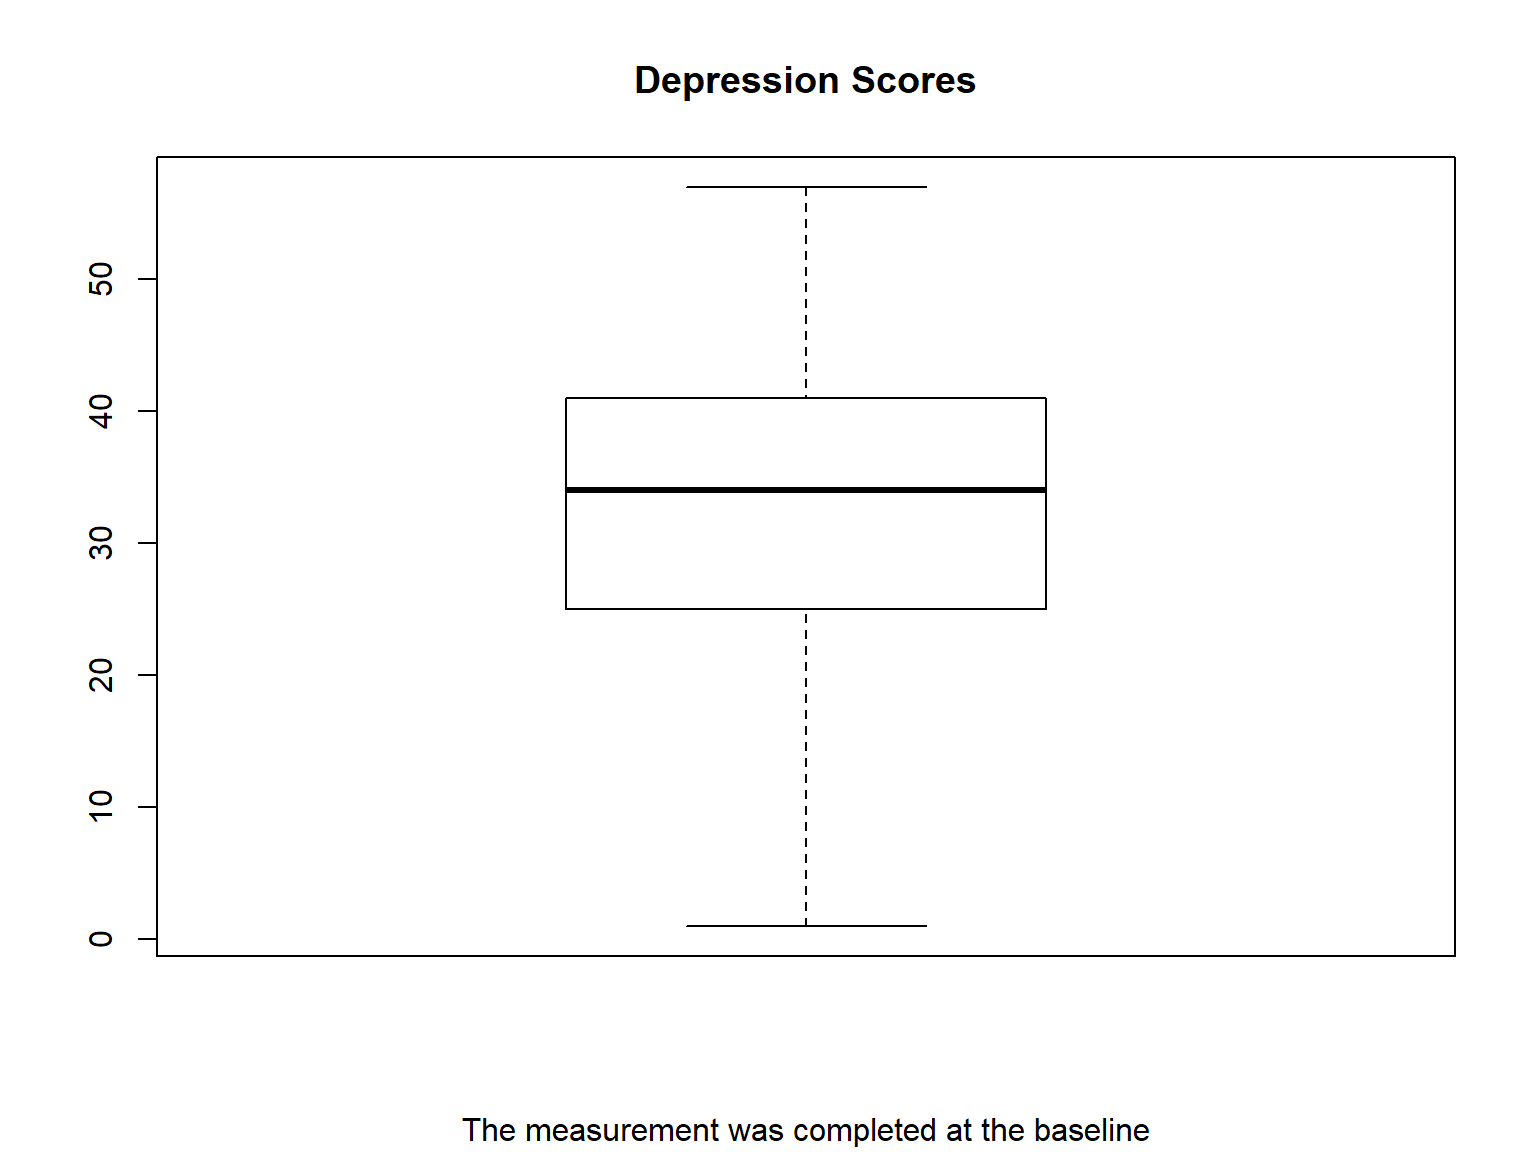
\includegraphics{rbook_files/figure-latex/boxplot1a-1} 

}

\caption{A boxplot example}\label{fig:boxplot1a}
\end{figure}

What \textbf{R} draws is shown in the figure, the most basic boxplot possible. When we look at this plot, this is how we should interpret it: the thick line in the middle of the box is the median; the box itself spans the range from the 25th percentile to the 75th percentile; and the ``whiskers'' cover the full range from the minimum value to the maximum value. This is summarised in the annotated plot in Figure \ref{fig:boxplot1b}.

\begin{figure}

{\centering 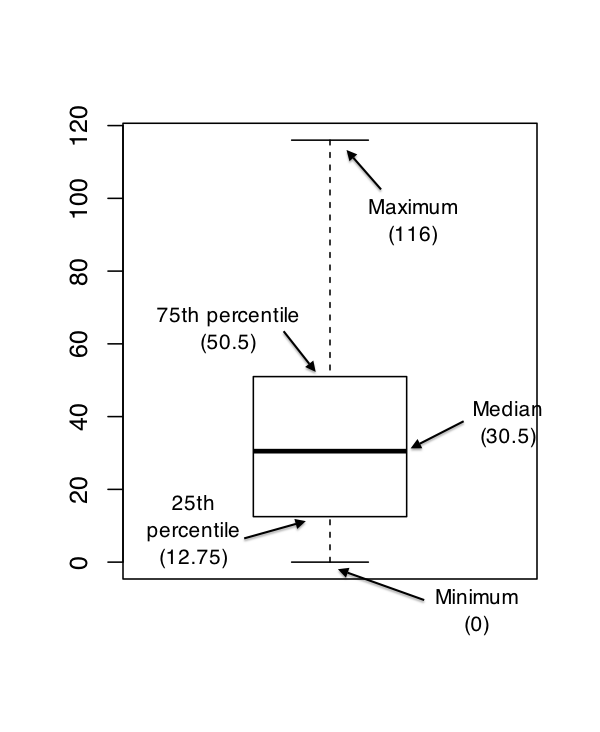
\includegraphics[width=8.33in]{figure/boxplot1_annotated} 

}

\caption{An annotated boxplot}\label{fig:boxplot1b}
\end{figure}

We can also draw multiple boxplots by a grouping variable. The way to do this using the \texttt{boxplot()} function is to input a \texttt{formula} rather than a variable as the input. Let's create a boxplot separated by sex.

\begin{Shaded}
\begin{Highlighting}[]
\KeywordTok{boxplot}\NormalTok{(}\DataTypeTok{formula =}\NormalTok{ depression1 }\OperatorTok{~}\StringTok{ }\NormalTok{sex,}
        \DataTypeTok{data =}\NormalTok{ medical,}
        \DataTypeTok{main =} \StringTok{"Depression Scores by Sex"}\NormalTok{,}
        \DataTypeTok{ylab =} \StringTok{"Depression at the baseline"}\NormalTok{,}
        \DataTypeTok{names =} \KeywordTok{c}\NormalTok{(}\StringTok{"Female"}\NormalTok{, }\StringTok{"Male"}\NormalTok{))}
\end{Highlighting}
\end{Shaded}

\begin{figure}

{\centering 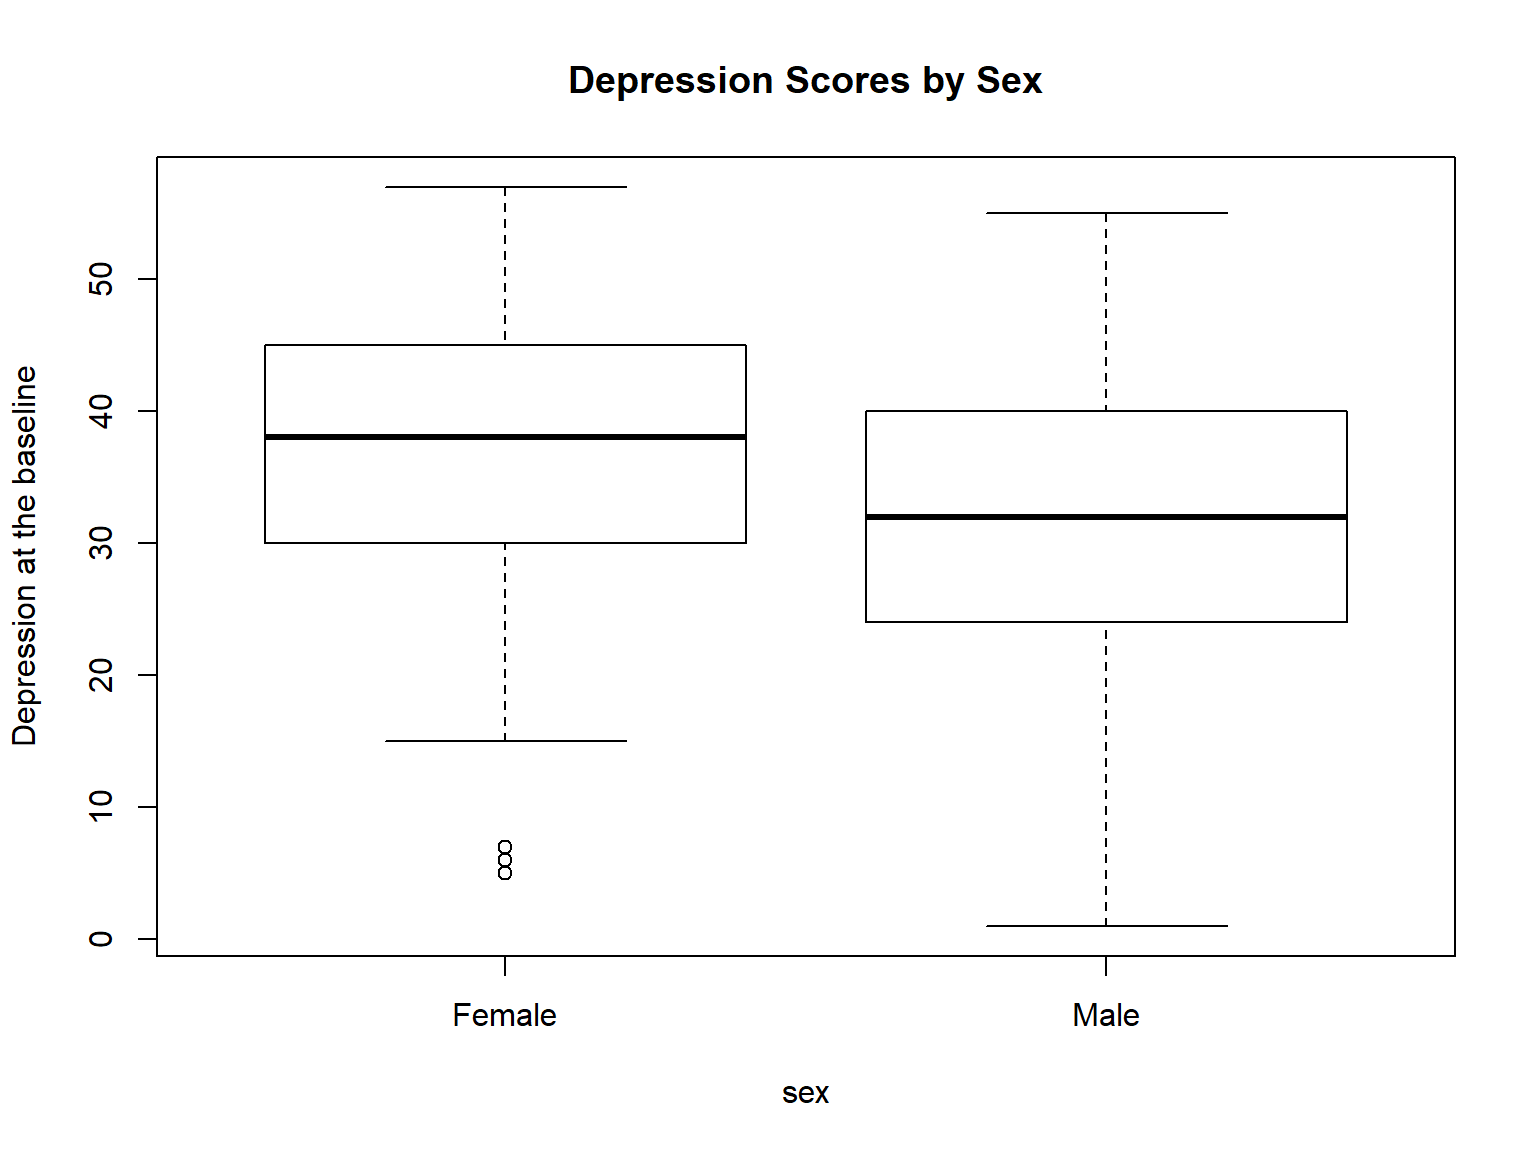
\includegraphics{rbook_files/figure-latex/boxplot2-1} 

}

\caption{A boxplot by a grouping variable}\label{fig:boxplot2}
\end{figure}

\hypertarget{histograms}{%
\subsection{Histograms}\label{histograms}}

\begin{Shaded}
\begin{Highlighting}[]
\KeywordTok{hist}\NormalTok{(medical}\OperatorTok{$}\NormalTok{depression1, }
     \DataTypeTok{main =} \StringTok{"Depression Scores at the Baseline"}\NormalTok{, }
     \DataTypeTok{xlab =} \StringTok{"Depression"}\NormalTok{)}
\end{Highlighting}
\end{Shaded}

\begin{figure}

{\centering 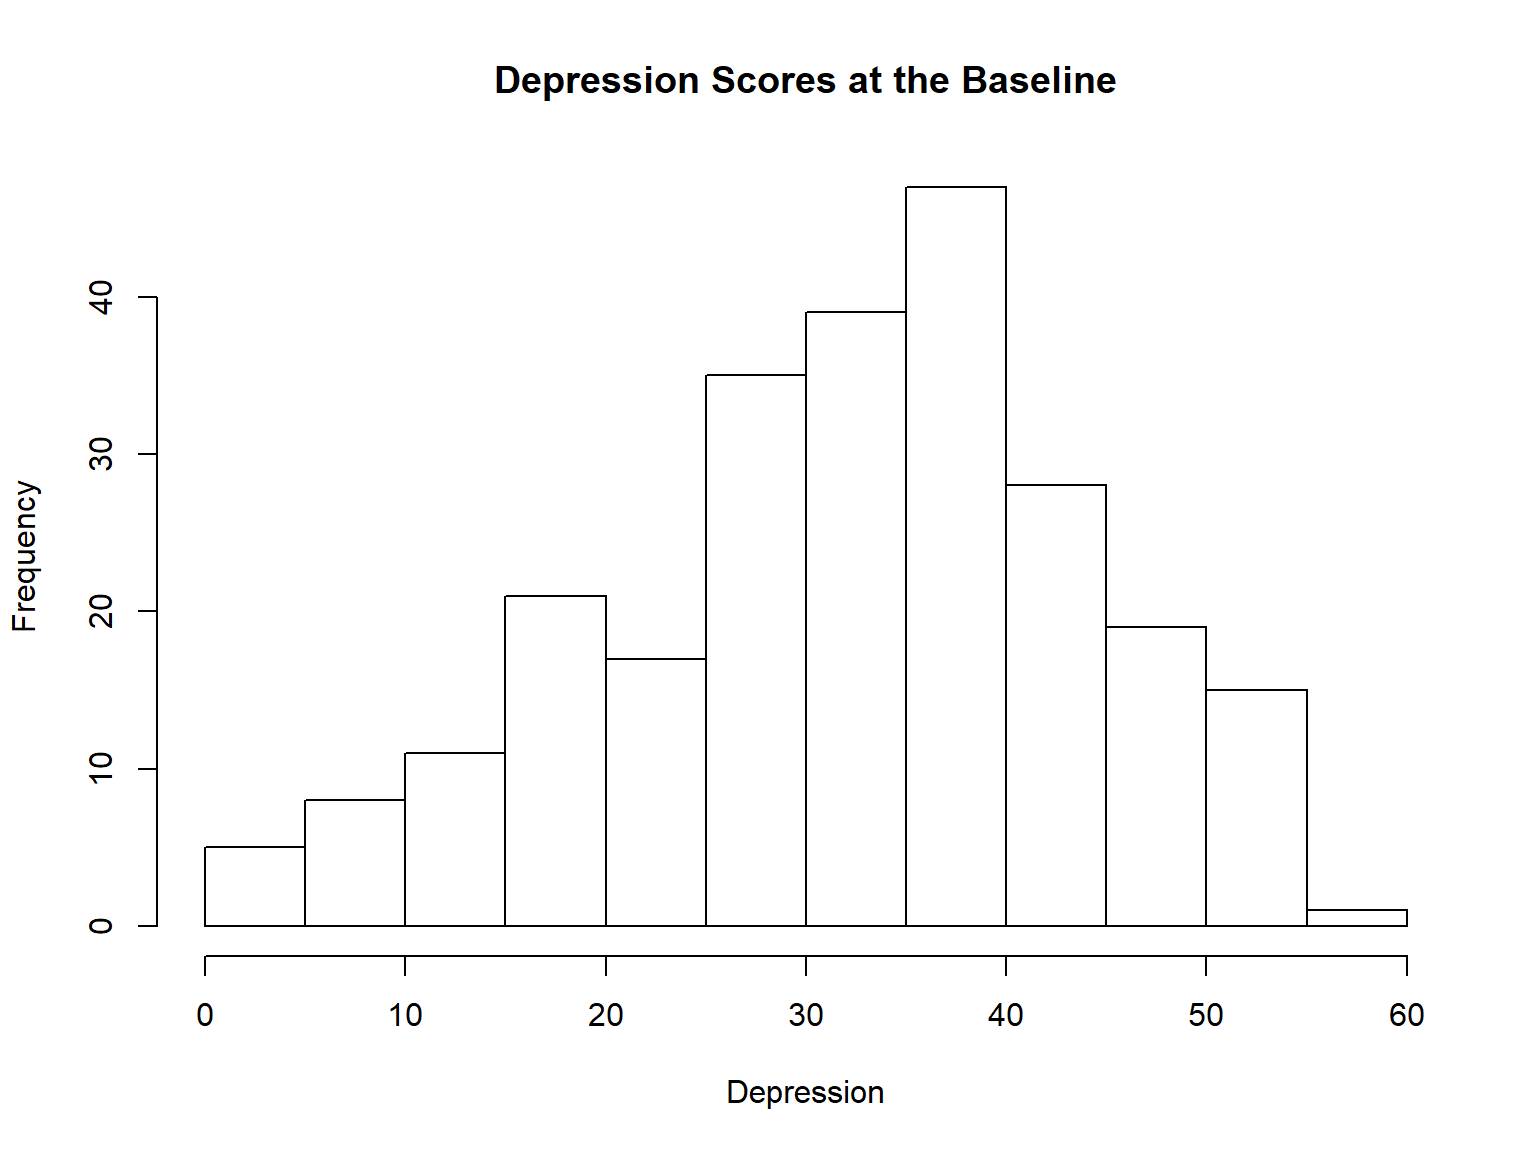
\includegraphics{rbook_files/figure-latex/histogram1-1} 

}

\caption{A histogram example}\label{fig:histogram1}
\end{figure}

Let's see the same histogram with additional changes on the font style and colors:

\begin{Shaded}
\begin{Highlighting}[]
\KeywordTok{hist}\NormalTok{(medical}\OperatorTok{$}\NormalTok{depression1, }
     \DataTypeTok{main =} \StringTok{"Depression Scores at the Baseline"}\NormalTok{, }
     \DataTypeTok{xlab =} \StringTok{"Depression"}\NormalTok{,}
     \DataTypeTok{font.main =} \DecValTok{1}\NormalTok{,}
     \DataTypeTok{cex.main =} \DecValTok{1}\NormalTok{,}
     \DataTypeTok{font.axis =} \DecValTok{2}\NormalTok{,}
     \DataTypeTok{col.lab =} \StringTok{"gray50"}\NormalTok{)}
\end{Highlighting}
\end{Shaded}

\begin{figure}

{\centering 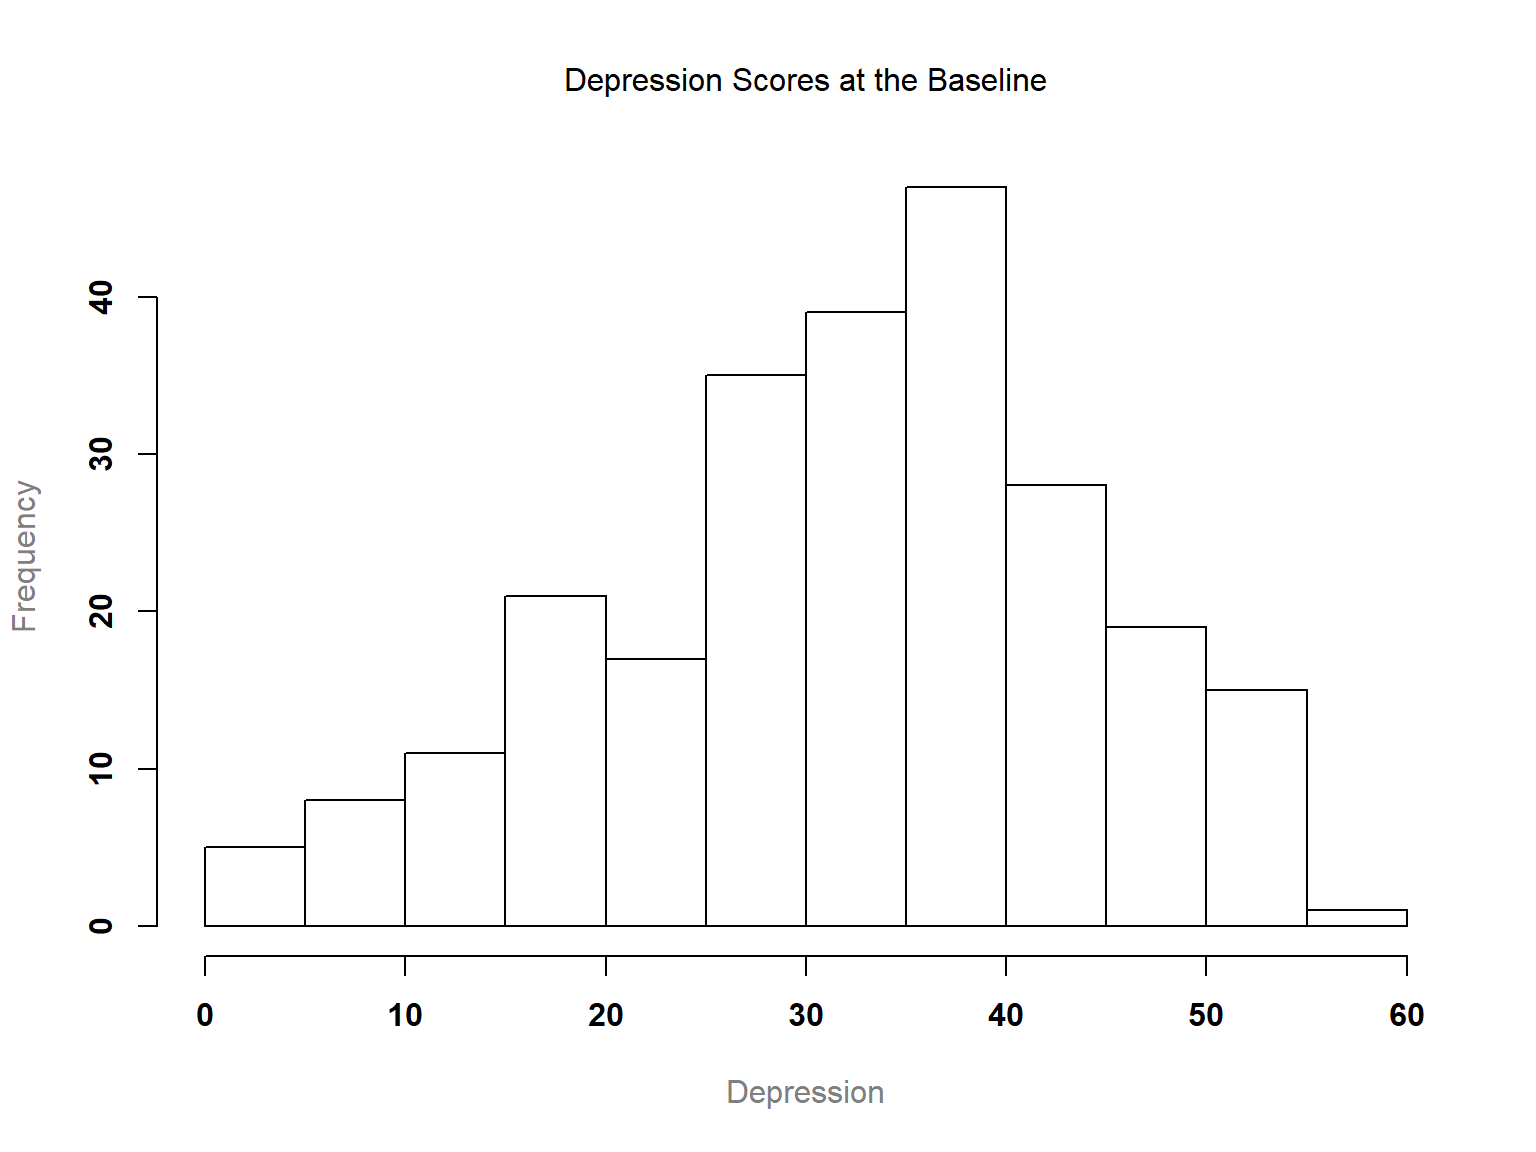
\includegraphics{rbook_files/figure-latex/histogram2-1} 

}

\caption{A histogram example (Edited)}\label{fig:histogram2}
\end{figure}

\hypertarget{bar-graphs}{%
\subsection{Bar Graphs}\label{bar-graphs}}

Bar plots are essentially plots for categorical variables (e.g., sex, race, etc.). Before we create a bar plot, we need to make sure that our categorical variables are ``factors'' -- i.e., labels. Otherwise, \textbf{R} attempts to treat such variables as quantative and thus fails to return a plot.

\begin{Shaded}
\begin{Highlighting}[]
\CommentTok{# Let's save race as a factor}
\NormalTok{medical}\OperatorTok{$}\NormalTok{race <-}\StringTok{ }\KeywordTok{as.factor}\NormalTok{(medical}\OperatorTok{$}\NormalTok{race)}

\CommentTok{# Create a bar graph for race}
\KeywordTok{plot}\NormalTok{(medical}\OperatorTok{$}\NormalTok{race, }
     \DataTypeTok{main =} \StringTok{"Race Groups in the medical Dataset"}\NormalTok{,}
     \DataTypeTok{xlab =} \StringTok{"Race"}\NormalTok{,}
     \DataTypeTok{ylab =} \StringTok{"Count"}\NormalTok{)}
\end{Highlighting}
\end{Shaded}

\begin{figure}

{\centering 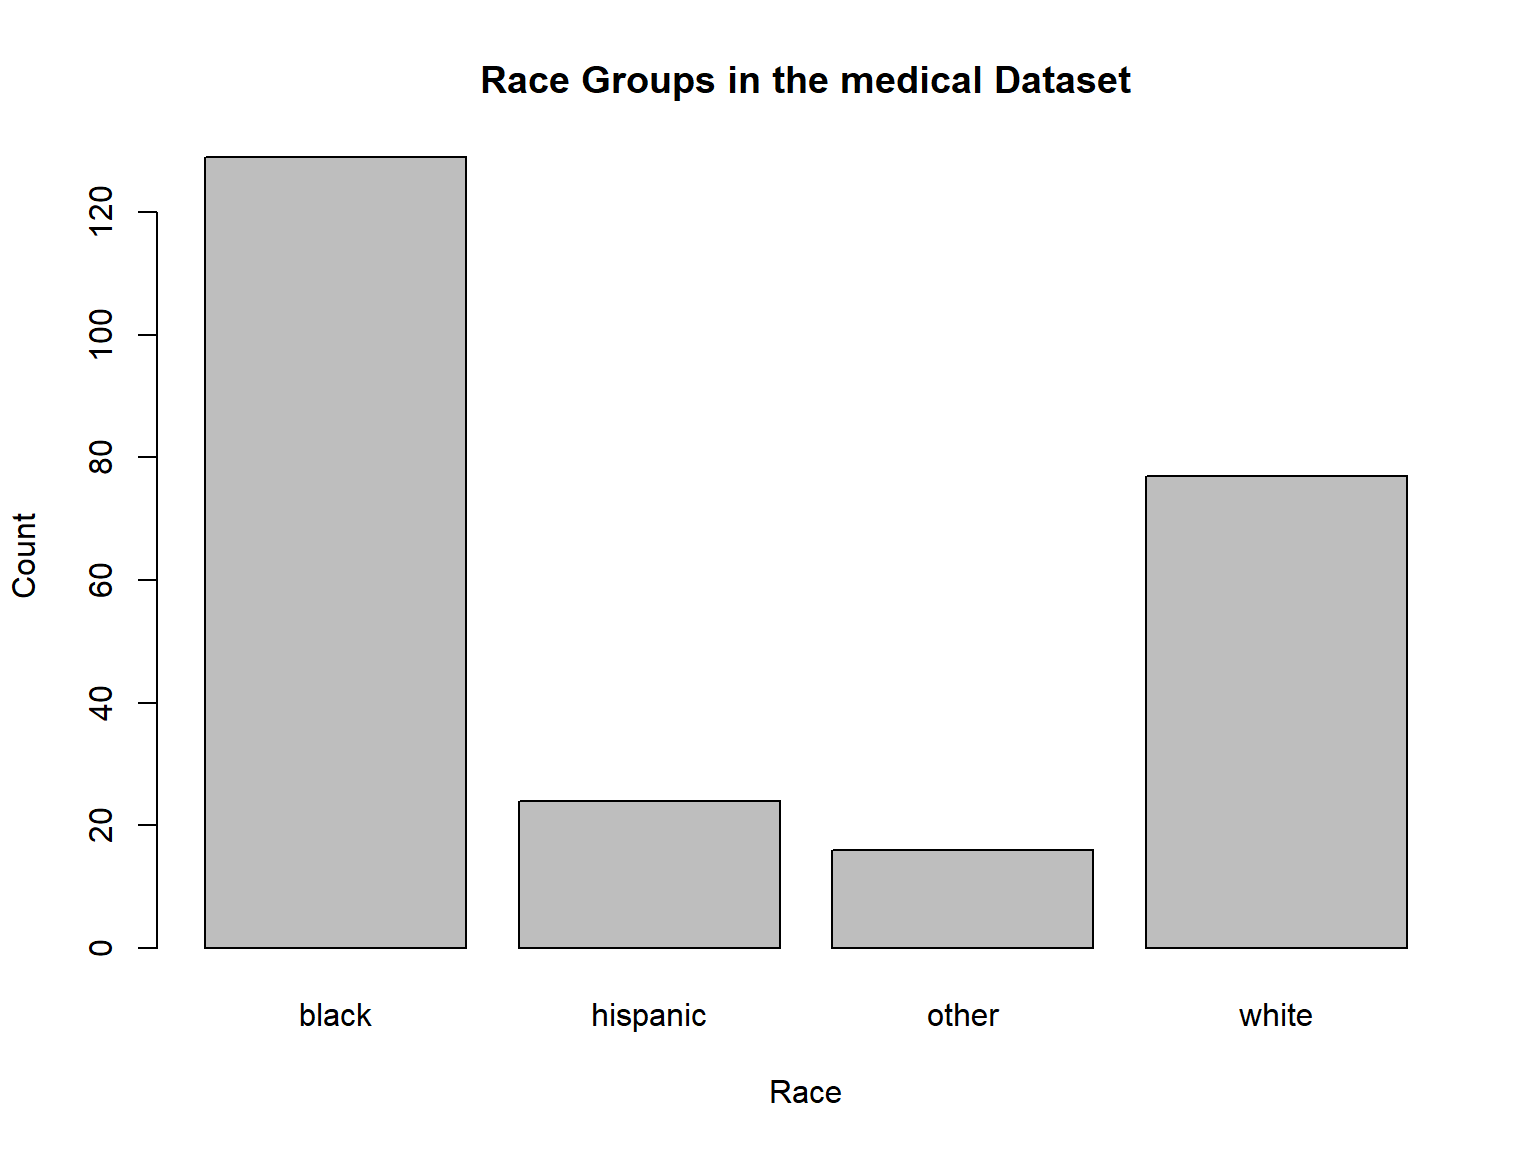
\includegraphics{rbook_files/figure-latex/bar-1} 

}

\caption{A bar graph example}\label{fig:bar}
\end{figure}

\hypertarget{scatterplots}{%
\subsection{Scatterplots}\label{scatterplots}}

\begin{Shaded}
\begin{Highlighting}[]
\KeywordTok{plot}\NormalTok{(medical}\OperatorTok{$}\NormalTok{depression1, medical}\OperatorTok{$}\NormalTok{depression2,}
     \DataTypeTok{xlab =} \StringTok{"Depression at the baseline"}\NormalTok{,}
     \DataTypeTok{ylab =} \StringTok{"Depression after 6 months"}\NormalTok{,}
     \DataTypeTok{main =} \StringTok{"Scatterplot of Depression Scores"}\NormalTok{)}
\end{Highlighting}
\end{Shaded}

\begin{figure}

{\centering 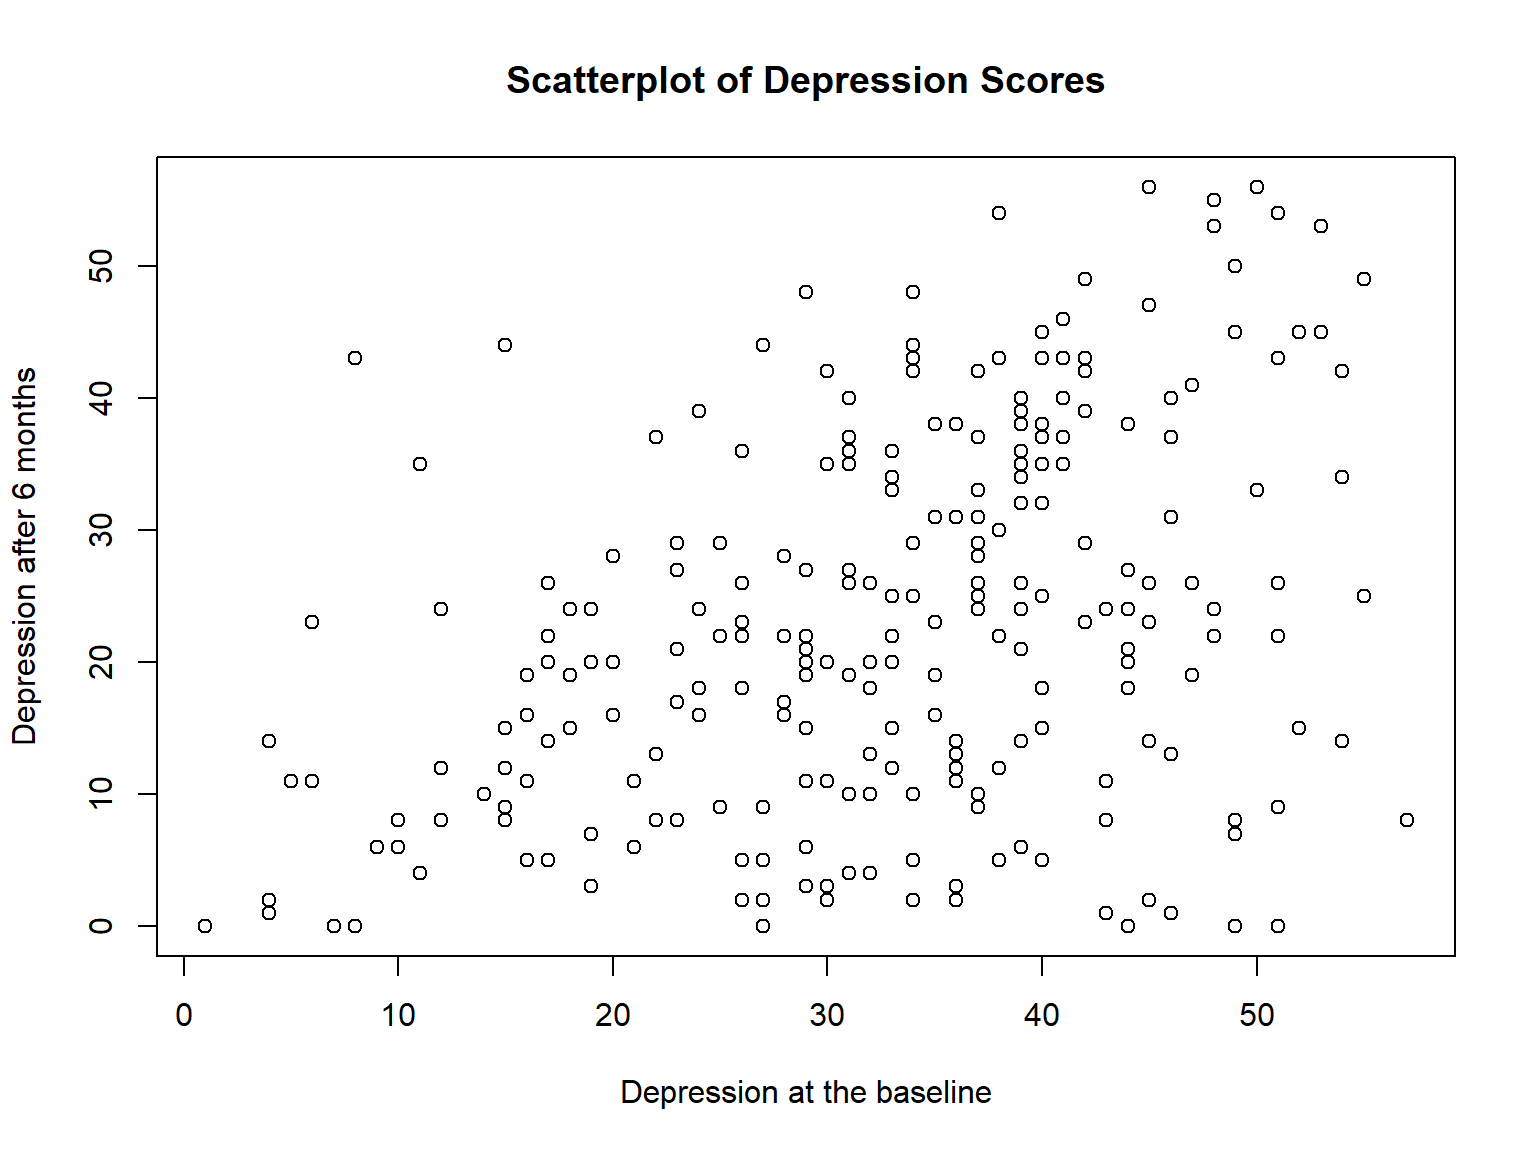
\includegraphics{rbook_files/figure-latex/scatter1-1} 

}

\caption{A scatterplot example}\label{fig:scatter1}
\end{figure}

We can customise the appearance of the actual plot. To start with, let's look at the single most important options that the \texttt{plot()} function provides for us to use, which is the \texttt{type} argument. The type argument specifies the visual style of the plot. The possible values for this are:

\begin{itemize}
\tightlist
\item
  \texttt{type\ =\ "p"}. Draw the \textbf{p}oints only
\item
  \texttt{type\ =\ "l"}. Draw a \textbf{l}ine through the points
\item
  \texttt{type\ =\ "o"}. Draw the line \textbf{o}ver the top of the points
\item
  \texttt{type\ =\ "b"}. Draw \textbf{b}oth points and lines, but don't overplot
\item
  \texttt{type\ =\ "h"}. Draw ``\textbf{h}istogram-like'' vertical bars
\item
  \texttt{type\ =\ "s"}. Draw a \textbf{s}taircase, going horizontally then vertically
\item
  \texttt{type\ =\ "S"}. Draw a \textbf{S}taircase, going vertically then horizontally
\item
  \texttt{type\ =\ "c"}. Draw only the \textbf{c}onnecting lines from the ``b'' version
\item
  \texttt{type\ =\ "n"}. Draw nothing
\end{itemize}

The simplest way to illustrate what each of these really looks like is just to draw them. Figure \ref{fig:simpleplots} shows a scatterplot using six different \texttt{types} of plot. As you can see, by altering the type argument we can get a qualitatively different appearance to our plot.

\begin{figure}

{\centering 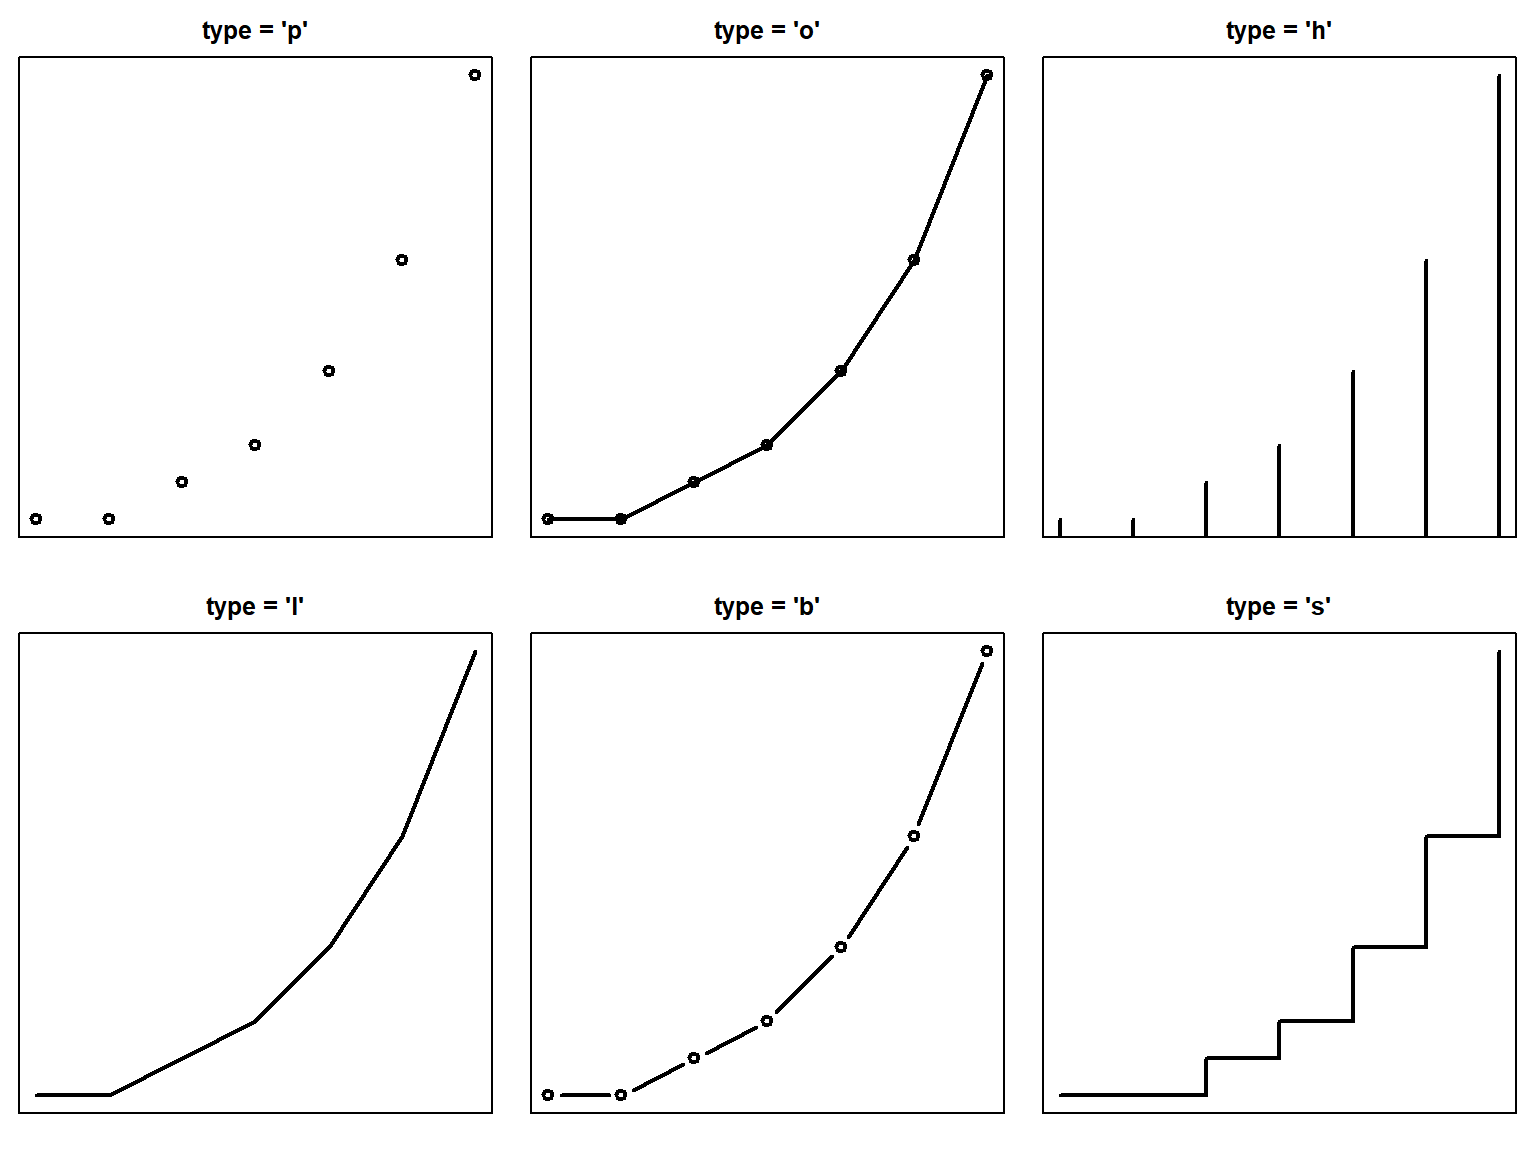
\includegraphics{rbook_files/figure-latex/simpleplots-1} 

}

\caption{Changing the `type` of the plot.}\label{fig:simpleplots}
\end{figure}

\hypertarget{scatterplots-boxplots}{%
\subsection{Scatterplots + Boxplots}\label{scatterplots-boxplots}}

The \texttt{scatterplot} function from the \texttt{car} package \citep{R-car} gives a nice plot that includes boxplots for individual variables and a scatterplot of the two variables together.

\begin{Shaded}
\begin{Highlighting}[]
\CommentTok{# Install and activate the car package}
\KeywordTok{install.packages}\NormalTok{(}\StringTok{"car"}\NormalTok{)}
\KeywordTok{library}\NormalTok{(}\StringTok{"car"}\NormalTok{)}

\KeywordTok{scatterplot}\NormalTok{(depression1 }\OperatorTok{~}\StringTok{ }\NormalTok{depression2, }
            \DataTypeTok{data =}\NormalTok{ medical, }
            \DataTypeTok{smooth =} \OtherTok{FALSE}\NormalTok{)}
\end{Highlighting}
\end{Shaded}

\begin{figure}

{\centering 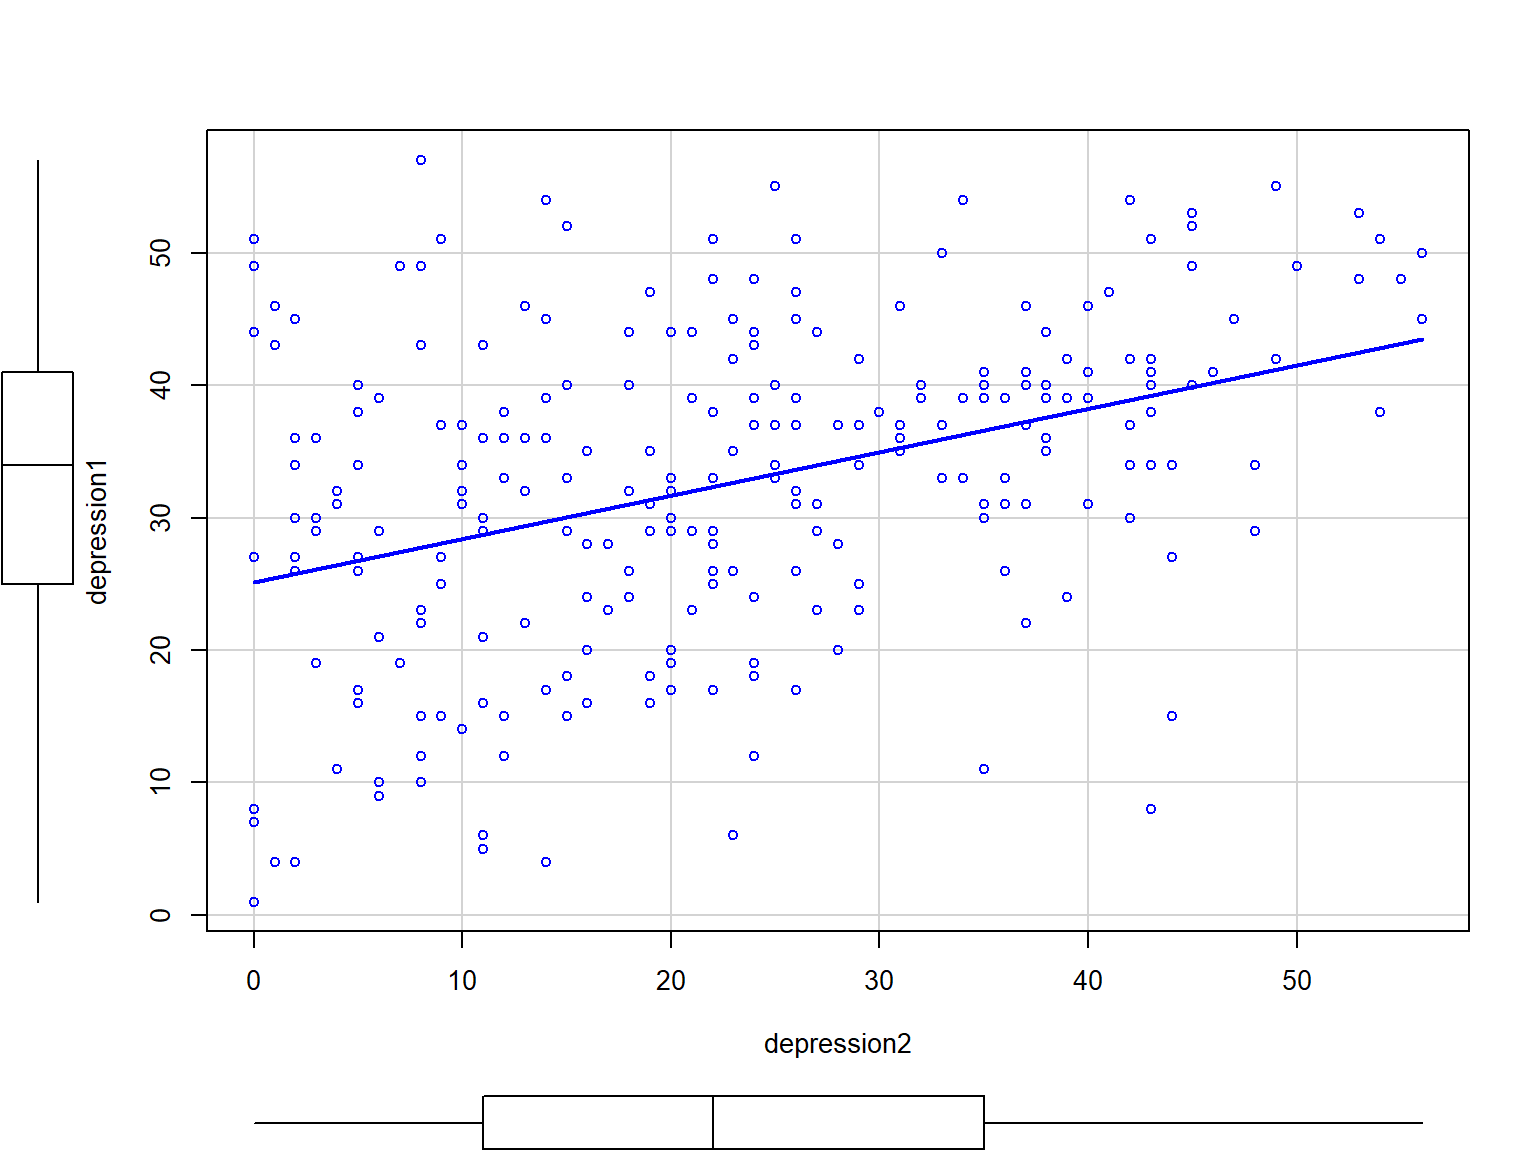
\includegraphics{rbook_files/figure-latex/scatter2-1} 

}

\caption{A scatterplot along with boxplots}\label{fig:scatter2}
\end{figure}

\hypertarget{scatterplot-matrix}{%
\subsection{Scatterplot Matrix}\label{scatterplot-matrix}}

Often we find yourself wanting to look at the relationships between several variables at once. One useful tool for doing so is to produce a ``scatterplot matrix'', analogous to the correlation matrix. We can create a scatterplot matrix using the \texttt{pairs} function in base \textbf{R}. Let's take a look at the following variables: depression1, mental1, and physical1.

\begin{Shaded}
\begin{Highlighting}[]
\KeywordTok{pairs}\NormalTok{(}\DataTypeTok{formula =} \OperatorTok{~}\StringTok{ }\NormalTok{depression1 }\OperatorTok{+}\StringTok{ }\NormalTok{mental1 }\OperatorTok{+}\StringTok{ }\NormalTok{physical1,}
      \DataTypeTok{data =}\NormalTok{ medical,}
      \DataTypeTok{main =} \StringTok{"Scatterplot Matrix with Three Scores"}\NormalTok{)}
\end{Highlighting}
\end{Shaded}

\begin{figure}

{\centering 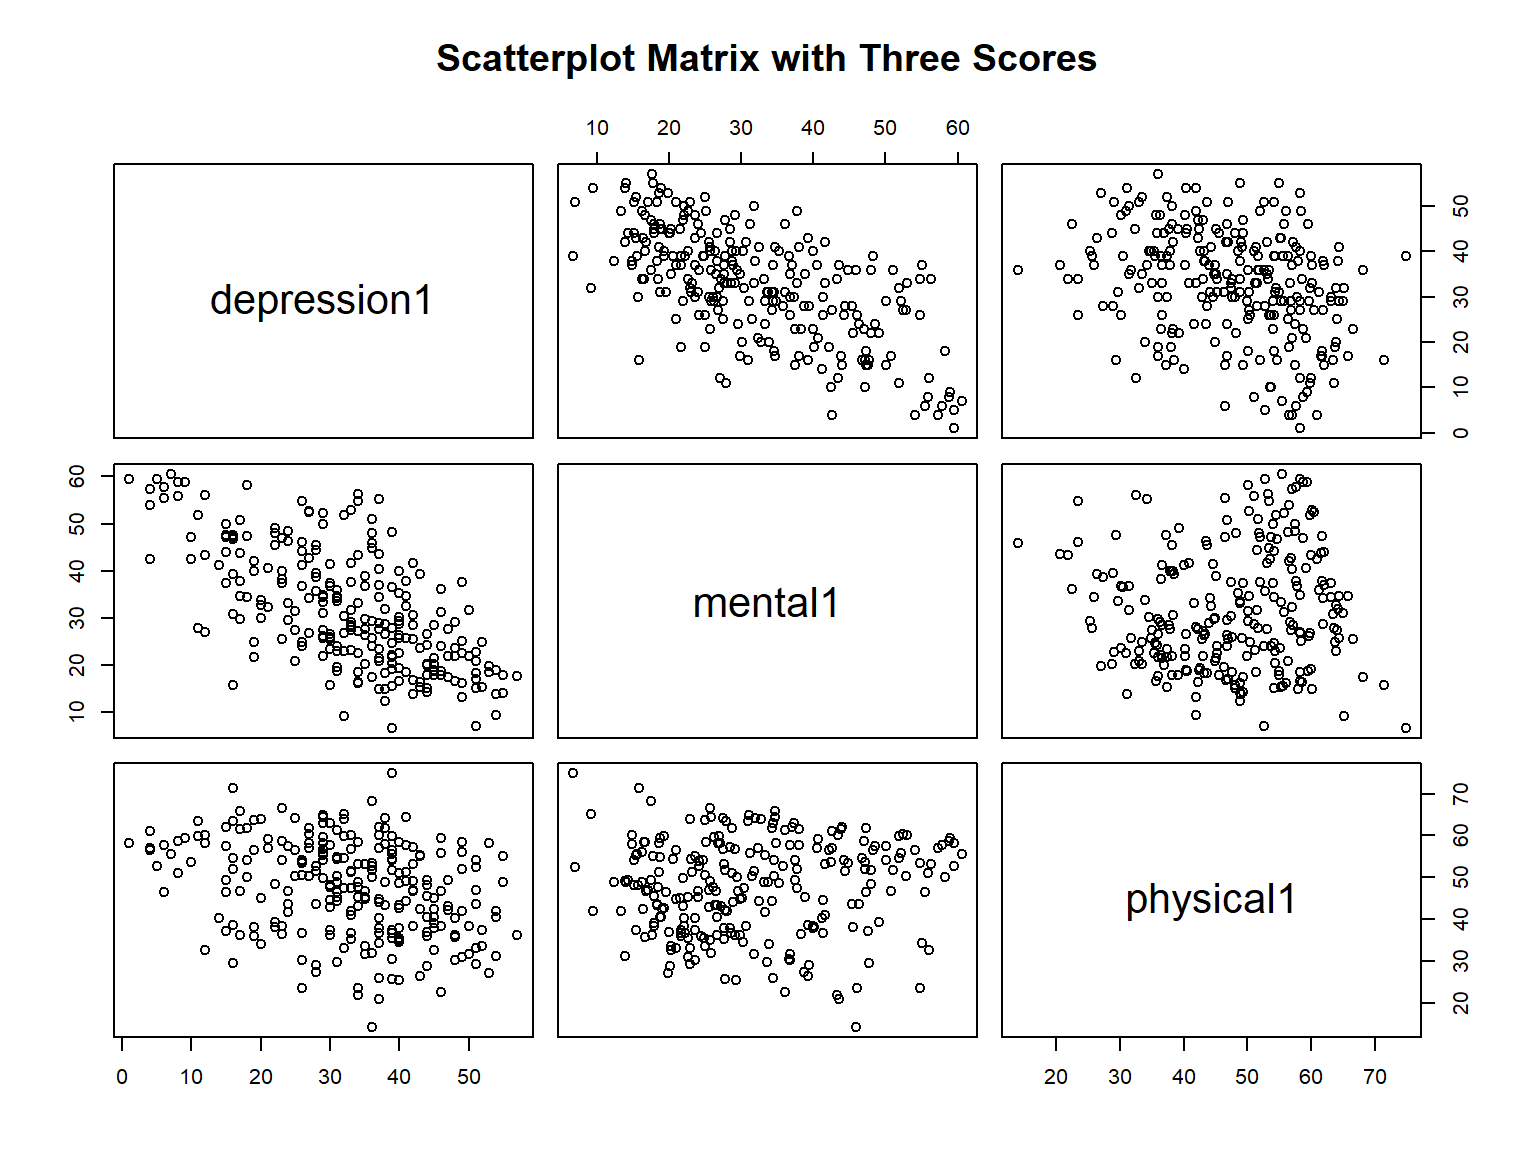
\includegraphics{rbook_files/figure-latex/scatter3-1} 

}

\caption{A scatterplot matrix from the `pairs()` function}\label{fig:scatter3}
\end{figure}

\hypertarget{saving-base-r-figures}{%
\subsection{\texorpdfstring{Saving Base \textbf{R} Figures}{Saving Base R Figures}}\label{saving-base-r-figures}}

We can save figures generated by base \textbf{R} functions in several ways:

\begin{itemize}
\tightlist
\item
  \texttt{jpeg("filename.jpg")}
\item
  \texttt{png("filename.jpng")}
\item
  \texttt{pdf("filename.pdf")}
\item
  \texttt{tiff("filename.tif")}
\end{itemize}

For example, to save our plot using .jpg format, we would do:

\begin{Shaded}
\begin{Highlighting}[]
\KeywordTok{jpeg}\NormalTok{(}\StringTok{"myplot.jpg"}\NormalTok{, }\DataTypeTok{width =} \DecValTok{8}\NormalTok{, }\DataTypeTok{height =} \DecValTok{4}\NormalTok{, }\DataTypeTok{units =} \StringTok{"in"}\NormalTok{, }\DataTypeTok{res =} \DecValTok{300}\NormalTok{)}
\KeywordTok{plot}\NormalTok{(medical}\OperatorTok{$}\NormalTok{depression1, medical}\OperatorTok{$}\NormalTok{depression2)}
\KeywordTok{dev.off}\NormalTok{()}
\end{Highlighting}
\end{Shaded}

where \texttt{width} and \texttt{height} are dimensions in inches (\texttt{units\ =\ "in"}) and resolution is 300 dpi.

\hypertarget{your-turn-6}{%
\subsection{Your Turn}\label{your-turn-6}}

Here you will create two plots:

\begin{enumerate}
\def\labelenumi{\arabic{enumi}.}
\item
  A boxplot of \texttt{mental1} (i.e., mental test scores at the baseline) by \texttt{substance} (i.e., type of substance being used). Do you see any differences between the mental test scores of the three substance groups?
\item
  A scatterplot of \texttt{depression1} against \texttt{mental1}. You need to see the depression scores on the x-axis and the mental test scores on the y-axis. What type of relationship do you see between the two variables (e.g., negative, positive, or no relationship)?
\end{enumerate}

\hypertarget{ggplot2-graphics}{%
\section{\texorpdfstring{\texttt{ggplot2} Graphics}{ggplot2 Graphics}}\label{ggplot2-graphics}}

\hypertarget{what-is-ggplot2}{%
\subsection{\texorpdfstring{What is \texttt{ggplot2}?}{What is ggplot2?}}\label{what-is-ggplot2}}

\begin{itemize}
\tightlist
\item
  A comprehensive data visualization package in \textbf{R}
\item
  Popular method for creating explanatory graphics
\item
  Simpler than base \textbf{R} graphics due its multi-layer approach
\item
  Many other supplementary packages using the \texttt{ggplot2} platform
\end{itemize}

\hypertarget{how-ggplot2-works}{%
\subsection{\texorpdfstring{How \texttt{ggplot2} works?}{How ggplot2 works?}}\label{how-ggplot2-works}}

The \texttt{ggplot2} package \citep{R-ggplot2} follows data visualization rules known as ``The Grammar of Graphics''. The grammar tells us that a statistical graphic is a \textbf{mapping} of data variables to \textbf{aesthetic} attributes of \textbf{geometric} objects.

Specifically, we can break a graphic into the following three essential components:

\begin{itemize}
\tightlist
\item
  \texttt{data}: the data set composed of variables that we map.
\item
  \texttt{geom}: the geometric object in question. This refers to the type of object we can observe in a plot. For example: points, lines, and bars.
\item
  \texttt{aes}: aesthetic attributes of the geometric object. For example, color, shape, and size. Each assigned aesthetic attribute can be mapped to a variable in our data set.
\end{itemize}

Figure \ref{fig:ggplotmap} shows these three components are laied out in a typical \texttt{ggplot2} function. As we can see, each part (e.g., \texttt{geom\_function}) is added to the plot using a plus sign. That is, each layer like that brings an additional functionality into the plot we are drawing.

\begin{figure}

{\centering 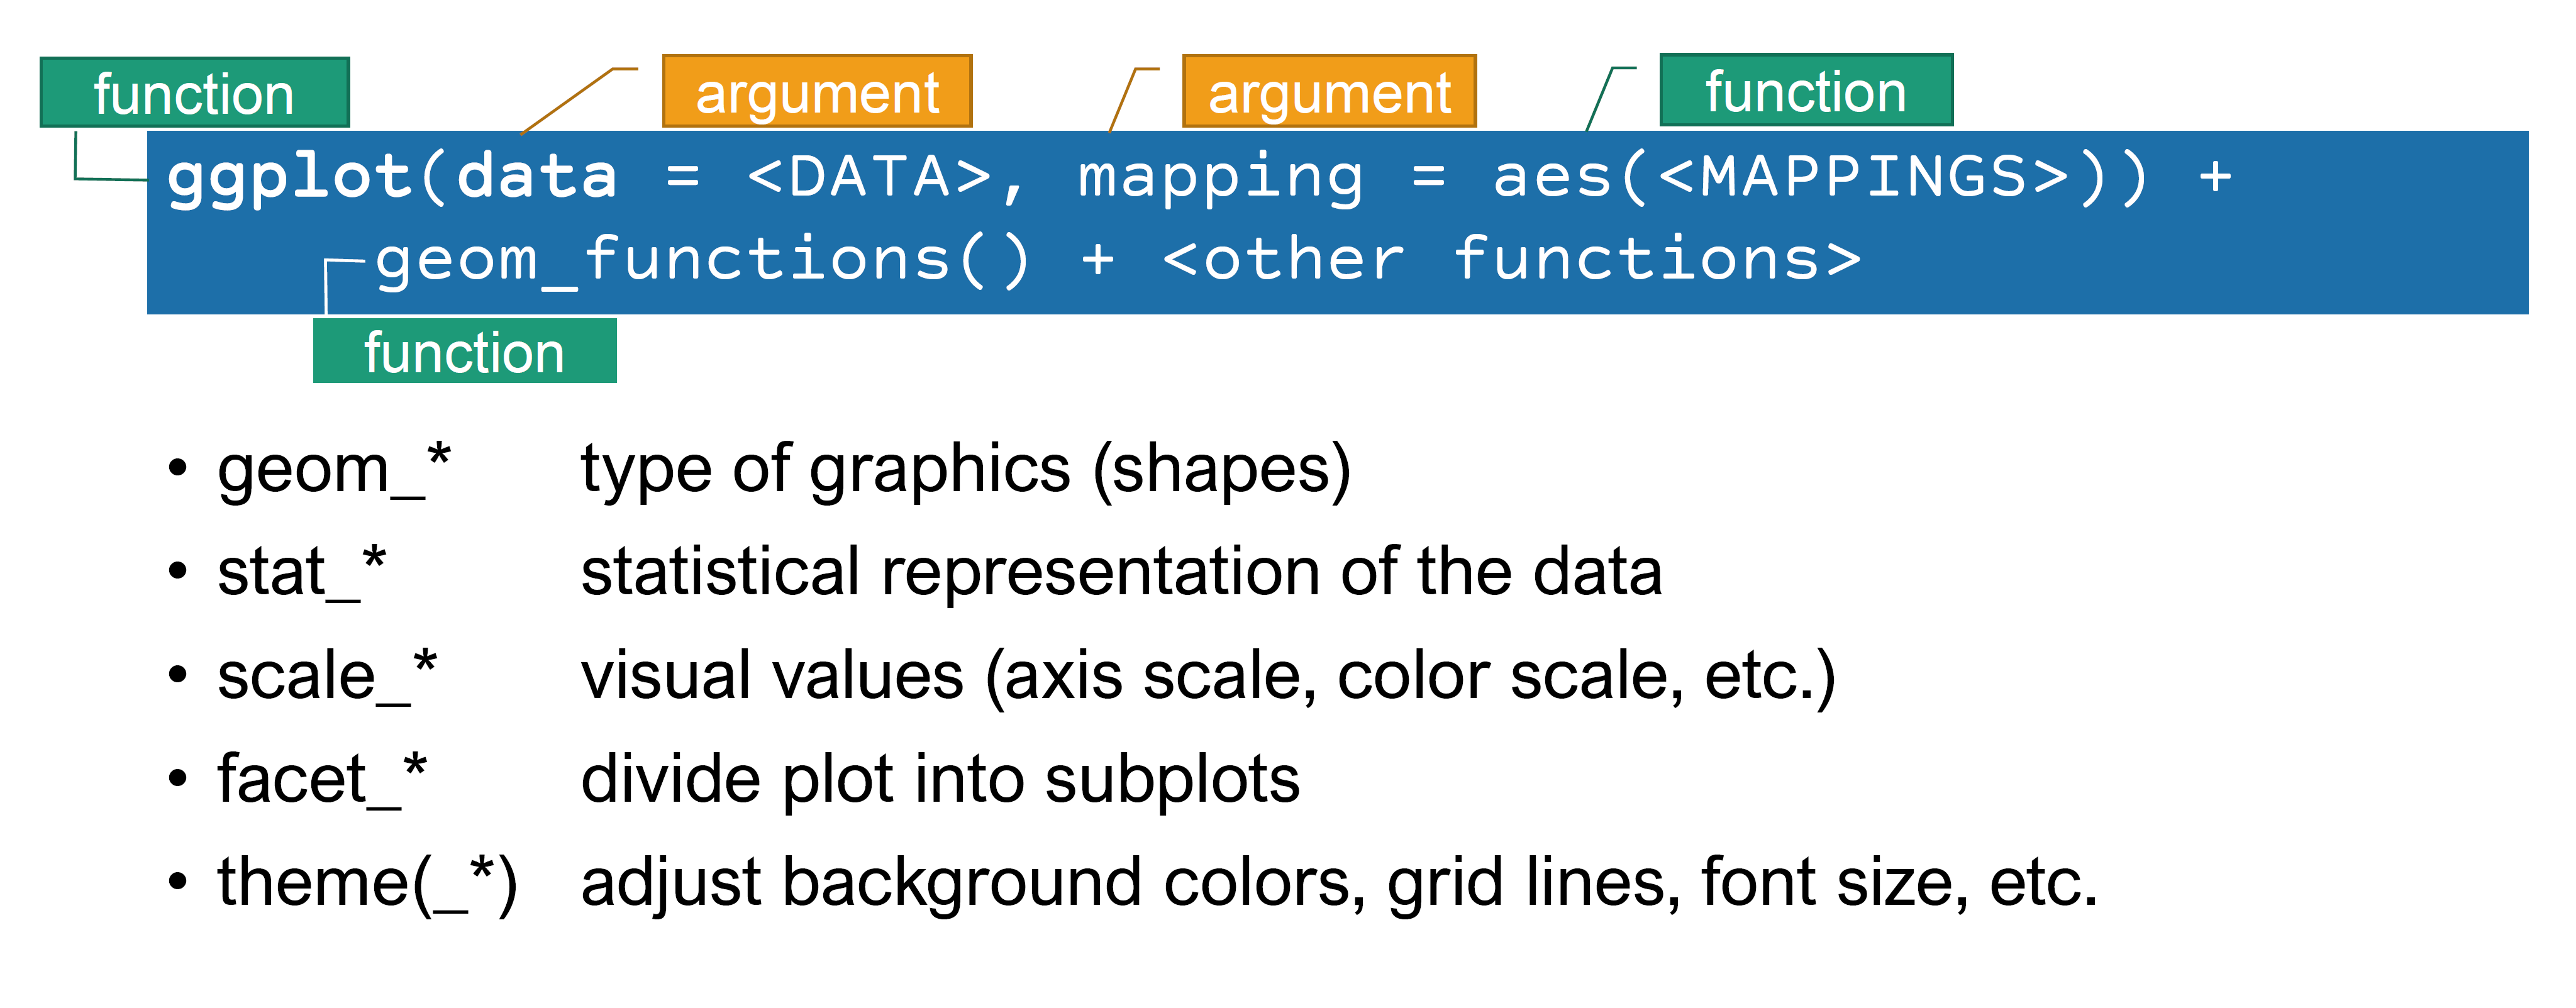
\includegraphics[width=0.65\linewidth]{figure/ggplot} 

}

\caption{How the elements of `ggplot2` work}\label{fig:ggplotmap}
\end{figure}

In order to keep things simple, we will only take a look at the following types of graphics in \texttt{ggplot2}:

\begin{itemize}
\tightlist
\item
  scatterplots
\item
  boxplots
\item
  histograms
\item
  bar plots
\end{itemize}

For more information on \texttt{ggplot2}, check out \url{http://ggplot2.tidyverse.org/}.

\hypertarget{scatterplots-1}{%
\subsection{Scatterplots}\label{scatterplots-1}}

\begin{Shaded}
\begin{Highlighting}[]
\CommentTok{# Activate the package first}
\KeywordTok{library}\NormalTok{(}\StringTok{"ggplot2"}\NormalTok{)}

\KeywordTok{ggplot}\NormalTok{(}\DataTypeTok{data =}\NormalTok{ medical, }
       \DataTypeTok{mapping =} \KeywordTok{aes}\NormalTok{(depression1, depression2)) }\OperatorTok{+}\StringTok{ }
\StringTok{  }\KeywordTok{geom_point}\NormalTok{(}\DataTypeTok{size =} \DecValTok{3}\NormalTok{) }\OperatorTok{+}
\StringTok{  }\KeywordTok{labs}\NormalTok{(}\DataTypeTok{x =} \StringTok{"Depression (Baseline)"}\NormalTok{, }
       \DataTypeTok{y =} \StringTok{"Depression (6 months)"}\NormalTok{) }\OperatorTok{+}
\StringTok{  }\KeywordTok{theme_bw}\NormalTok{() }\CommentTok{# for black & white theme}
\end{Highlighting}
\end{Shaded}

\begin{figure}

{\centering 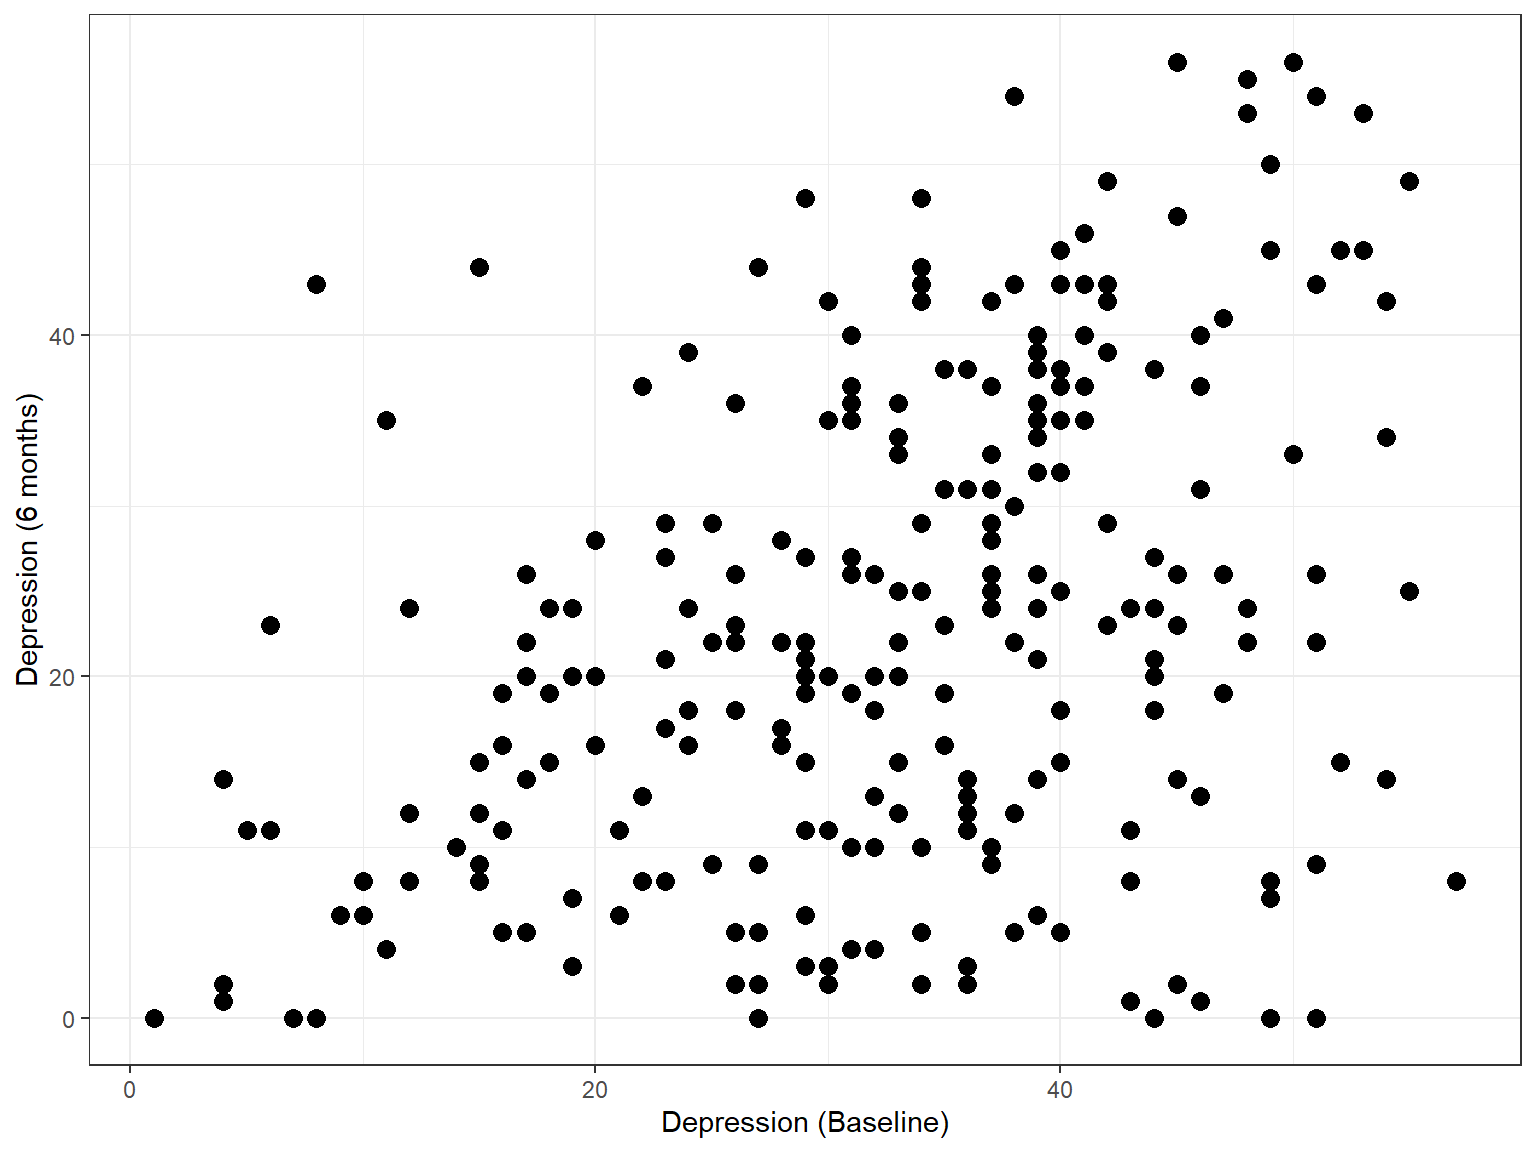
\includegraphics{rbook_files/figure-latex/ggscatter1-1} 

}

\caption{A scatterplot example with `ggplot2`}\label{fig:ggscatter1}
\end{figure}

\begin{Shaded}
\begin{Highlighting}[]
\KeywordTok{ggplot}\NormalTok{(}\DataTypeTok{data =}\NormalTok{ medical, }
       \DataTypeTok{mapping =} \KeywordTok{aes}\NormalTok{(depression1, depression2, }\DataTypeTok{colour =}\NormalTok{ sex)) }\OperatorTok{+}\StringTok{ }
\StringTok{  }\KeywordTok{geom_point}\NormalTok{(}\DataTypeTok{size =} \DecValTok{3}\NormalTok{) }\OperatorTok{+}
\StringTok{  }\KeywordTok{geom_smooth}\NormalTok{(}\DataTypeTok{method =}\NormalTok{ lm, }\DataTypeTok{color =} \StringTok{"red"}\NormalTok{, }\DataTypeTok{se =} \OtherTok{TRUE}\NormalTok{) }\OperatorTok{+}
\StringTok{  }\KeywordTok{labs}\NormalTok{(}\DataTypeTok{colour =} \StringTok{"Sex"}\NormalTok{, }
       \DataTypeTok{x =} \StringTok{"Depression (Baseline)"}\NormalTok{, }
       \DataTypeTok{y =} \StringTok{"Depression (6 months)"}\NormalTok{) }\OperatorTok{+}
\StringTok{  }\KeywordTok{theme_bw}\NormalTok{() }\CommentTok{# for black & white theme}
\end{Highlighting}
\end{Shaded}

\begin{figure}

{\centering 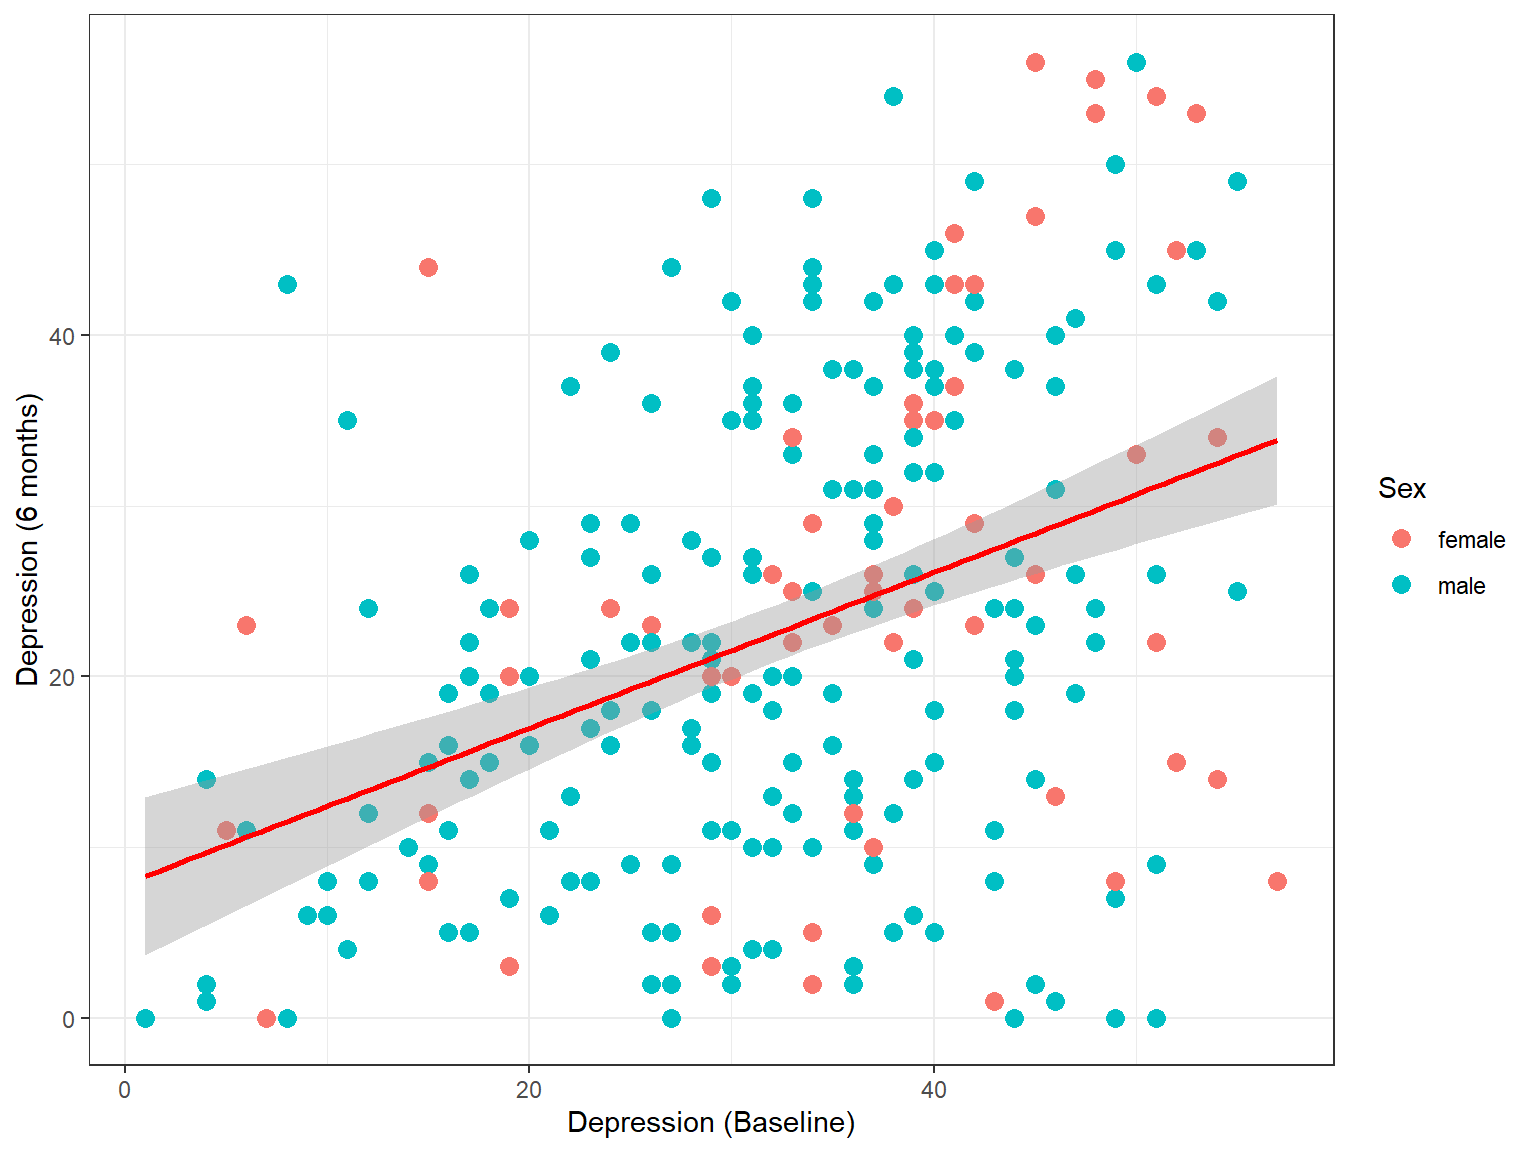
\includegraphics{rbook_files/figure-latex/ggscatter2-1} 

}

\caption{A scatterplot example with `ggplot2` (With regression line)}\label{fig:ggscatter2}
\end{figure}

\hypertarget{boxplots-1}{%
\subsection{Boxplots}\label{boxplots-1}}

\begin{Shaded}
\begin{Highlighting}[]
\KeywordTok{ggplot}\NormalTok{(}\DataTypeTok{data =}\NormalTok{ medical, }
       \DataTypeTok{mapping =} \KeywordTok{aes}\NormalTok{(}\DataTypeTok{x =}\NormalTok{ sex, }\DataTypeTok{y =}\NormalTok{ depression1, }\DataTypeTok{fill =}\NormalTok{ race)) }\OperatorTok{+}\StringTok{ }
\StringTok{  }\KeywordTok{labs}\NormalTok{(}\DataTypeTok{x =} \StringTok{"Sex"}\NormalTok{, }
       \DataTypeTok{y =} \StringTok{"Depression at the baseline"}\NormalTok{, }
       \DataTypeTok{fill =} \StringTok{"Race"}\NormalTok{) }\OperatorTok{+}\StringTok{ }
\StringTok{  }\KeywordTok{geom_boxplot}\NormalTok{() }\OperatorTok{+}
\StringTok{  }\KeywordTok{theme_bw}\NormalTok{()}
\end{Highlighting}
\end{Shaded}

\begin{figure}

{\centering 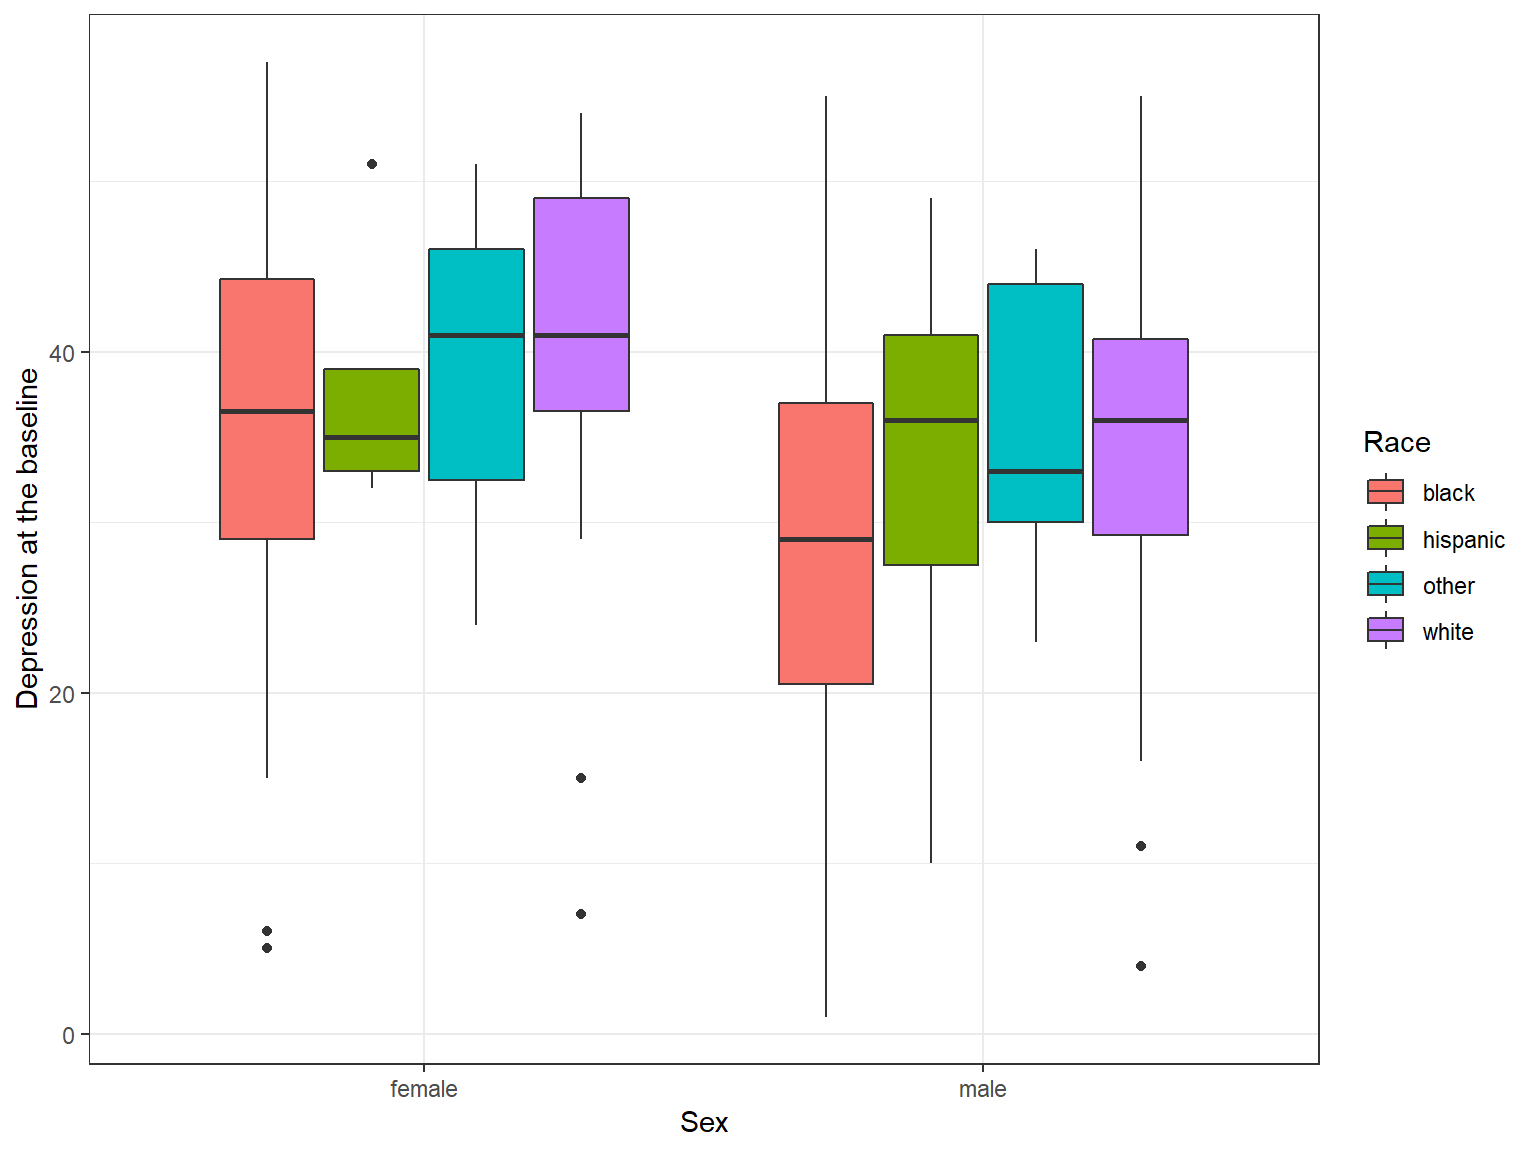
\includegraphics{rbook_files/figure-latex/ggboxplot-1} 

}

\caption{A boxplot example with `ggplot2`}\label{fig:ggboxplot}
\end{figure}

\hypertarget{histograms-1}{%
\subsection{Histograms}\label{histograms-1}}

\begin{Shaded}
\begin{Highlighting}[]
\KeywordTok{ggplot}\NormalTok{(}\DataTypeTok{data =}\NormalTok{ medical, }
       \DataTypeTok{mapping =} \KeywordTok{aes}\NormalTok{(}\DataTypeTok{x =}\NormalTok{ depression1)) }\OperatorTok{+}\StringTok{ }
\StringTok{  }\KeywordTok{labs}\NormalTok{(}\DataTypeTok{x =} \StringTok{"Depression at the baseline"}\NormalTok{,}
       \DataTypeTok{y =} \StringTok{"Frequency"}\NormalTok{,}
       \DataTypeTok{title =} \StringTok{"Depression Scores at the the Baseline"}\NormalTok{) }\OperatorTok{+}\StringTok{ }
\StringTok{  }\KeywordTok{geom_histogram}\NormalTok{(}\DataTypeTok{color =} \StringTok{"white"}\NormalTok{, }\CommentTok{# color of bar lines}
                 \DataTypeTok{fill =} \StringTok{"steelblue"}\NormalTok{, }\CommentTok{# filling color}
                 \DataTypeTok{bins =} \DecValTok{40}\NormalTok{) }\OperatorTok{+}\StringTok{ }\CommentTok{# number of bins}
\StringTok{  }\KeywordTok{theme_bw}\NormalTok{()}
\end{Highlighting}
\end{Shaded}

\begin{figure}

{\centering 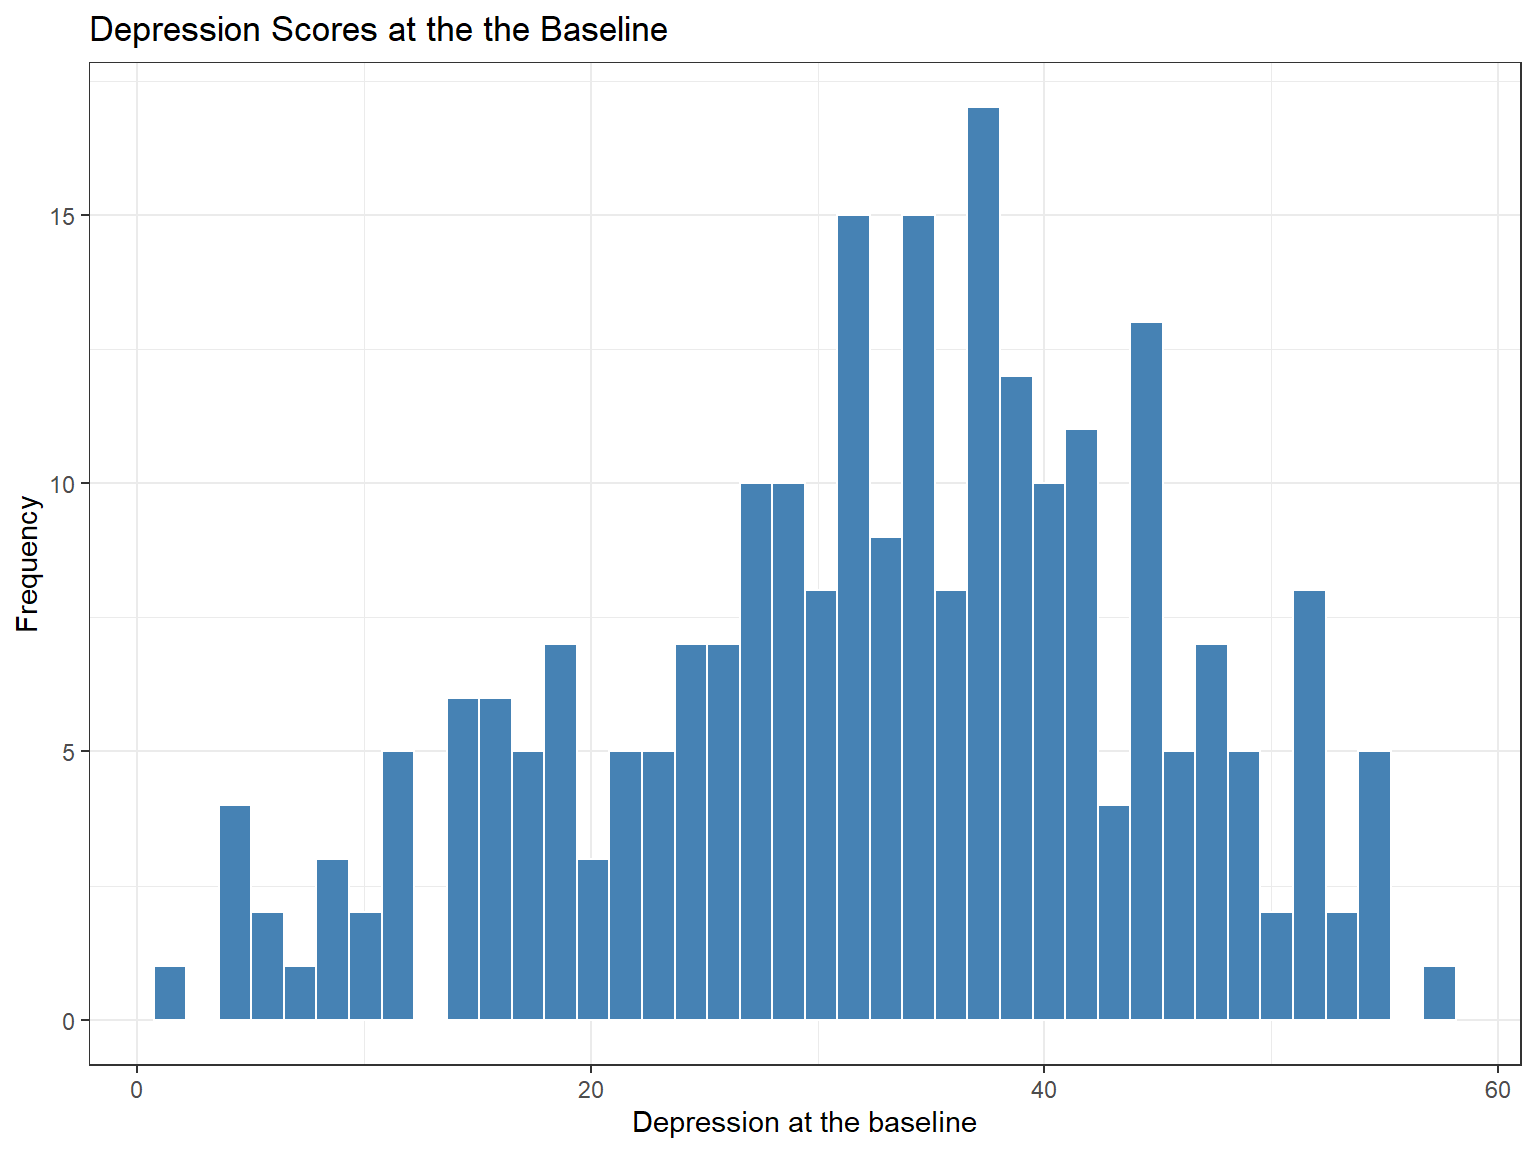
\includegraphics{rbook_files/figure-latex/gghistogram-1} 

}

\caption{A histogram example with `ggplot2`}\label{fig:gghistogram}
\end{figure}

\hypertarget{bar-plots}{%
\subsection{Bar Plots}\label{bar-plots}}

\begin{Shaded}
\begin{Highlighting}[]
\KeywordTok{ggplot}\NormalTok{(}\DataTypeTok{data =}\NormalTok{ medical, }
       \DataTypeTok{mapping =} \KeywordTok{aes}\NormalTok{(}\DataTypeTok{x =}\NormalTok{ race)) }\OperatorTok{+}\StringTok{ }
\StringTok{  }\KeywordTok{labs}\NormalTok{(}\DataTypeTok{x =} \StringTok{"Race"}\NormalTok{,}
       \DataTypeTok{y =} \StringTok{"Frequency"}\NormalTok{) }\OperatorTok{+}\StringTok{ }
\StringTok{  }\KeywordTok{geom_bar}\NormalTok{(}\DataTypeTok{color =} \StringTok{"white"}\NormalTok{,}
           \DataTypeTok{fill =} \StringTok{"orange"}\NormalTok{) }\OperatorTok{+}
\StringTok{  }\KeywordTok{theme_bw}\NormalTok{()}
\end{Highlighting}
\end{Shaded}

\begin{figure}

{\centering 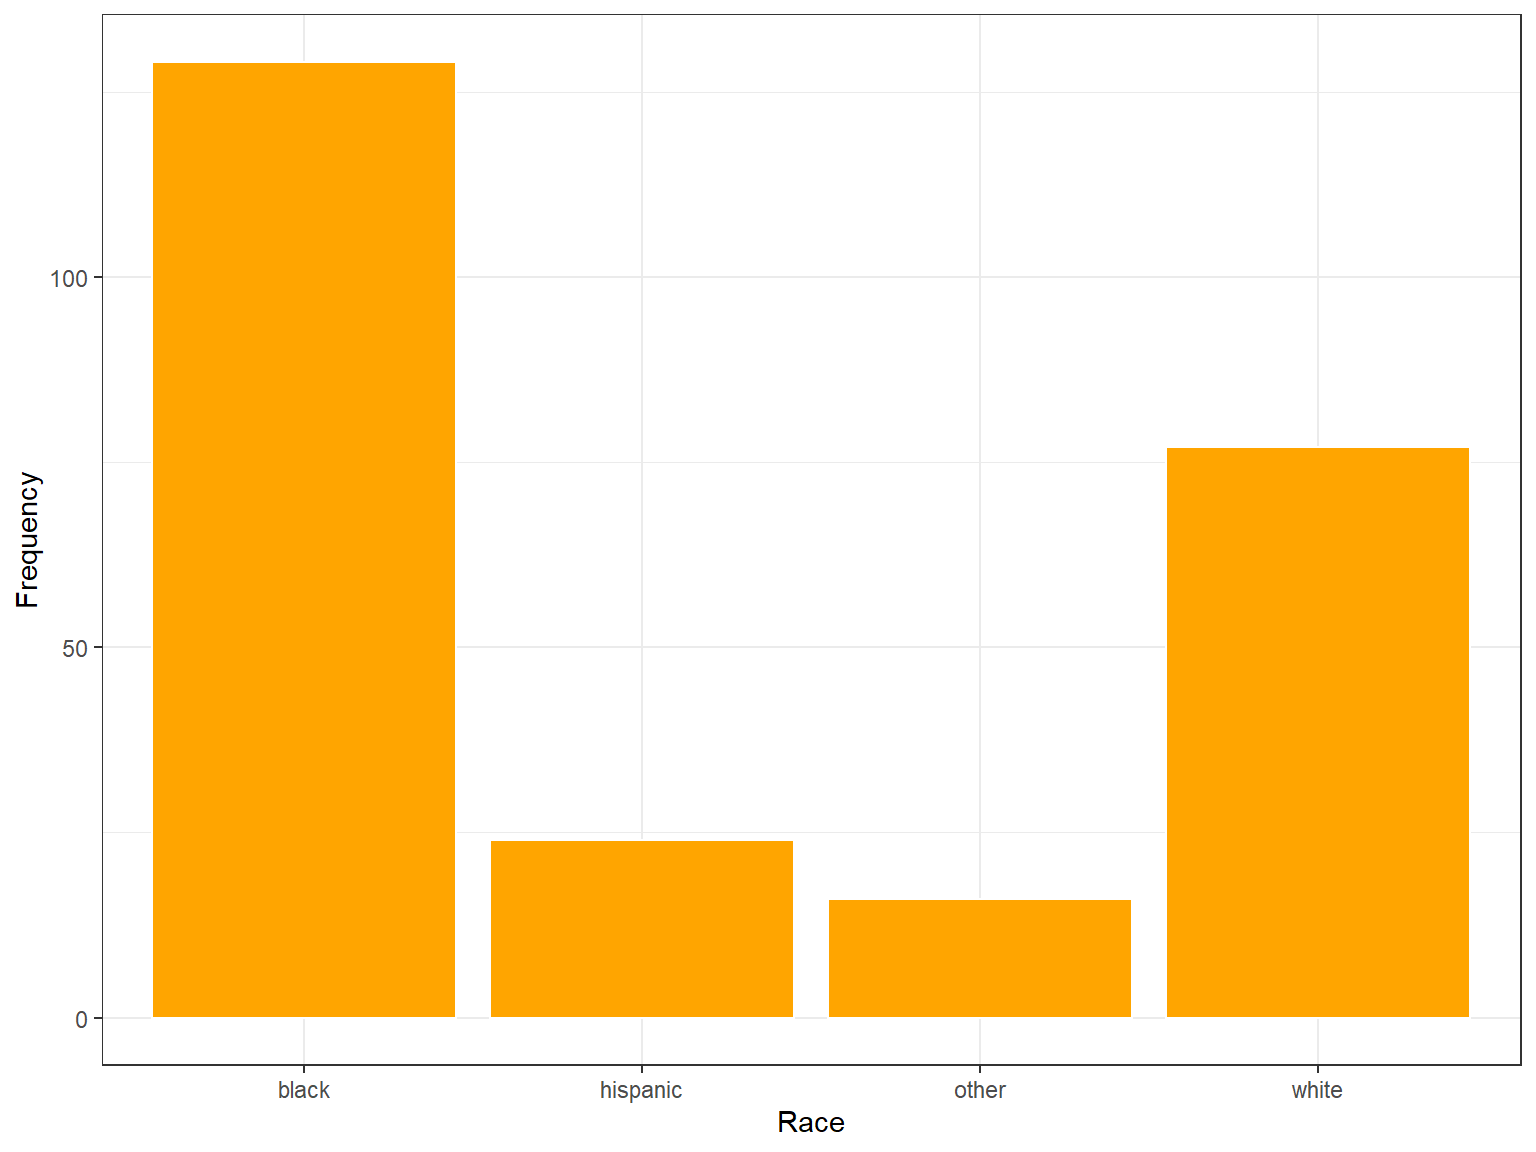
\includegraphics{rbook_files/figure-latex/ggbar1-1} 

}

\caption{A bar plot example with `ggplot2`}\label{fig:ggbar1}
\end{figure}

\begin{Shaded}
\begin{Highlighting}[]
\KeywordTok{ggplot}\NormalTok{(}\DataTypeTok{data =}\NormalTok{ medical, }
       \DataTypeTok{mapping =} \KeywordTok{aes}\NormalTok{(}\DataTypeTok{x =}\NormalTok{ race, }\DataTypeTok{fill =}\NormalTok{ sex)) }\OperatorTok{+}\StringTok{ }
\StringTok{  }\KeywordTok{labs}\NormalTok{(}\DataTypeTok{x =} \StringTok{"Race"}\NormalTok{,}
       \DataTypeTok{y =} \StringTok{"Frequency"}\NormalTok{) }\OperatorTok{+}\StringTok{ }
\StringTok{  }\KeywordTok{geom_bar}\NormalTok{() }\OperatorTok{+}
\StringTok{  }\KeywordTok{theme_bw}\NormalTok{()}
\end{Highlighting}
\end{Shaded}

\begin{figure}

{\centering 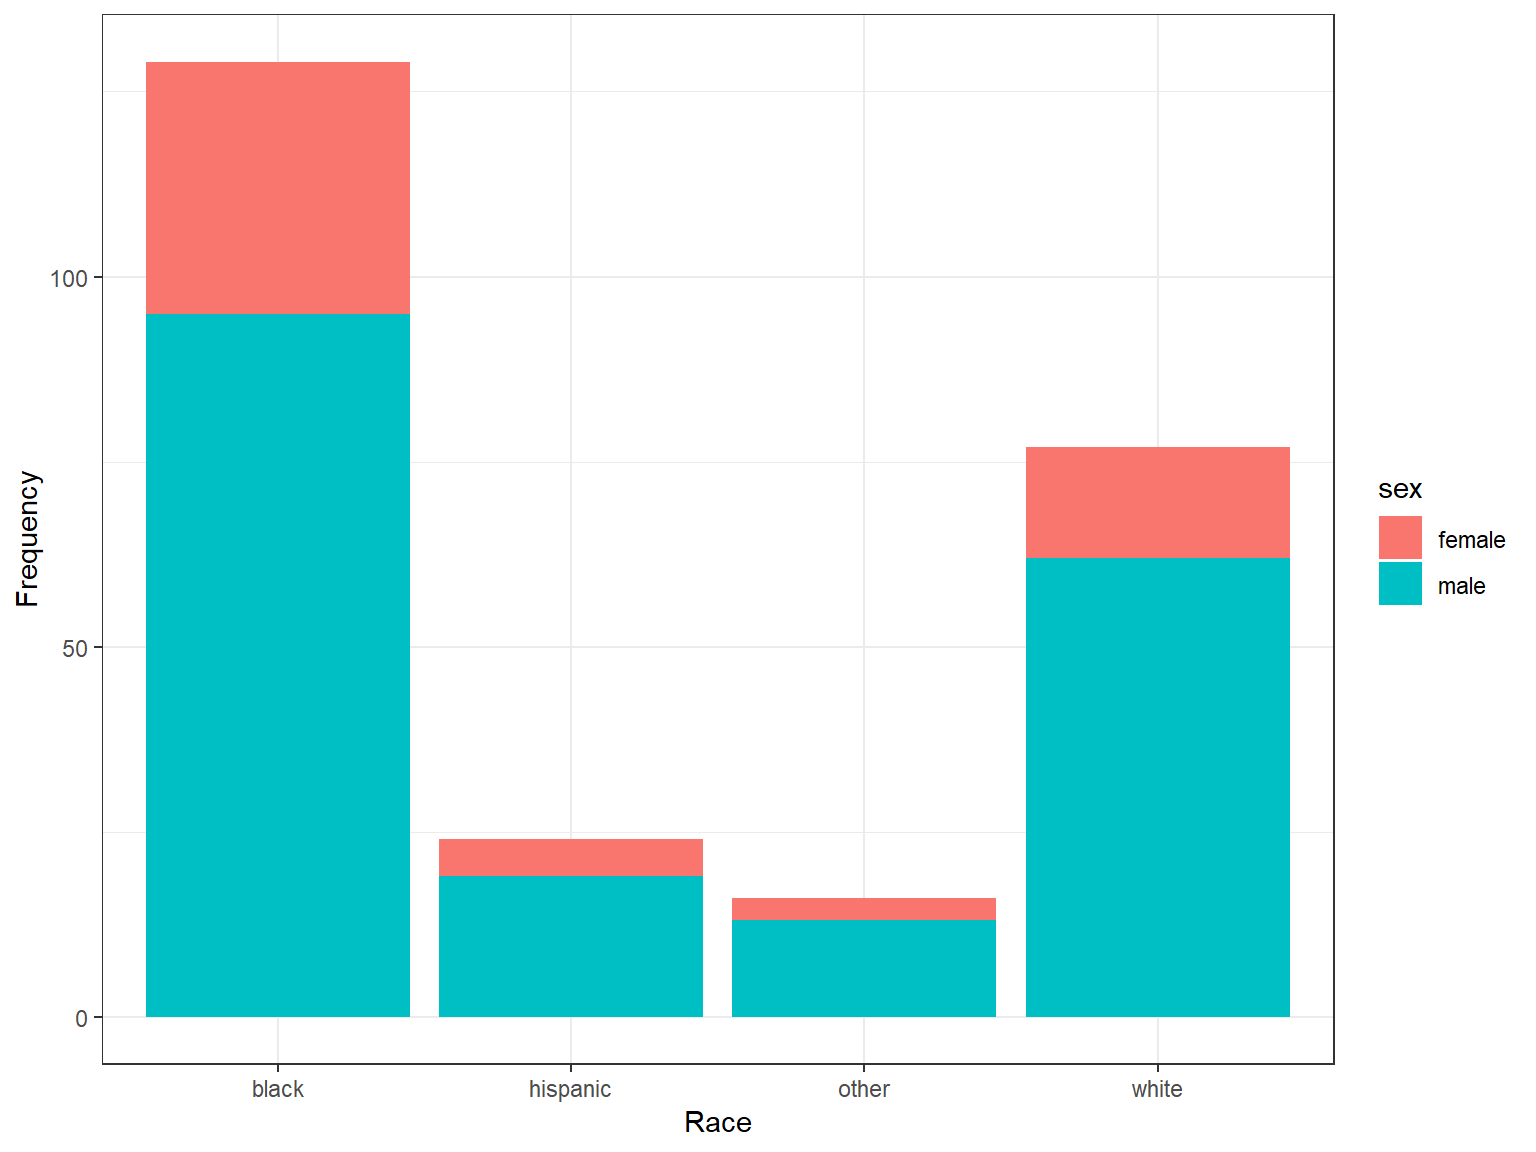
\includegraphics{rbook_files/figure-latex/ggbar2-1} 

}

\caption{A bar plot example with `ggplot2` (stacked bar chart)}\label{fig:ggbar2}
\end{figure}

\begin{Shaded}
\begin{Highlighting}[]
\KeywordTok{ggplot}\NormalTok{(}\DataTypeTok{data =}\NormalTok{ medical, }
       \DataTypeTok{mapping =} \KeywordTok{aes}\NormalTok{(}\DataTypeTok{x =}\NormalTok{ race, }\DataTypeTok{fill =}\NormalTok{ sex)) }\OperatorTok{+}\StringTok{ }
\StringTok{  }\KeywordTok{labs}\NormalTok{(}\DataTypeTok{x =} \StringTok{"Race"}\NormalTok{,}
       \DataTypeTok{y =} \StringTok{"Frequency"}\NormalTok{) }\OperatorTok{+}\StringTok{ }
\StringTok{  }\KeywordTok{geom_bar}\NormalTok{(}\DataTypeTok{position =} \StringTok{"dodge"}\NormalTok{) }\OperatorTok{+}
\StringTok{  }\KeywordTok{theme_bw}\NormalTok{()}
\end{Highlighting}
\end{Shaded}

\begin{figure}

{\centering 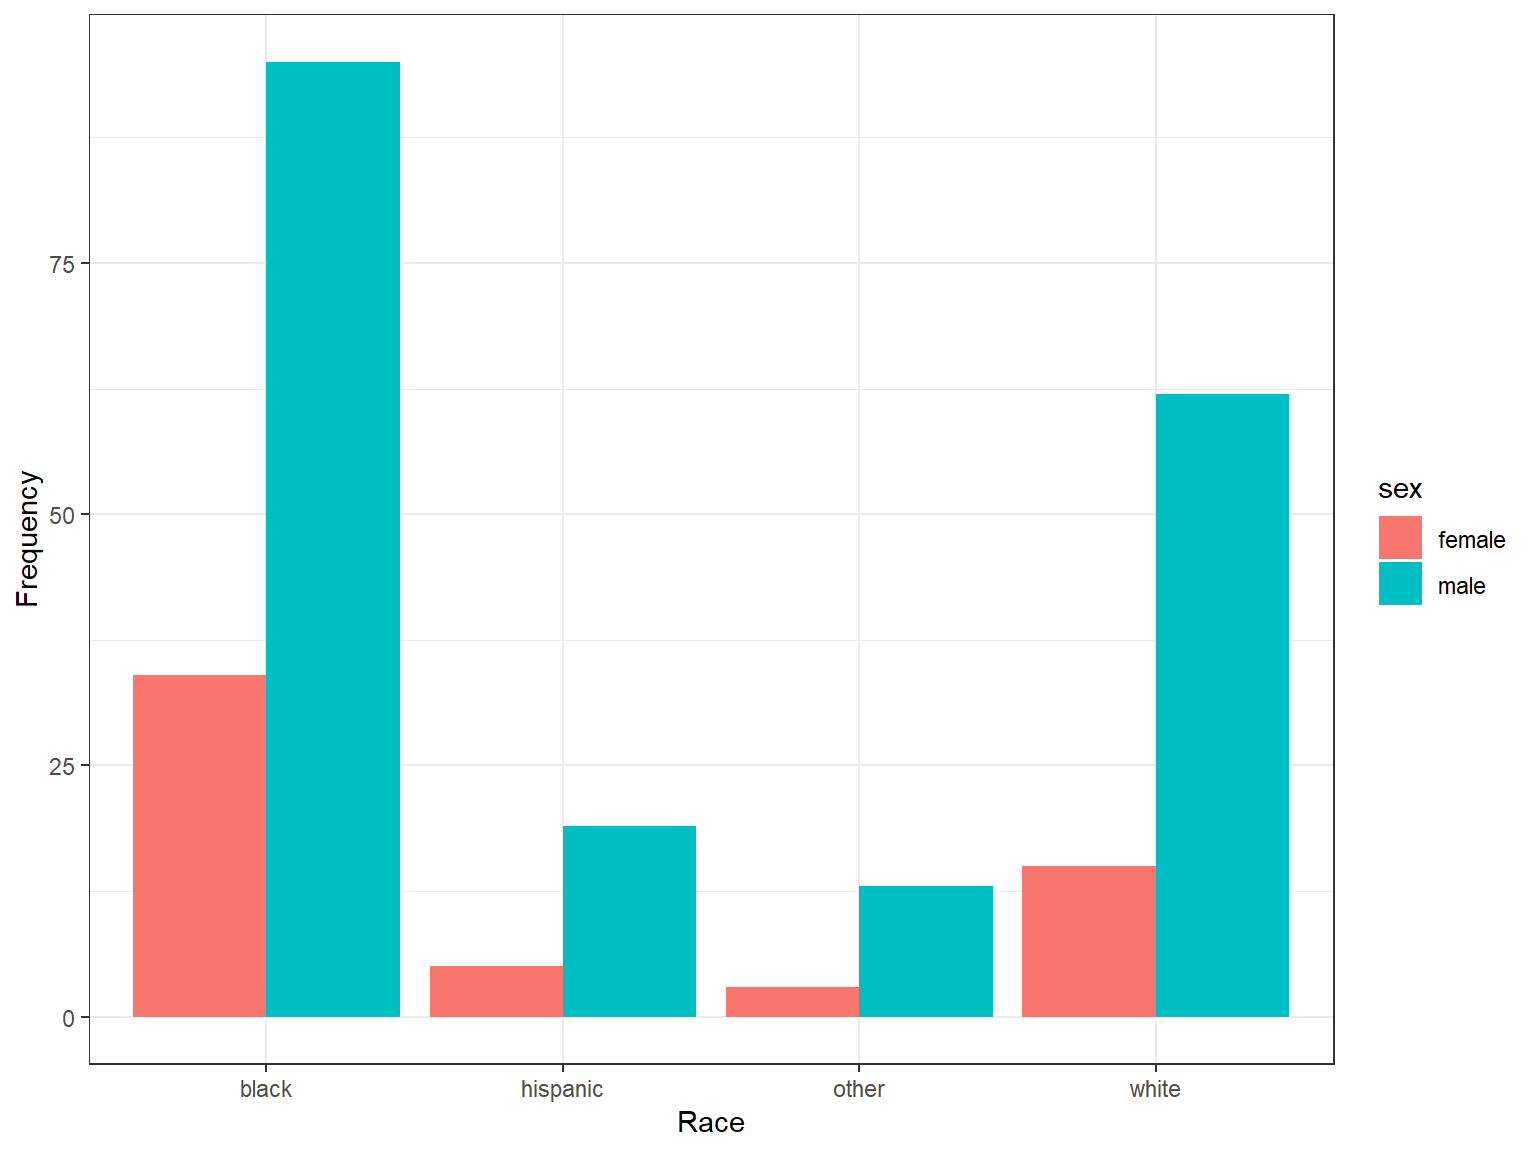
\includegraphics{rbook_files/figure-latex/ggbar3-1} 

}

\caption{A bar plot example with `ggplot2` (side-by-side bars)}\label{fig:ggbar3}
\end{figure}

\begin{Shaded}
\begin{Highlighting}[]
\KeywordTok{ggplot}\NormalTok{(}\DataTypeTok{data =}\NormalTok{ medical, }
       \DataTypeTok{mapping =} \KeywordTok{aes}\NormalTok{(}\DataTypeTok{x =}\NormalTok{ race, }\DataTypeTok{fill =}\NormalTok{ sex)) }\OperatorTok{+}\StringTok{ }
\StringTok{  }\KeywordTok{labs}\NormalTok{(}\DataTypeTok{x =} \StringTok{"Race"}\NormalTok{,}
       \DataTypeTok{y =} \StringTok{"Frequency"}\NormalTok{) }\OperatorTok{+}\StringTok{ }
\StringTok{  }\KeywordTok{geom_bar}\NormalTok{(}\DataTypeTok{position =} \StringTok{"dodge"}\NormalTok{) }\OperatorTok{+}
\StringTok{  }\KeywordTok{facet_wrap}\NormalTok{(}\OperatorTok{~}\StringTok{ }\NormalTok{sex, }\DataTypeTok{ncol =} \DecValTok{1}\NormalTok{) }\OperatorTok{+}
\StringTok{  }\KeywordTok{theme_bw}\NormalTok{()}
\end{Highlighting}
\end{Shaded}

\begin{figure}

{\centering 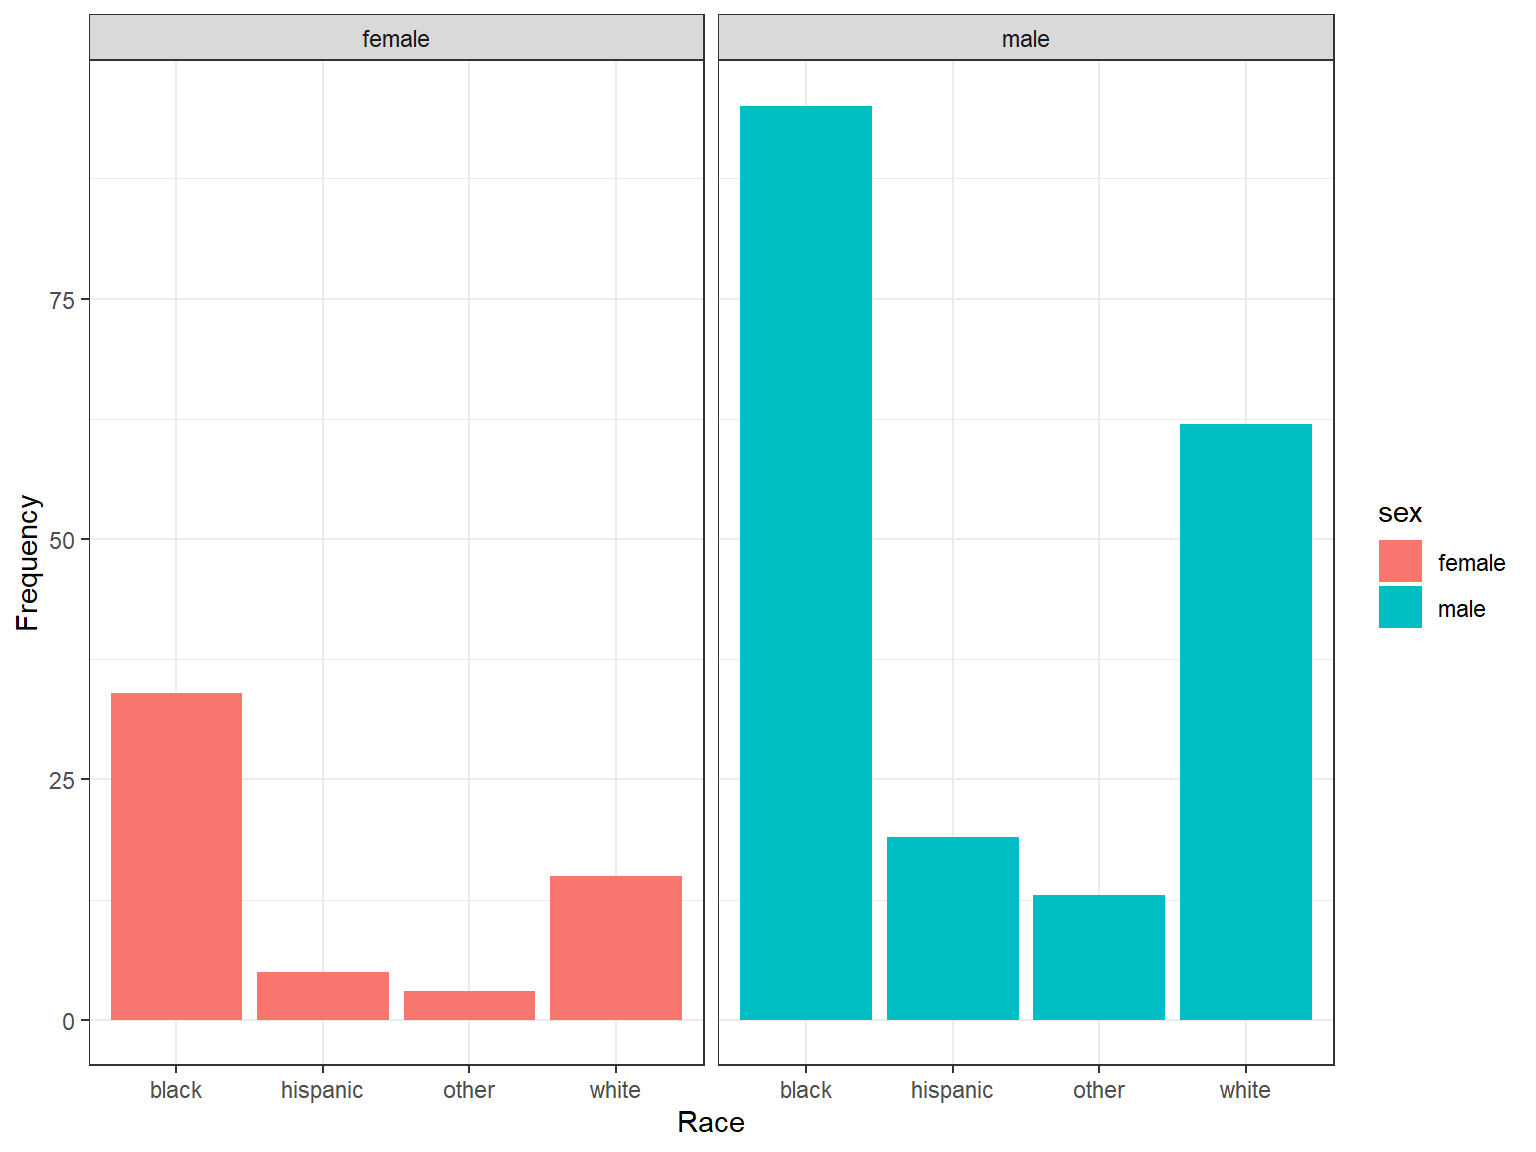
\includegraphics{rbook_files/figure-latex/ggbar4-1} 

}

\caption{A bar plot example with `ggplot2` (faceted)}\label{fig:ggbar4}
\end{figure}

\hypertarget{your-turn-7}{%
\subsection{Your Turn}\label{your-turn-7}}

Here you will create a scatterplot of \texttt{depression1} and \texttt{mental1} using \texttt{geom\_point()}, with

\begin{itemize}
\tightlist
\item
  point colours set by \texttt{sex} (i.e., \texttt{colour\ =\ sex})
\item
  faceted by \texttt{substance} (i.e., \texttt{facet\_wrap(\textasciitilde{}\ substance,\ ncol\ =\ 1)})
\end{itemize}

Do either \texttt{sex} or \texttt{substance} seem to differentiate the relationship between \texttt{depression1} and \texttt{mental1}?

\hypertarget{part5}{%
\chapter{Hypothesis Testing}\label{part5}}

\hypertarget{some-theory}{%
\section{Some Theory}\label{some-theory}}

\begin{quote}
Statistics cannot prove anything with certainty. Instead, the power of statistical inference derives from observing some pattern or outcome and then using probability to determine the most likely explanation for that outcome.\citep{Wheelan}
\end{quote}

In its most abstract form, hypothesis testing really a very simple idea: the researcher has some theory about the world, and wants to determine whether or not the data actually support that theory. However, the details are messy, and most people find the theory of hypothesis testing to be the most frustrating part of statistics. In hypothesis testing, we want to:

\begin{itemize}
\tightlist
\item
  explore whether parameters in a model take specified values or fall in certain ranges
\item
  detect significant differences, or differences that did not occur by random chance
\end{itemize}

To address these goals, we will use data from a sample to help us decide between two competing hypotheses about a population. These two completing hypotheses are:

\begin{itemize}
\tightlist
\item
  \textbf{a null hypothesis} (\(H_0\)) that corresponds to the exact opposite of what we want to prove
\item
  \textbf{an alternative hypothesis} (\(H_1\)) that represents what we actually believe.
\end{itemize}

The claim for which we seek significant evidence is assigned to the alternative hypothesis. The alternative is usually what the experimenter or researcher wants to establish or find evidence for. Usually, the null hypothesis is a claim that there really is ``no effect'' or ``no difference''. In many cases, the null hypothesis represents the status quo or that nothing interesting is happening.

For example, we can think of hypothesis testing in the same context as a criminal trial in the United States. A criminal trial in the United States is a familiar situation in which a choice between two contradictory claims must be made.

\begin{itemize}
\tightlist
\item
  The accuser of the crime must be judged either guilty or not guilty.
\item
  Under the U.S. system of justice, the individual on trial is initially presumed not guilty.
\item
  Only \emph{strong evidence} to the contrary causes the not guilty claim to be rejected in favor of a guilty verdict.
\end{itemize}

The phrase ``beyond a reasonable doubt'' is often used to set the cutoff value for when enough evidence has been given to convict. Theoretically, we should never say ``The person is innocent'' but instead ``There is not sufficient evidence to show that the person is guilty''. That is, technically it is \textbf{not} correct to say that we accept the null hypothesis. Accepting the null hypothesis is the same as saying that a person is innocent. We cannot show that a person is innocent; we can only say that there was not enough substantial evidence to find the person guilty.

\hypertarget{types-of-inferential-statistics}{%
\section{Types of Inferential Statistics}\label{types-of-inferential-statistics}}

We assess the strength of evidence by assuming the null hypothesis is true and determining how unlikely it would be to see sample statistics as extreme (or more extreme) as those in the original sample. Using inferential statistics allows us to make predictions or inferences about a population from observations based on a sample. We can calculate several inferential statistics:

\begin{enumerate}
\def\labelenumi{\arabic{enumi}.}
\tightlist
\item
  Whether a sample mean is equal to a particular value:

  \begin{itemize}
  \tightlist
  \item
    One sample t-test (\(H_0: \mu=\text{value}\))
  \end{itemize}
\item
  Whether two sample means are equal:

  \begin{itemize}
  \tightlist
  \item
    Independent samples t-test (\(H_0: \mu_1=\mu_2\) or \(H_0: \mu_1-\mu_2=0\))
  \item
    Repeated measures t-test (\(H_0: \mu_D=0\) or \(H_0: \mu_1-\mu_2=0\))
  \end{itemize}
\item
  Whether three or more groups have equal means:

  \begin{itemize}
  \tightlist
  \item
    ANOVA (\(H_0: \mu_1=\mu_2=\mu_3=\dots=\mu_k\))
  \end{itemize}
\end{enumerate}

\hypertarget{one-sample-t-test}{%
\section{\texorpdfstring{One-Sample \(t\) Test}{One-Sample t Test}}\label{one-sample-t-test}}

Suppose we wish to test for the population mean (\(\mu\)) using a dataset of size (\(n\)), and the population standard deviation (\(\sigma\)) is not known. We want to test the null hypothesis \(H_0:\mu = \mu_0\) against some alternative hypothesis, with (\(\alpha\)) level of significance.

The test statistic will be:

\[t = \frac{\bar{x} - \mu_0}{\frac{S}{\sqrt{n}}}\]

with \(df = n - 1\) degrees of freedom. In the formula:

\begin{itemize}
\tightlist
\item
  \(\bar{x}\) is the sample mean
\item
  \(\mu_0\) is the population mean that we are comparing against our sample mean
\item
  \(S\) is the sample standard deviation
\item
  \(n\) is the sample size
\end{itemize}

If \(t > t_{critical}\) at the \(\alpha\) level of significance, we reject the null hypothesis; otherwise we \emph{retain} the null hypothesis.

\hypertarget{example}{%
\subsection{Example}\label{example}}

Let's see one-sample t-test in action. All the patients in the \texttt{medical} dataset received a mental test at the baseline (when they were accepted to the study). The researcher who created the mental test reported that the mean score on this test for people with no mental issues should be around 35. Now we want to know whether the mean mental test for our sample of patients differs from the mean mental test score for the general population. Our hypotheses are:

\begin{itemize}
\tightlist
\item
  \(H_0: \mu = 35\)
\item
  \(H_1: \mu \neq 35\)
\end{itemize}

\begin{Shaded}
\begin{Highlighting}[]
\CommentTok{# Let's see the mean for mental1 in the data}
\KeywordTok{mean}\NormalTok{(medical}\OperatorTok{$}\NormalTok{mental1) }\CommentTok{# it is 31.68}
\end{Highlighting}
\end{Shaded}

\begin{verbatim}
[1] 31.68
\end{verbatim}

It looks like our sample mean is less than the population mean of 35. But, the question is whether it is small enough to conclude that there is a statistically significant difference between the sample mean (i.e., 31.68) and the population mean (i.e., 35).

\begin{Shaded}
\begin{Highlighting}[]
\KeywordTok{t.test}\NormalTok{(medical}\OperatorTok{$}\NormalTok{mental1, }\DataTypeTok{mu =} \DecValTok{35}\NormalTok{, }\DataTypeTok{conf.level =} \FloatTok{0.95}\NormalTok{, }\DataTypeTok{alternative =} \StringTok{"two.sided"}\NormalTok{)}
\end{Highlighting}
\end{Shaded}

\begin{verbatim}

    One Sample t-test

data:  medical$mental1
t = -4.2, df = 240, p-value = 4e-05
alternative hypothesis: true mean is not equal to 35
95 percent confidence interval:
 30.11 33.25
sample estimates:
mean of x 
    31.68 
\end{verbatim}

The \texttt{lsr} package \citep{R-lsr} does the same analysis and it provides more organized output:

\begin{Shaded}
\begin{Highlighting}[]
\CommentTok{# Install the activate the package}
\KeywordTok{install.packages}\NormalTok{(}\StringTok{"lsr"}\NormalTok{)}
\KeywordTok{library}\NormalTok{(}\StringTok{"lsr"}\NormalTok{)}

\CommentTok{# Run one-sample t test}
\KeywordTok{oneSampleTTest}\NormalTok{(}\DataTypeTok{x=}\NormalTok{medical}\OperatorTok{$}\NormalTok{mental1, }\DataTypeTok{mu=}\DecValTok{35}\NormalTok{, }\DataTypeTok{conf.level=}\FloatTok{0.95}\NormalTok{, }\DataTypeTok{one.sided=}\OtherTok{FALSE}\NormalTok{)}
\end{Highlighting}
\end{Shaded}

\begin{verbatim}

   One sample t-test 

Data variable:   medical$mental1 

Descriptive statistics: 
            mental1
   mean      31.680
   std dev.  12.486

Hypotheses: 
   null:        population mean equals 35 
   alternative: population mean not equal to 35 

Test results: 
   t-statistic:  -4.17 
   degrees of freedom:  245 
   p-value:  <.001 

Other information: 
   two-sided 95% confidence interval:  [30.112, 33.248] 
   estimated effect size (Cohen's d):  0.266 
\end{verbatim}

\textbf{Conclusion:} With the significance level of \(\alpha=.05\), we reject the null hypothesis that the average mental score in the \texttt{medical} dataset is the same as the average mental score in the population, \(t(240)=-4.2\), \(p < .001\), \(CI_{95}=[30.11, 33.25]\).

\hypertarget{independent-samples-t-test}{%
\section{\texorpdfstring{Independent-Samples \(t\) Test}{Independent-Samples t Test}}\label{independent-samples-t-test}}

Suppose we have data from two independent populations, \(x_1 \sim N(\mu_{x_1}, \sigma_{x_1})\) and \(x_2 \sim N(\mu_{x_2}, \sigma_{x_2})\). We wish to determine whether the two population means, \(\mu_{x_1}\) and \(\mu_{x_2}\), are the same or different. We want to test the null hypothesis \(H_0: \mu_{X_1} = \mu_{X_2}\) against some alternative hypothesis, with \(\alpha\) level of significance. The test statistic will be:

\[t =\dfrac{ (\bar{x}_1 - \bar{x}_2)}{ \sqrt{\dfrac{{S_p}^2}{n_1} + \dfrac{{S_p}^2}{n_2}}  }\]

and

\[S_p = \frac{(n_1-1)S_1^2 + (n_2-1)S_2^2}{n_1+n_2-2}\]

with \(df = n_1 + n_2 - 2\) degrees of freedom. In the formula:

\begin{itemize}
\tightlist
\item
  \(\bar{x}_1\) is the sample mean response of the first group
\item
  \(\bar{x}_2\) is the sample mean response of the second group
\item
  \(S_1^2\) is the sample variance of the response of the first group
\item
  \(S_2^2\) is the sample variance of the response of the second group
\item
  \(S_p\) is the pooled variance
\item
  \(n_1\) is the sample size of the first group
\item
  \(n_2\) is the sample size of the second group
\end{itemize}

If \(t > t_{critical}\) at the \(\alpha\) level of significance, we reject the null hypothesis; otherwise we \emph{retain} the null hypothesis.

\hypertarget{example-1}{%
\subsection{Example}\label{example-1}}

Using the \texttt{medical} dataset, we want to know whether there was a significant difference between male and female patients' depression levels at the baseline. We will use \texttt{sex} and \texttt{depression1} to investigate this question. Before we test this question, let's see the boxplot for these two groups:

\begin{Shaded}
\begin{Highlighting}[]
\KeywordTok{boxplot}\NormalTok{(}\DataTypeTok{formula =}\NormalTok{ depression1 }\OperatorTok{~}\StringTok{ }\NormalTok{sex,}
        \DataTypeTok{data =}\NormalTok{ medical,}
        \DataTypeTok{main =} \StringTok{"Depression Scores by Sex"}\NormalTok{,}
        \DataTypeTok{ylab =} \StringTok{"Depression at the baseline"}\NormalTok{,}
        \DataTypeTok{names =} \KeywordTok{c}\NormalTok{(}\StringTok{"Female"}\NormalTok{, }\StringTok{"Male"}\NormalTok{))}
\end{Highlighting}
\end{Shaded}

\begin{figure}

{\centering 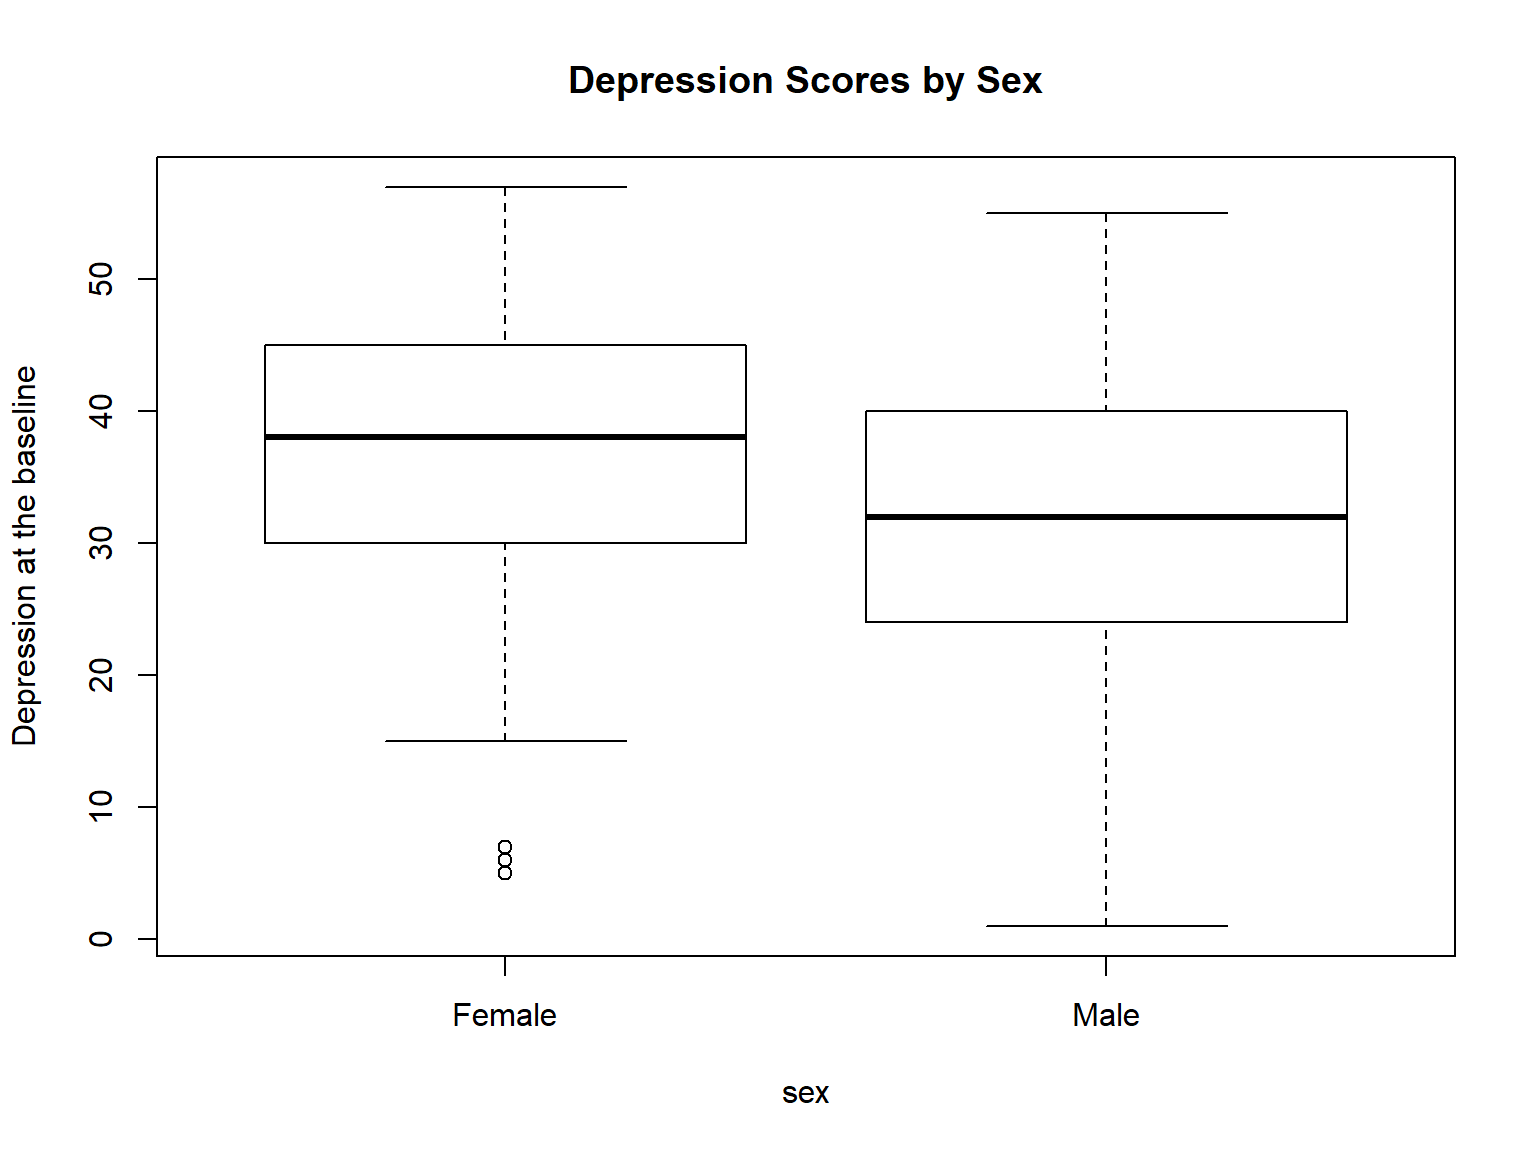
\includegraphics{rbook_files/figure-latex/boxplot5-1} 

}

\caption{Boxplot of depression scores by sex}\label{fig:boxplot5}
\end{figure}

It seems that female patients have higher levels of depression on average, compared to male patients. Next, we will create two new small datasets (\texttt{male} and \texttt{female}) that consist of only depression scores for each gender group.

\begin{Shaded}
\begin{Highlighting}[]
\NormalTok{male <-}\StringTok{ }\KeywordTok{subset}\NormalTok{(medical, sex }\OperatorTok{==}\StringTok{ "male"}\NormalTok{, }\DataTypeTok{select =} \StringTok{"depression1"}\NormalTok{)}
\NormalTok{female <-}\StringTok{ }\KeywordTok{subset}\NormalTok{(medical, sex }\OperatorTok{==}\StringTok{ "female"}\NormalTok{, }\DataTypeTok{select =} \StringTok{"depression1"}\NormalTok{)}
\KeywordTok{t.test}\NormalTok{(male, female, }\DataTypeTok{conf.level =} \FloatTok{0.95}\NormalTok{, }\DataTypeTok{alternative =} \StringTok{"two.sided"}\NormalTok{)}
\end{Highlighting}
\end{Shaded}

\begin{verbatim}

    Welch Two Sample t-test

data:  male and female
t = -2.5, df = 87, p-value = 0.02
alternative hypothesis: true difference in means is not equal to 0
95 percent confidence interval:
 -8.418 -0.928
sample estimates:
mean of x mean of y 
    31.50     36.18 
\end{verbatim}

We can again use the \texttt{lsr} package to get a better output. \texttt{independentSamplesTTest} function does not require us to separate the dataset for each group. We only need to specify the group variable, which is \texttt{sex} in our example. The only thing we need to make sure that the group variable is a factor.

\begin{Shaded}
\begin{Highlighting}[]
\NormalTok{medical}\OperatorTok{$}\NormalTok{sex <-}\StringTok{ }\KeywordTok{as.factor}\NormalTok{(medical}\OperatorTok{$}\NormalTok{sex)}

\KeywordTok{independentSamplesTTest}\NormalTok{(}\DataTypeTok{formula =}\NormalTok{ depression1 }\OperatorTok{~}\StringTok{ }\NormalTok{sex, }
                        \DataTypeTok{conf.level =} \FloatTok{0.95}\NormalTok{,}
                        \DataTypeTok{one.sided =} \OtherTok{FALSE}\NormalTok{, }
                        \DataTypeTok{data =}\NormalTok{ medical)}
\end{Highlighting}
\end{Shaded}

\begin{verbatim}

   Welch's independent samples t-test 

Outcome variable:   depression1 
Grouping variable:  sex 

Descriptive statistics: 
            female   male
   mean     36.175 31.503
   std dev. 12.675 11.758

Hypotheses: 
   null:        population means equal for both groups
   alternative: different population means in each group

Test results: 
   t-statistic:  2.48 
   degrees of freedom:  87.09 
   p-value:  0.015 

Other information: 
   two-sided 95% confidence interval:  [0.928, 8.418] 
   estimated effect size (Cohen's d):  0.382 
\end{verbatim}

\textbf{Conclusion:} With the significance level of \(\alpha=.05\), we reject the null hypothesis that the average depression score for male and female patients is the same in the population, \(t(87)=-2.5\), \(p < .05\), \(CI_{95}=[-8.42, -0.93]\).

\hypertarget{t-test-with-paired-data}{%
\section{\texorpdfstring{\(t\)-test with Paired Data}{t-test with Paired Data}}\label{t-test-with-paired-data}}

Suppose we have paired data, \(X_1\) and \(X_2\) with \(D=X_1-X_2 \sim N(\mu_D, \sigma)\). We wish to determine whether the two population means (or a single population across two time points), \(\mu_{X_1}\) and \(\mu_{X_2}\), are the same (i.e., \(\mu_D = 0\)) or different (i.e., \(\mu_D \neq 0\)). We test the null hypothesis \(H_0: \mu_X = \mu_Y\) against some alternative hypothesis, with \(\alpha\) level of significance. The test statistic will be:

\[t = \frac{\bar{D}}{\frac{S_D}{\sqrt{n}}}\]

with \(df = n -1\) degrees of freedom. In the formula:

\begin{itemize}
\tightlist
\item
  \(D\) is the difference between two populations (or two time points)
\item
  \(S_D\) is the sample standard deviation of the difference
\item
  \(n\) is the sample size of the second group
\end{itemize}

If \(t > t_{critical}\) at the \(\alpha\) level of significance, we reject the null hypothesis; otherwise we \emph{retain} the null hypothesis.

\hypertarget{example-2}{%
\subsection{Example}\label{example-2}}

Using the \texttt{medical} dataset, this time we want to know whether patients' depression scores at the baseline (\texttt{depression1}) are the same as their depression scores after 6 months (\texttt{depression2}). First, let's see the means for the two variables.

\begin{Shaded}
\begin{Highlighting}[]
\KeywordTok{mean}\NormalTok{(medical}\OperatorTok{$}\NormalTok{depression1)}
\end{Highlighting}
\end{Shaded}

\begin{verbatim}
[1] 32.59
\end{verbatim}

\begin{Shaded}
\begin{Highlighting}[]
\KeywordTok{mean}\NormalTok{(medical}\OperatorTok{$}\NormalTok{depression2)}
\end{Highlighting}
\end{Shaded}

\begin{verbatim}
[1] 22.72
\end{verbatim}

It seems that the scores at month 6 are much lower. Let's see if the difference is statistically significant.

\begin{Shaded}
\begin{Highlighting}[]
\KeywordTok{t.test}\NormalTok{(medical}\OperatorTok{$}\NormalTok{depression1, medical}\OperatorTok{$}\NormalTok{depression2, }
       \DataTypeTok{paired =} \OtherTok{TRUE}\NormalTok{, }\DataTypeTok{alternative =} \StringTok{"two.sided"}\NormalTok{,}
       \DataTypeTok{conf.level =} \FloatTok{0.95}\NormalTok{)}
\end{Highlighting}
\end{Shaded}

\begin{verbatim}

    Paired t-test

data:  medical$depression1 and medical$depression2
t = 11, df = 240, p-value <2e-16
alternative hypothesis: true difference in means is not equal to 0
95 percent confidence interval:
  8.021 11.719
sample estimates:
mean of the differences 
                   9.87 
\end{verbatim}

Let's repeat the same analysis with the \texttt{lsr} package.

\begin{Shaded}
\begin{Highlighting}[]
\KeywordTok{pairedSamplesTTest}\NormalTok{(}\DataTypeTok{formula =} \OperatorTok{~}\StringTok{ }\NormalTok{depression1 }\OperatorTok{+}\StringTok{ }\NormalTok{depression2,}
                   \DataTypeTok{conf.level =} \FloatTok{0.95}\NormalTok{,}
                   \DataTypeTok{one.sided =} \OtherTok{FALSE}\NormalTok{, }
                   \DataTypeTok{data =}\NormalTok{ medical)}
\end{Highlighting}
\end{Shaded}

\begin{verbatim}

   Paired samples t-test 

Variables:  depression1 , depression2 

Descriptive statistics: 
            depression1 depression2 difference
   mean          32.585      22.715      9.870
   std dev.      12.112      14.287     14.727

Hypotheses: 
   null:        population means equal for both measurements
   alternative: different population means for each measurement

Test results: 
   t-statistic:  10.51 
   degrees of freedom:  245 
   p-value:  <.001 

Other information: 
   two-sided 95% confidence interval:  [8.021, 11.719] 
   estimated effect size (Cohen's d):  0.67 
\end{verbatim}

\textbf{Conclusion:} With the significance level of \(\alpha=.05\), we reject the null hypothesis that the average depression scores for the baseline and 6th month are the same in the population, \(t(245)=10.51\), \(p < .001\), \(CI_{95}=[8.02, 11.72]\).

\hypertarget{analysis-of-variance-anova}{%
\section{Analysis of Variance (ANOVA)}\label{analysis-of-variance-anova}}

Independent-samples \(t\)-test that we have seen earlier is suitable for comparing the means of two independent groups. But, what if there are more than two groups to compare? One could suggest that we run multiple \(t\)-tests to compare all possible pairs and make a decision at the end. However, each statistical test that we run involves a certain level of error (known as Type I error) that leads to incorrect conclusions on the results. Repeating several \(t\)-tests to compare the groups would increase the likelihood of making incorrect conclusions. Therefore, when there are three or more groups to be compared, we follow a procedure called Analysis of Variance -- or shortly ANOVA.

Suppose we have \(K\) number of populations. Collect a random sample of size \(n_1\) from population 1, \(n_2\) from population 2, \ldots{}, \(n_K\) from population \(k\). We assume all populations have the same standard deviation (and they are normally distributed). We wish to test the following null hypothesis:

\[H_0: \mu_1=\mu_2=\mu_3=\dots=\mu_K\]
against

\[H_1: H_0 \text{ is false}\]

which means that all of the groups would have equal means in their populations. If at least one of the groups has a significantly different mean, then we would reject the null hypothesis and run post-hoc tests to find out which group(s) are different.

Let \(N = \sum_{k = 1}^{K} n_k\) be the grand total, \((\overline{x}_k = \frac{1}{n_k} \sum_{i = 1}^{n_k} x_{ki}\)) be the sample mean for sample \(k\), and \(\overline{x}_{\cdot} = \frac{1}{N} \sum_{k = 1}^{K} \sum_{i = 1}^{n_k} x_{ki}\) be the grand mean. Then, the \(F\)-statistic is

\[F = \frac{\sum_{k = 1}^{K}\left(\overline{x}_k - \overline{x}_{\cdot}\right)^2/(K - 1)}{\sum_{k = 1}^{K} \sum_{i = 1}^{n_k} \left(x_{ki} - \overline{x}_k\right)^2/(N - K)}\]

with degrees of freedom of \(df_1 = K - 1\) and \(df_2 = N - K\).

If \(F > F_{critical}\) at the \(\alpha\) level of significance, we reject the null hypothesis; otherwise we \emph{retain} the null hypothesis.

\hypertarget{example-3}{%
\subsection{Example}\label{example-3}}

Using the \texttt{medical} dataset, we want to investigate whether patients with different types of substance addition had the same level of depression at the baseline. We will use \texttt{depression1} and \texttt{substance} for this analysis. Before we begin the analysis, let's visualize the distribution of \texttt{depression1} by \texttt{substance} to get a sense of potential group differences.

\begin{Shaded}
\begin{Highlighting}[]
\KeywordTok{boxplot}\NormalTok{(}\DataTypeTok{formula =}\NormalTok{ depression1 }\OperatorTok{~}\StringTok{ }\NormalTok{substance,}
        \DataTypeTok{data =}\NormalTok{ medical,}
        \DataTypeTok{main =} \StringTok{"Depression Scores by Substance Type"}\NormalTok{,}
        \DataTypeTok{ylab =} \StringTok{"Depression at the baseline"}\NormalTok{)}
\end{Highlighting}
\end{Shaded}

\begin{figure}

{\centering 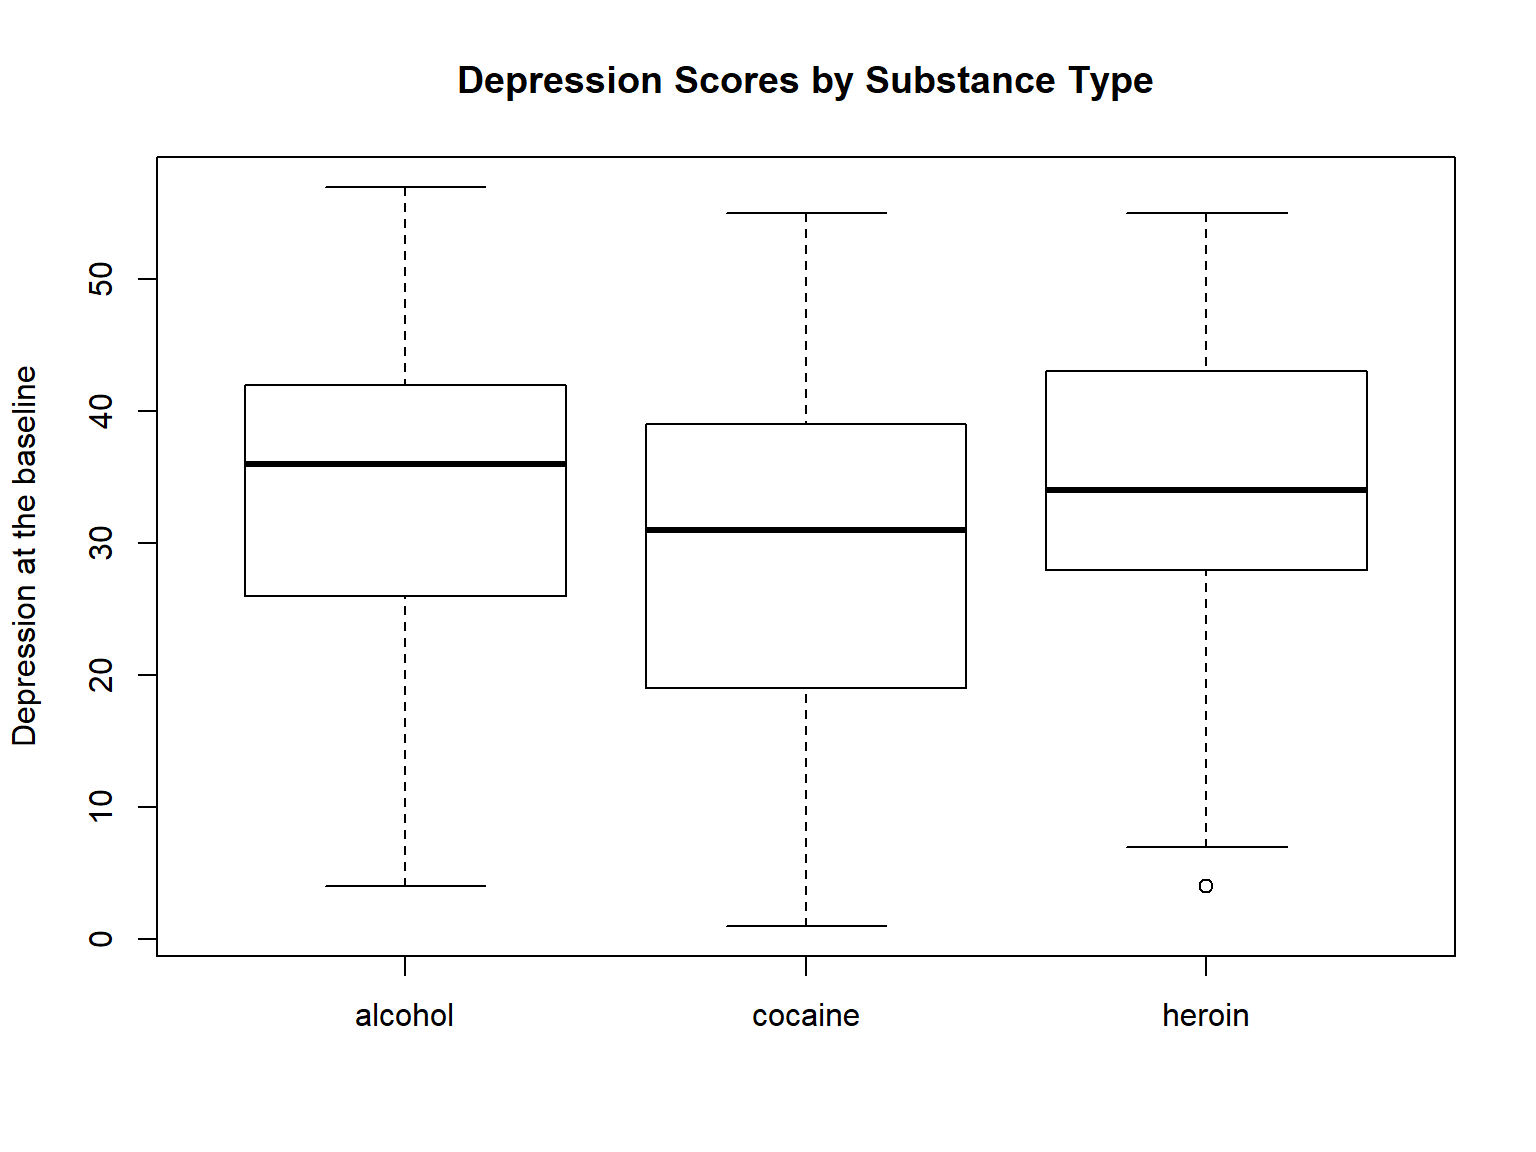
\includegraphics{rbook_files/figure-latex/boxplot6-1} 

}

\caption{Boxplot of depression scores by substance type}\label{fig:boxplot6}
\end{figure}

The boxplot shows that the means are close across the three groups but we cannot tell for sure if the differences are negligible to ignore. We will use the \texttt{aov} function -- which is part of base \textbf{R}.

\begin{Shaded}
\begin{Highlighting}[]
\CommentTok{# Compute the analysis of variance}
\NormalTok{aov_model1 <-}\StringTok{ }\KeywordTok{aov}\NormalTok{(depression1 }\OperatorTok{~}\StringTok{ }\NormalTok{substance, }\DataTypeTok{data =}\NormalTok{ medical)}

\CommentTok{# Summary of the analysis}
\KeywordTok{summary}\NormalTok{(aov_model1)}
\end{Highlighting}
\end{Shaded}

\begin{verbatim}
             Df Sum Sq Mean Sq F value Pr(>F)  
substance     2   1209     605    4.23  0.016 *
Residuals   243  34733     143                 
---
Signif. codes:  0 '***' 0.001 '**' 0.01 '*' 0.05 '.' 0.1 ' ' 1
\end{verbatim}

\textbf{Conclusion:} With the significance level of \(\alpha=.05\), the output shows that \(F(2, 243) = 4.23, p < .05\), indicating that the test is statistically significant and thus we need to reject the null hypothesis of equal group means. This finding also suggests that at least one of the groups is different from the others.

As the ANOVA test is significant, now we can compute Tukey HSD (Tukey Honest Significant Differences) for performing multiple pairwise-comparison between the means of groups. The function \texttt{TukeyHD()} takes the fitted ANOVA as an argument and gives us the pairwise-comparison results.

\begin{Shaded}
\begin{Highlighting}[]
\KeywordTok{TukeyHSD}\NormalTok{(aov_model1)}
\end{Highlighting}
\end{Shaded}

\begin{verbatim}
  Tukey multiple comparisons of means
    95% family-wise confidence level

Fit: aov(formula = depression1 ~ substance, data = medical)

$substance
                    diff     lwr     upr  p adj
cocaine-alcohol -4.62684 -8.7730 -0.4807 0.0245
heroin-alcohol  -0.08964 -4.7249  4.5456 0.9989
heroin-cocaine   4.53720 -0.1281  9.2025 0.0586
\end{verbatim}

In the output above,

\begin{itemize}
\tightlist
\item
  \textbf{diff:} difference between means of the two groups
\item
  \textbf{lwr, upr:} the lower and the upper end point of the confidence interval at 95\%
\item
  \textbf{p adj:} p-value after adjustment for the multiple comparisons
\end{itemize}

It can be seen from the output that only the difference between cocaine and alcohol is significant with an adjusted p-value of 0.0245.

We can add other variables into the ANOVA model and continue testing. Let's include \texttt{sex} as a second variable.

\begin{Shaded}
\begin{Highlighting}[]
\CommentTok{# Substance + Sex}
\NormalTok{aov_model2 <-}\StringTok{ }\KeywordTok{aov}\NormalTok{(depression1 }\OperatorTok{~}\StringTok{ }\NormalTok{substance }\OperatorTok{+}\StringTok{ }\NormalTok{sex, }\DataTypeTok{data =}\NormalTok{ medical)}
\KeywordTok{summary}\NormalTok{(aov_model2)}
\end{Highlighting}
\end{Shaded}

\begin{verbatim}
             Df Sum Sq Mean Sq F value Pr(>F)   
substance     2   1209     605    4.36 0.0138 * 
sex           1   1199    1199    8.65 0.0036 **
Residuals   242  33534     139                  
---
Signif. codes:  0 '***' 0.001 '**' 0.01 '*' 0.05 '.' 0.1 ' ' 1
\end{verbatim}

\begin{Shaded}
\begin{Highlighting}[]
\CommentTok{# Substance + Sex + Substance x Sex}
\NormalTok{aov_model3 <-}\StringTok{ }\KeywordTok{aov}\NormalTok{(depression1 }\OperatorTok{~}\StringTok{ }\NormalTok{substance}\OperatorTok{*}\NormalTok{sex, }\DataTypeTok{data =}\NormalTok{ medical)}
\KeywordTok{summary}\NormalTok{(aov_model3)}
\end{Highlighting}
\end{Shaded}

\begin{verbatim}
               Df Sum Sq Mean Sq F value Pr(>F)   
substance       2   1209     605    4.38 0.0135 * 
sex             1   1199    1199    8.69 0.0035 **
substance:sex   2    435     218    1.58 0.2083   
Residuals     240  33098     138                  
---
Signif. codes:  0 '***' 0.001 '**' 0.01 '*' 0.05 '.' 0.1 ' ' 1
\end{verbatim}

The output shows that \texttt{sex} is also statistically significant in the model; but the interaction of \texttt{sex} and \texttt{substance} is not statisticall significant.

\hypertarget{your-turn-8}{%
\subsection{Your Turn}\label{your-turn-8}}

Now you will run several hypothesis tests using the variables in the \texttt{medical} dataset:

\begin{enumerate}
\def\labelenumi{\arabic{enumi}.}
\item
  Run an independent-samples \(t\)-test where you will investigate whether the average depression scores at the baseline (i.e., \texttt{depression1}) are the same for suicidal patients (i.e., \texttt{suicial\ ==\ "yes"}) and non-suicidal patients (i.e., \texttt{suicial\ ==\ "no"}).
\item
  You will conduct a paired \(t\)-test to investigate whether patients' average mental scores at the baseline (i.e., \texttt{mental1}) and their mental scores after 6 months (i.e., \texttt{mental2}) are the same.
\item
  You will conduct an ANOVA analysis to investigate whether the patients' physical scores at the baseline (i.e., \texttt{physical1}) differ depending on their race (i.e., \texttt{race}).
\end{enumerate}

\textbf{Note:} For the first and third hypothesis tests, draw a boxplot to identify potential mean differences before you begin your analysis.

\hypertarget{part6}{%
\chapter{Correlation and Regression}\label{part6}}

\hypertarget{correlation}{%
\section{Correlation}\label{correlation}}

Correlation measures the degree to which two variables are related to or associated with each other. It provides information on the strength and direction of relationships. The most widely used correlation index, also known as Pearson correlation, is

\[\text{For populations: } \rho = \frac{\sigma_{xy}}{\sigma_x \sigma_y}\]

\[\text{For samples: } r = \frac{S_{xy}}{S_x S_y}\]

Here are some notes on how to interpret correlations:

\begin{itemize}
\item
  Correlation can range from -1 to +1.
\item
  The sign (either - or +) shows the direction of the correlation
\item
  The value of correlation shows the magnitude of the correlation.
\item
  As correlations get closer to either -1 or +1, the strength increases.
\item
  Correlations near zero indicate very weak to no correlation.
\end{itemize}

There are many guidelines for categorizing weak, moderate, and strong correlations. Typically, researchers refers to Cohen's guidelines\footnote{\textbf{Source:} \url{http://imaging.mrc-cbu.cam.ac.uk/statswiki/FAQ/effectSize}} as shown below:

\begin{longtable}[]{@{}cc@{}}
\toprule
Correlation & Interpretation\tabularnewline
\midrule
\endhead
0.1 & Small\tabularnewline
0.3 & Moderate\tabularnewline
0.5 & Strong\tabularnewline
\bottomrule
\end{longtable}

In \textbf{R}, the \texttt{cor()} function provides correlation coefficients and matrices. For the correlation between two variables (\texttt{depression1} and \texttt{mental1}):

\begin{Shaded}
\begin{Highlighting}[]
\KeywordTok{cor}\NormalTok{(medical}\OperatorTok{$}\NormalTok{depression1, medical}\OperatorTok{$}\NormalTok{mental1)}
\end{Highlighting}
\end{Shaded}

\begin{verbatim}
[1] -0.6629
\end{verbatim}

For the correlation between multiple variables:

\begin{Shaded}
\begin{Highlighting}[]
\KeywordTok{cor}\NormalTok{(medical[, }\KeywordTok{c}\NormalTok{(}\StringTok{"depression1"}\NormalTok{, }\StringTok{"mental1"}\NormalTok{, }\StringTok{"physical1"}\NormalTok{)])}
\end{Highlighting}
\end{Shaded}

\begin{verbatim}
            depression1  mental1 physical1
depression1      1.0000 -0.66289  -0.32000
mental1         -0.6629  1.00000   0.05698
physical1       -0.3200  0.05698   1.00000
\end{verbatim}

If some of the variables include missing values, then we can add either \texttt{use\ =\ "complete.obs"} (listwise deletion of missing cases) or \texttt{use\ =\ "pairwise.complete.obs"} (pairwise deletion of missing cases) inside the \texttt{cor} function.

To test the significance of the correlation, we can use the \texttt{correlate} function from the \texttt{lsr} package

\begin{Shaded}
\begin{Highlighting}[]
\CommentTok{# Activate the package}
\KeywordTok{library}\NormalTok{(}\StringTok{"lsr"}\NormalTok{)}

\KeywordTok{correlate}\NormalTok{(medical[, }\KeywordTok{c}\NormalTok{(}\StringTok{"depression1"}\NormalTok{, }\StringTok{"mental1"}\NormalTok{, }\StringTok{"physical1"}\NormalTok{)], }
          \DataTypeTok{test =} \OtherTok{TRUE}\NormalTok{, }\DataTypeTok{corr.method=}\StringTok{"pearson"}\NormalTok{)}
\end{Highlighting}
\end{Shaded}

\begin{verbatim}

CORRELATIONS
============
- correlation type:  pearson 
- correlations shown only when both variables are numeric

            depression1    mental1    physical1   
depression1           .     -0.663***    -0.320***
mental1          -0.663***       .        0.057   
physical1        -0.320***   0.057            .   

---
Signif. codes: . = p < .1, * = p<.05, ** = p<.01, *** = p<.001


p-VALUES
========
- total number of tests run:  3 
- correction for multiple testing:  holm 

            depression1 mental1 physical1
depression1           .   0.000     0.000
mental1           0.000       .     0.373
physical1         0.000   0.373         .


SAMPLE SIZES
============

            depression1 mental1 physical1
depression1         246     246       246
mental1             246     246       246
physical1           246     246       246
\end{verbatim}

In addition to printing correlation matrices, \textbf{R} also provides nice ways to visualize correlations. In the following example, we will use the \texttt{corrplot} function from the \texttt{corrplot} package \citep{R-corrplot} to draw a correlation matrix plot.

\begin{Shaded}
\begin{Highlighting}[]
\CommentTok{# Install and activate the package}
\KeywordTok{install.packages}\NormalTok{(}\StringTok{"corrplot"}\NormalTok{)}
\KeywordTok{library}\NormalTok{(}\StringTok{"corrplot"}\NormalTok{)}
\end{Highlighting}
\end{Shaded}

\begin{Shaded}
\begin{Highlighting}[]
\CommentTok{# First, we need to save the correlation matrix}
\NormalTok{cor_scores <-}\StringTok{ }\KeywordTok{cor}\NormalTok{(medical[, }\KeywordTok{c}\NormalTok{(}\StringTok{"depression1"}\NormalTok{, }\StringTok{"mental1"}\NormalTok{, }\StringTok{"physical1"}\NormalTok{, }
                              \StringTok{"depression2"}\NormalTok{, }\StringTok{"mental2"}\NormalTok{, }\StringTok{"physical2"}\NormalTok{)])}

\CommentTok{# Plot 1 with circles}
\KeywordTok{corrplot}\NormalTok{(cor_scores, }\DataTypeTok{method=}\StringTok{"circle"}\NormalTok{)}
\end{Highlighting}
\end{Shaded}

\begin{figure}

{\centering 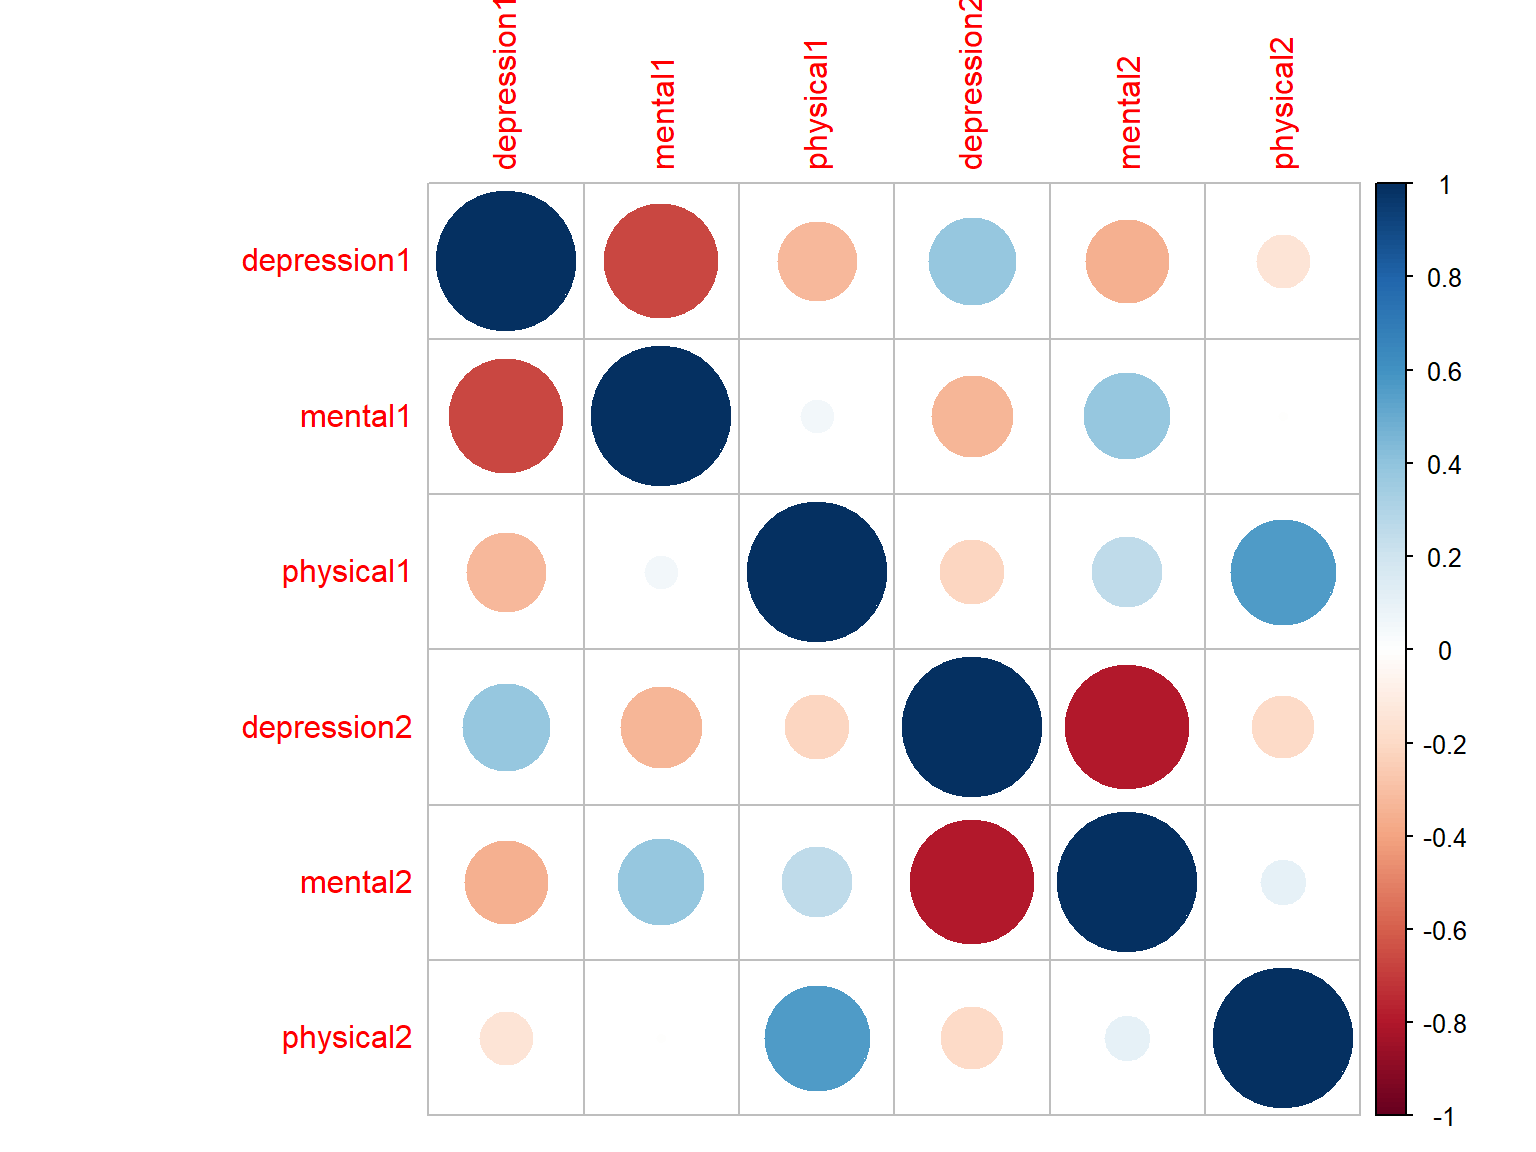
\includegraphics{rbook_files/figure-latex/corplot1-1} 

}

\caption{Correlation matrix plot with circles}\label{fig:corplot1}
\end{figure}

\begin{Shaded}
\begin{Highlighting}[]
\CommentTok{# Plot 2 with colors}
\KeywordTok{corrplot}\NormalTok{(cor_scores, }\DataTypeTok{method=}\StringTok{"color"}\NormalTok{)}
\end{Highlighting}
\end{Shaded}

\begin{figure}

{\centering 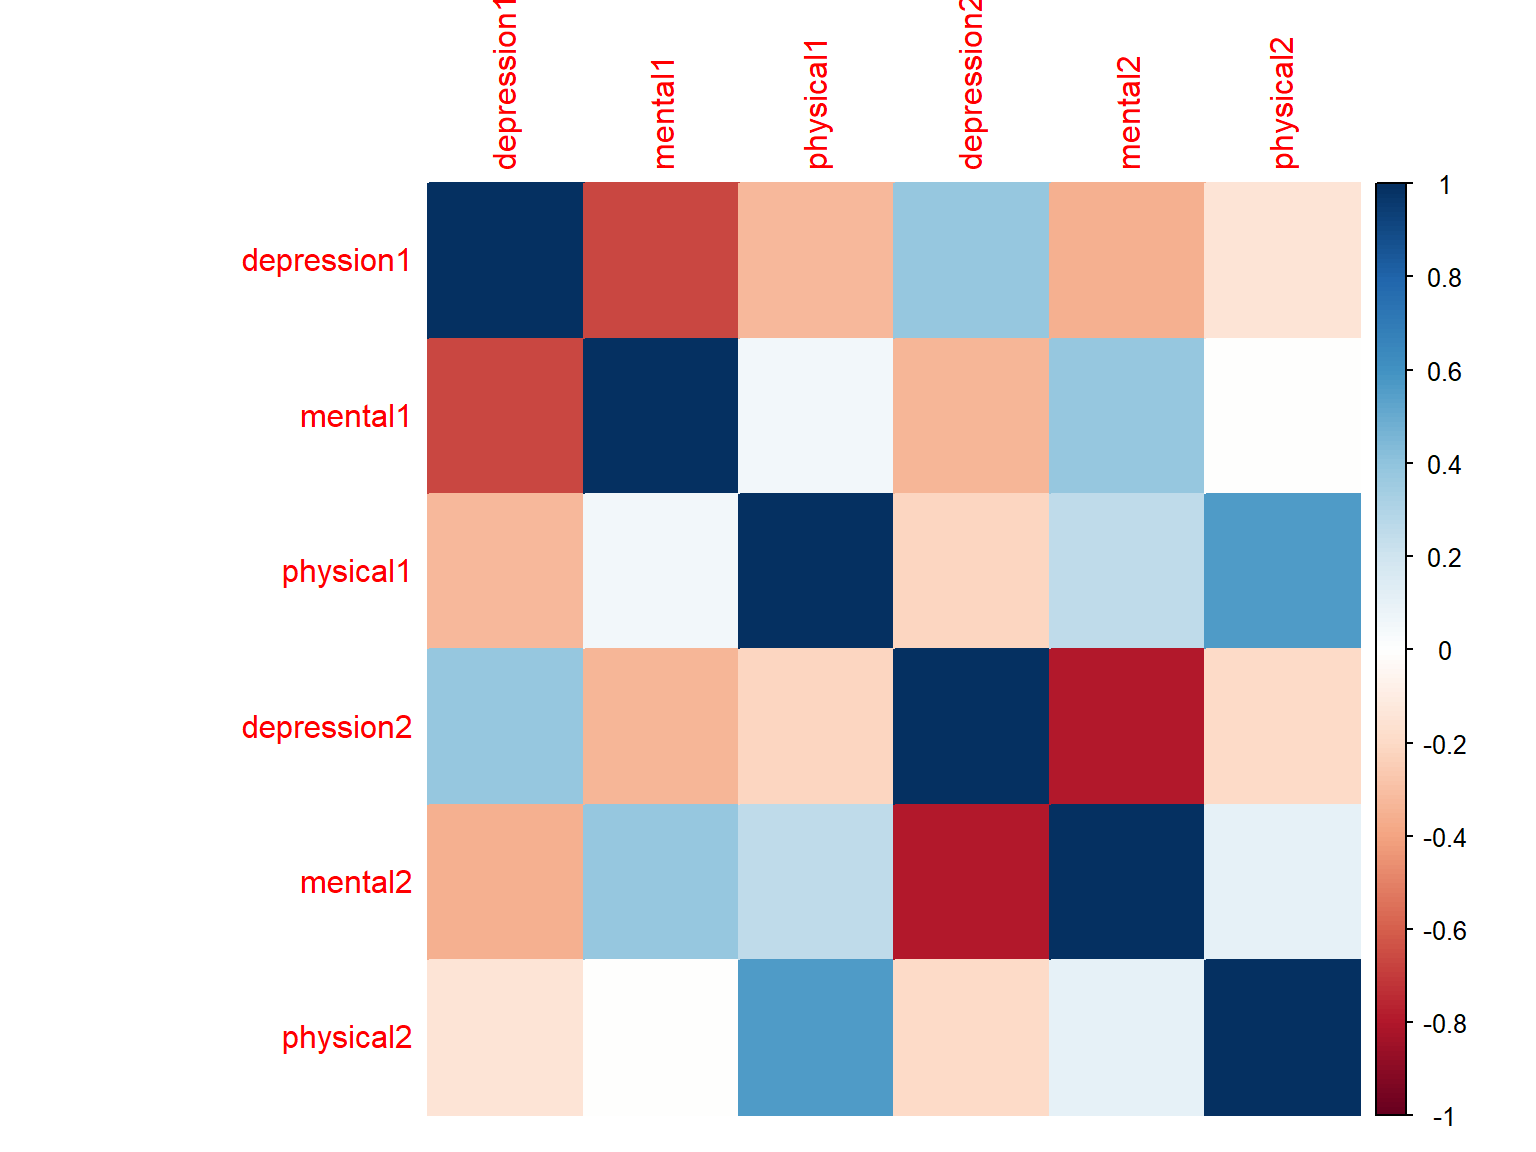
\includegraphics{rbook_files/figure-latex/corplot2-1} 

}

\caption{Correlation matrix plot with colours}\label{fig:corplot2}
\end{figure}

\begin{Shaded}
\begin{Highlighting}[]
\CommentTok{# Plot 3 with numbers}
\KeywordTok{corrplot}\NormalTok{(cor_scores, }\DataTypeTok{method=}\StringTok{"number"}\NormalTok{)}
\end{Highlighting}
\end{Shaded}

\begin{figure}

{\centering 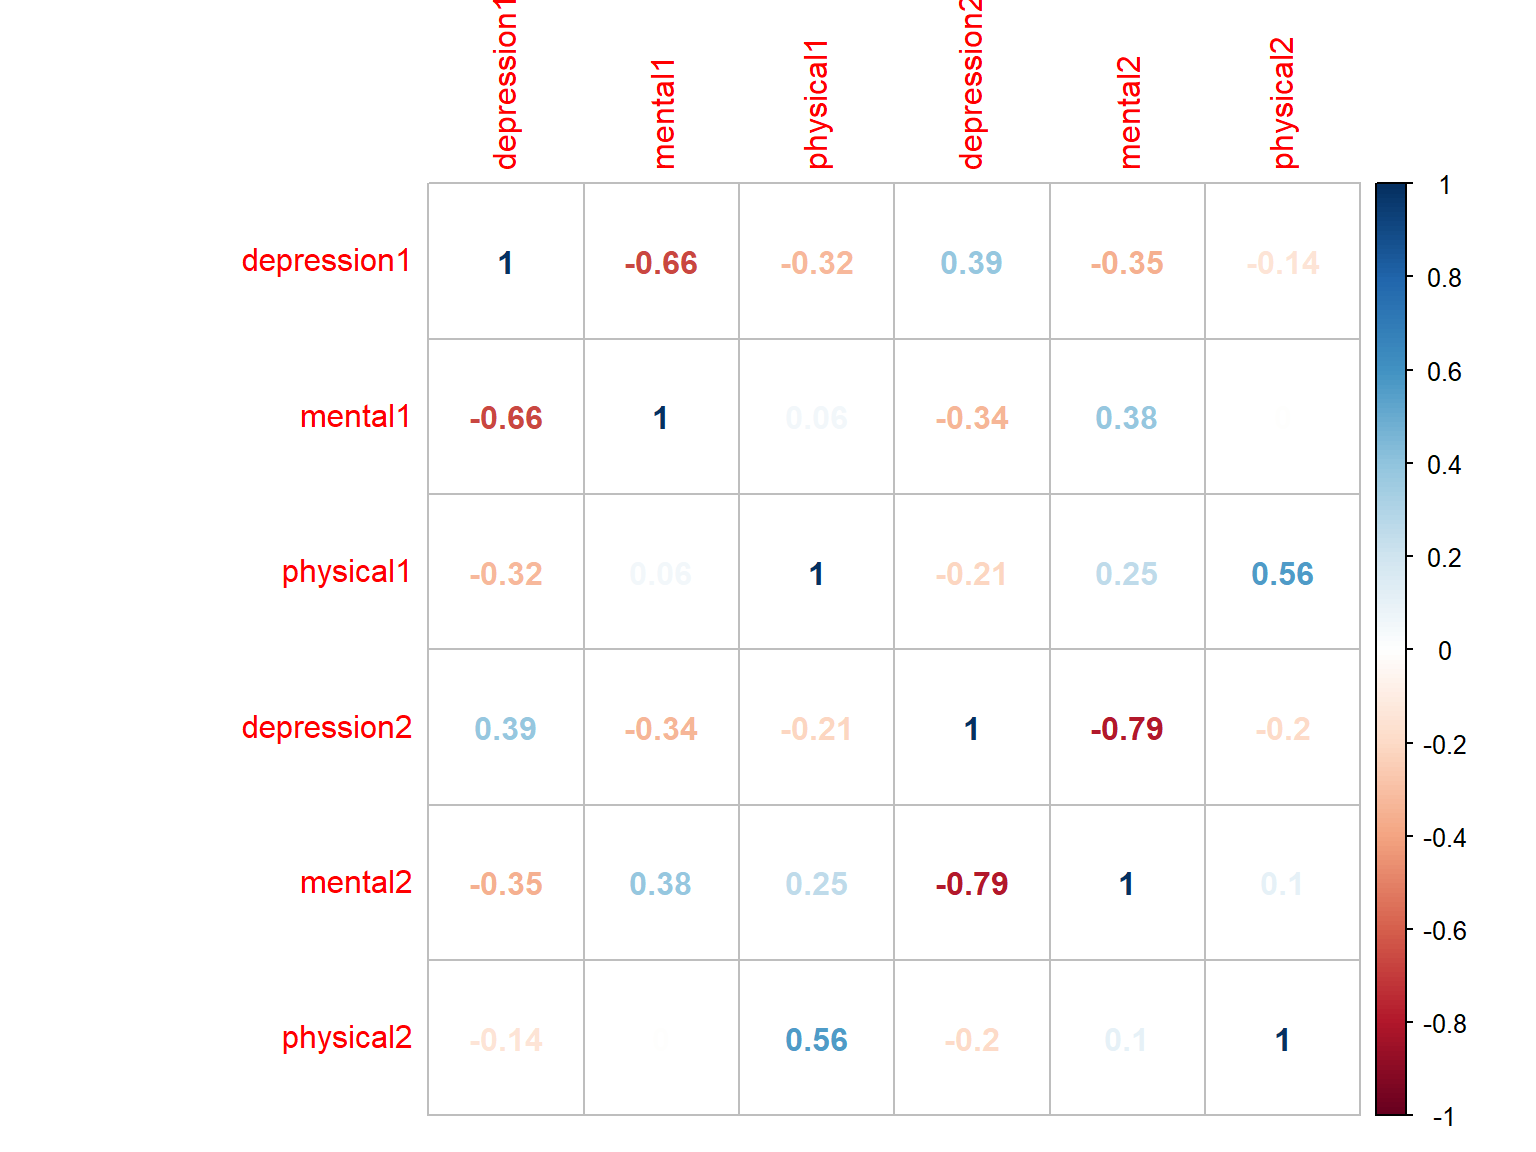
\includegraphics{rbook_files/figure-latex/corplot3-1} 

}

\caption{Correlation matrix plot with numbers}\label{fig:corplot3}
\end{figure}

\begin{Shaded}
\begin{Highlighting}[]
\CommentTok{# Plot 4 with circles + lower triangular}
\KeywordTok{corrplot}\NormalTok{(cor_scores, }\DataTypeTok{method=}\StringTok{"circle"}\NormalTok{, }\DataTypeTok{type=}\StringTok{"lower"}\NormalTok{)}
\end{Highlighting}
\end{Shaded}

\begin{figure}

{\centering 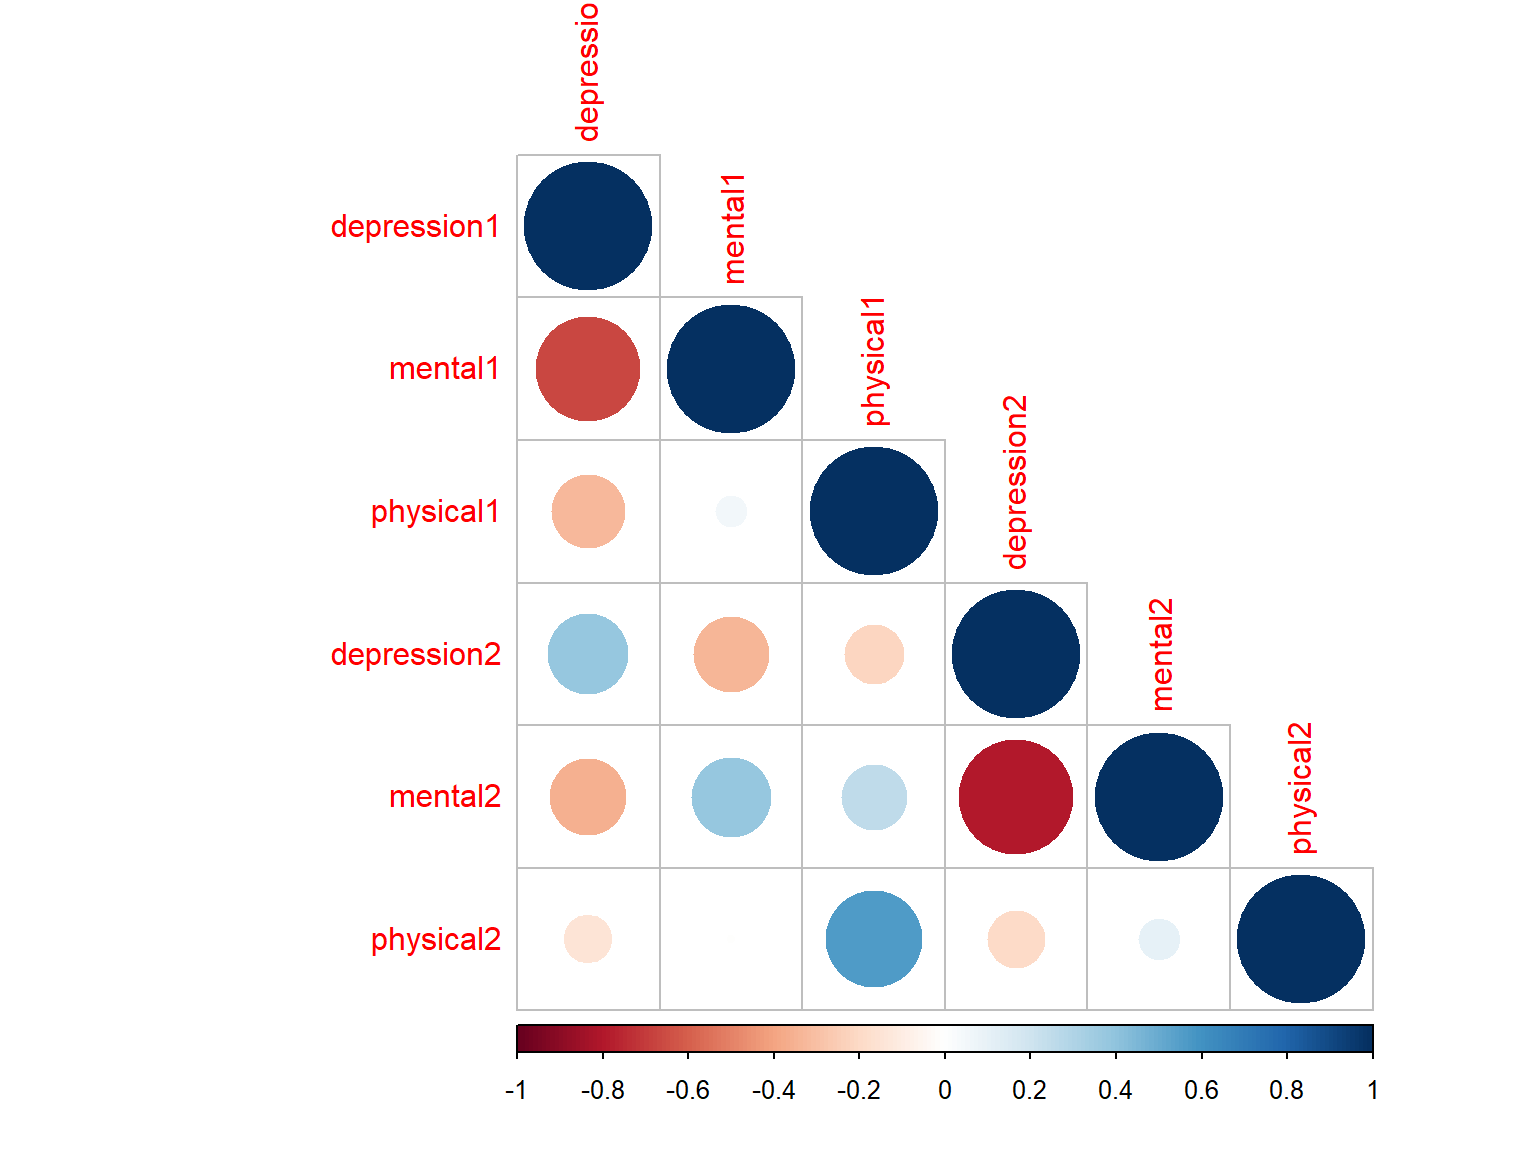
\includegraphics{rbook_files/figure-latex/corplot4-1} 

}

\caption{Correlation matrix plot with circle and lower triangle}\label{fig:corplot4}
\end{figure}

\begin{Shaded}
\begin{Highlighting}[]
\CommentTok{# Plot 5 with circles + lower triangular + ordered correlations}
\KeywordTok{corrplot}\NormalTok{(cor_scores, }\DataTypeTok{method=}\StringTok{"circle"}\NormalTok{, }\DataTypeTok{type=}\StringTok{"lower"}\NormalTok{, }\DataTypeTok{order=}\StringTok{"hclust"}\NormalTok{)}
\end{Highlighting}
\end{Shaded}

\begin{figure}

{\centering 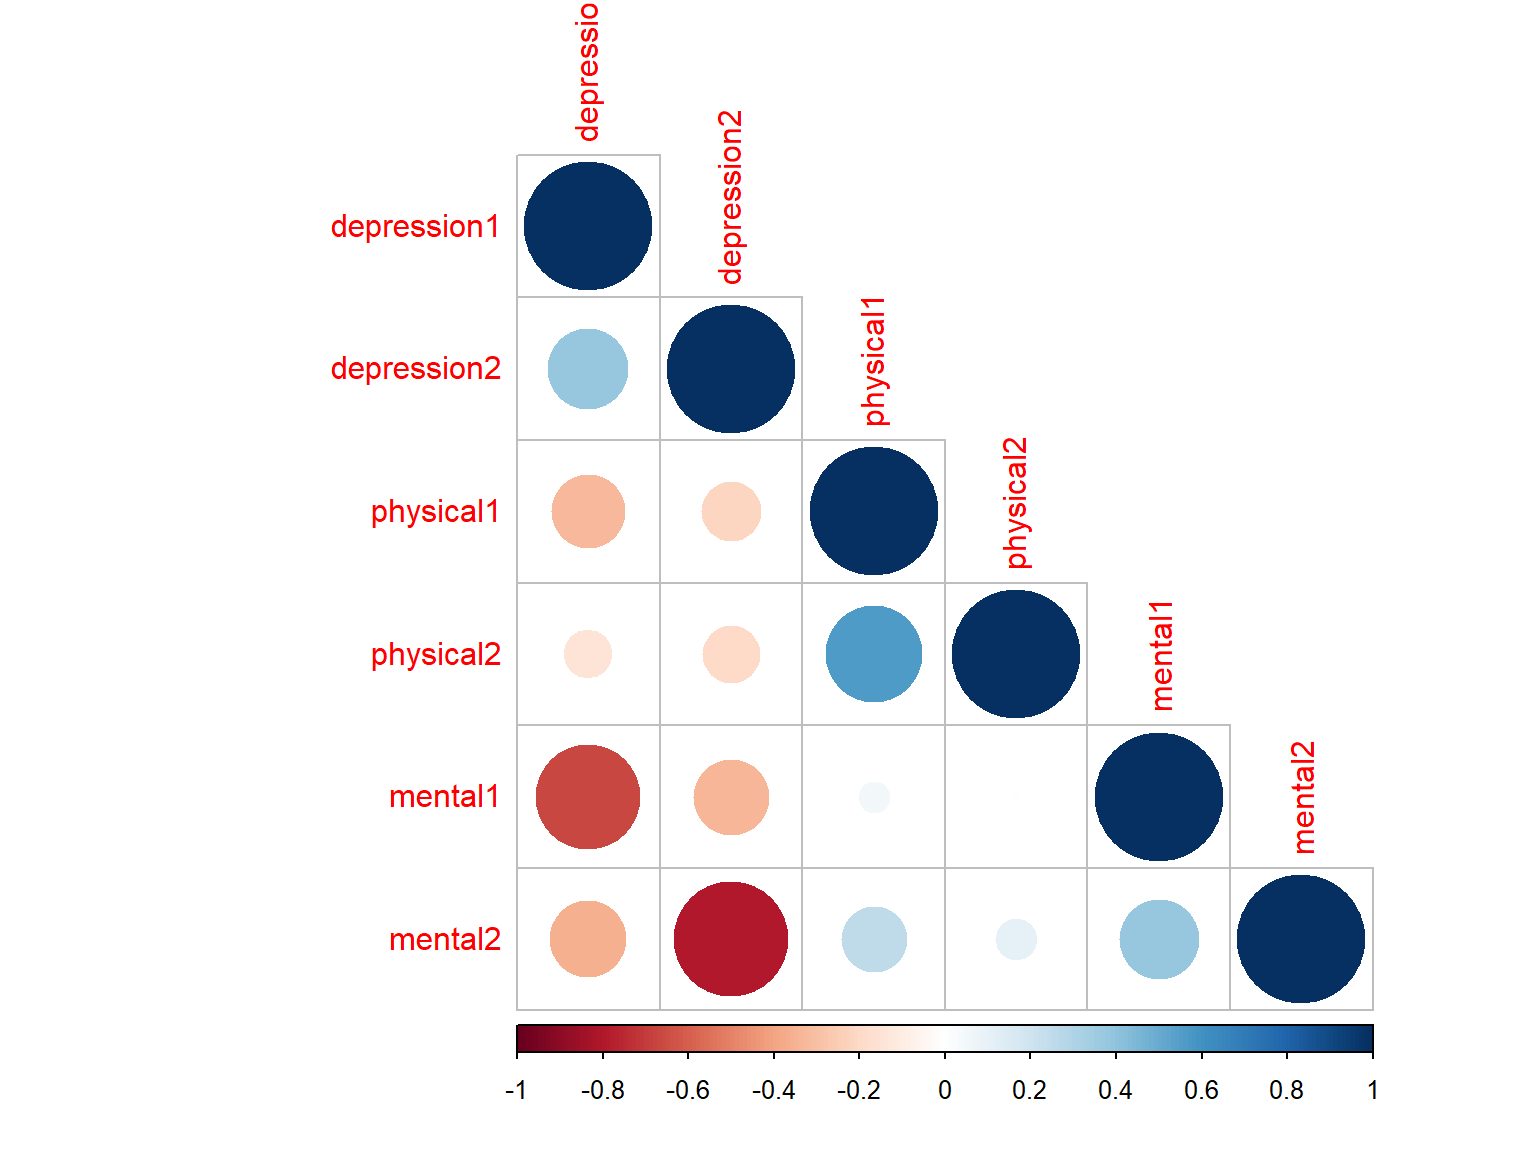
\includegraphics{rbook_files/figure-latex/corplot5-1} 

}

\caption{Correlation matrix plot with ordered correlations}\label{fig:corplot5}
\end{figure}

\hypertarget{simple-linear-regression}{%
\section{Simple Linear Regression}\label{simple-linear-regression}}

Linear regression is a standard tool that researchers rely on when analyzing the linear relationship between interval scale predictors (i.e., independent variables) and an interval scale outcome (i.e., dependent variable). In a simple linear regression model, we aim to fit the best linear line to the data based on a single predictor so that the sum of residuals is the smallest. This method is known as ``ordinaly least squares'' (OLS). Once the regression equation is computed, we can use it to make predictions for a new sample of observations.

If \(Y\) is the dependent variable (DV) and \(X\) is the predictor variable (IV), then the formula that describes our simple linear regression model is written like this:

\[ Y_i = b_1 X_i + b_0 + \epsilon_i\]

where \(b_1\) is the slope (the increase in \(Y\) for every one unit increase in \(X\)), \(b_0\) is the intercept (the value of \(Y\) when \(X=0\)), and \(\epsilon_i\) is the residual (the difference between the predicted values based on the regression model and the actual values of the dependent variable).

In \textbf{R}, there are many ways to run regression analyses. However, the simplest way to run a regression model in \textbf{R} is to use the \texttt{lm()} function that fits a linear model to a given dataset (see \texttt{?lm} in the console for the help page). Here are the typical elements of \texttt{lm()}:

\begin{itemize}
\tightlist
\item
  \texttt{formula}: A formula that specifies the regression model. This formula is of the form DV \textasciitilde{} IV.
\item
  \texttt{data}: The data frame containing the variables.
\end{itemize}

\hypertarget{example-4}{%
\subsection{Example}\label{example-4}}

Now let's see how regression works in \textbf{R}. We want to predict patients' mental scores at the baseline (i.e., \texttt{mental1}) using their depression scores at the baseline (i.e., \texttt{depression1}). To see how this relationship looks like, we can first take a look at the scatterplot as well as the correlation between the two variables.

\begin{Shaded}
\begin{Highlighting}[]
\KeywordTok{cor}\NormalTok{(medical}\OperatorTok{$}\NormalTok{depression1, medical}\OperatorTok{$}\NormalTok{mental1)}
\end{Highlighting}
\end{Shaded}

\begin{verbatim}
[1] -0.6629
\end{verbatim}

It seems that \(r = -.66\), indicating that there is a negative and moderately strong relationship between the two variables. Although we know that correlation does \textbf{NOT} mean causation, our knowledge or theory from the literature may suggest that these two variables are indeed associated with each other. So, we can move to the next step and plot these two variables in a scatterplot using the `\texttt{ggplot2} package (see \url{http://sape.inf.usi.ch/quick-reference/ggplot2/colour} for many colour options in \texttt{ggplot2}).

\begin{Shaded}
\begin{Highlighting}[]
\CommentTok{# Activate the ggplot2 first}
\KeywordTok{library}\NormalTok{(}\StringTok{"ggplot2"}\NormalTok{)}

\KeywordTok{ggplot}\NormalTok{(}\DataTypeTok{data =}\NormalTok{ medical, }
       \DataTypeTok{mapping =} \KeywordTok{aes}\NormalTok{(}\DataTypeTok{x =}\NormalTok{ depression1, }\DataTypeTok{y =}\NormalTok{ mental1)) }\OperatorTok{+}\StringTok{ }
\StringTok{  }\KeywordTok{geom_point}\NormalTok{(}\DataTypeTok{size =} \DecValTok{2}\NormalTok{, }\DataTypeTok{color =} \StringTok{"grey25"}\NormalTok{) }\OperatorTok{+}
\StringTok{  }\KeywordTok{geom_smooth}\NormalTok{(}\DataTypeTok{method =}\NormalTok{ lm, }\DataTypeTok{color =} \StringTok{"blue"}\NormalTok{, }\DataTypeTok{se =} \OtherTok{TRUE}\NormalTok{) }\OperatorTok{+}
\StringTok{  }\KeywordTok{labs}\NormalTok{(}\DataTypeTok{x =} \StringTok{"Depression scores"}\NormalTok{, }
       \DataTypeTok{y =} \StringTok{"Mental scores"}\NormalTok{,}
       \DataTypeTok{title =} \StringTok{"Scatterplot of depression and mental scores at the baseline"}\NormalTok{) }\OperatorTok{+}
\StringTok{  }\KeywordTok{theme_bw}\NormalTok{()}
\end{Highlighting}
\end{Shaded}

\begin{figure}

{\centering 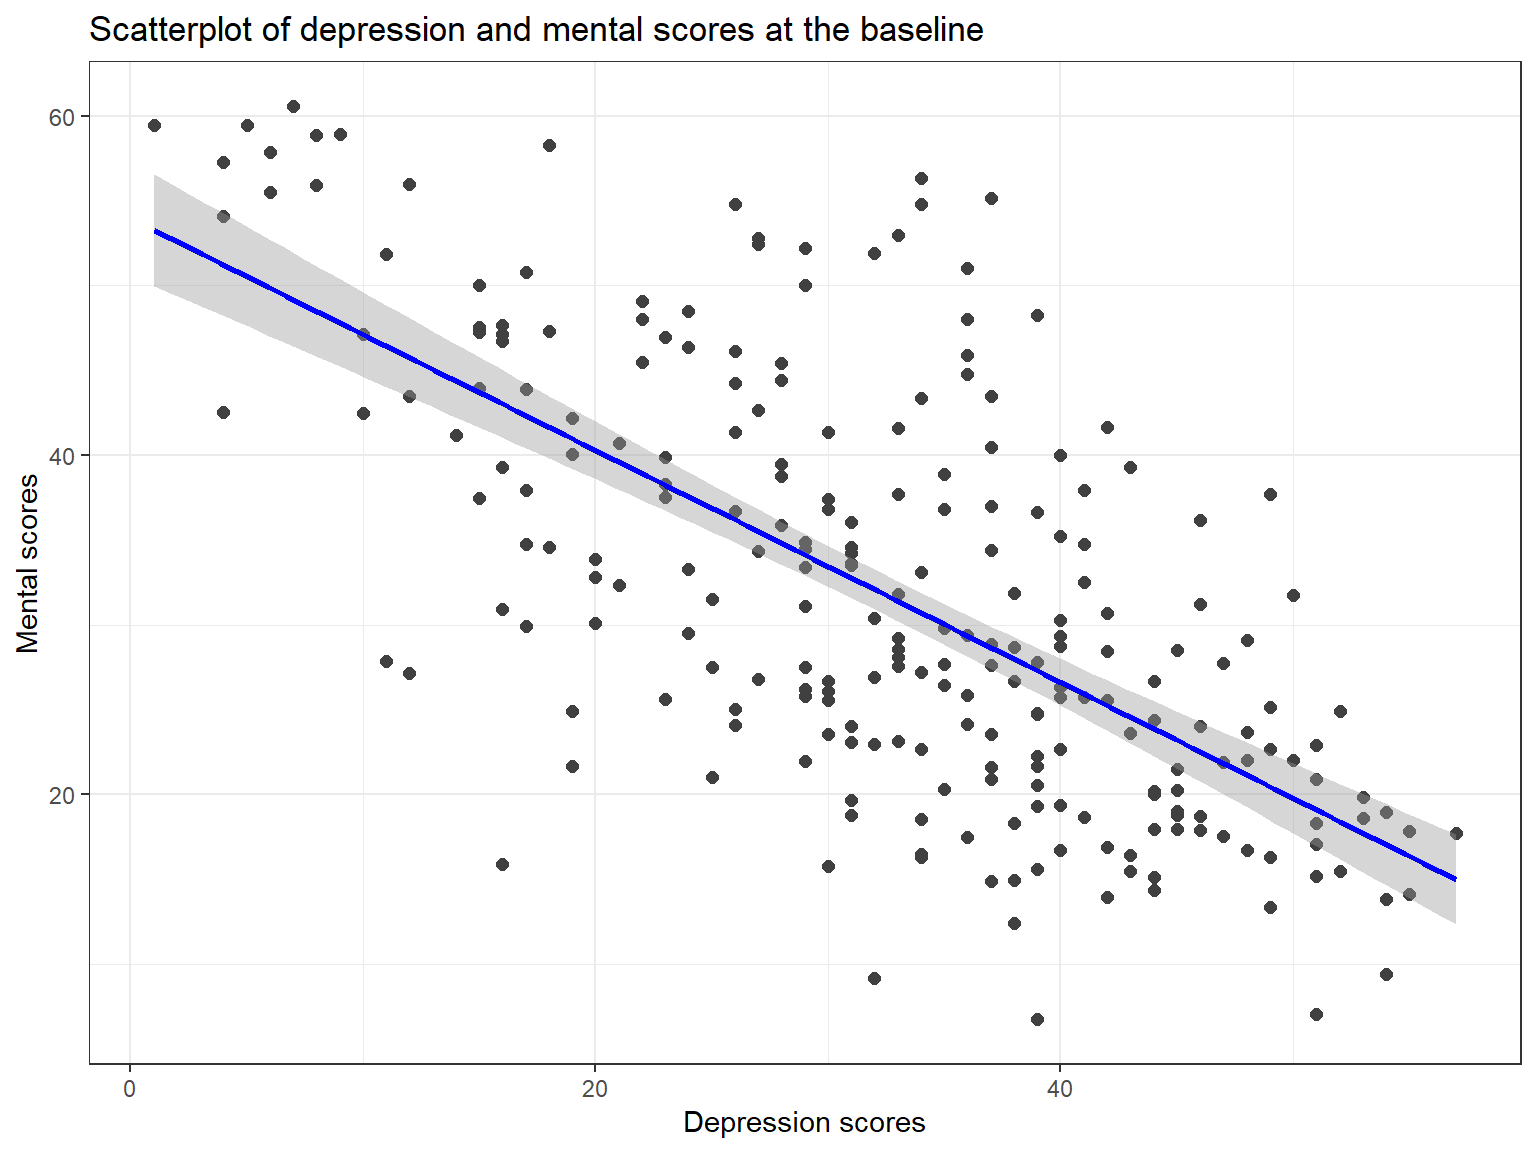
\includegraphics{rbook_files/figure-latex/ggscatter5-1} 

}

\caption{Scatterplot of depression and mental scores at the baseline}\label{fig:ggscatter5}
\end{figure}

The scatterplot also confirms that there is a negative relationship between the two variables. Now we can fit a simple linear regression model to the data to quantify this relationship.

\begin{Shaded}
\begin{Highlighting}[]
\CommentTok{# Set up the model and save it as model1}
\NormalTok{model1 <-}\StringTok{ }\KeywordTok{lm}\NormalTok{(mental1 }\OperatorTok{~}\StringTok{ }\NormalTok{depression1, }\DataTypeTok{data =}\NormalTok{ medical)}

\CommentTok{# Print basic model output}
\KeywordTok{print}\NormalTok{(model1)}
\end{Highlighting}
\end{Shaded}

\begin{verbatim}

Call:
lm(formula = mental1 ~ depression1, data = medical)

Coefficients:
(Intercept)  depression1  
     53.948       -0.683  
\end{verbatim}

\begin{Shaded}
\begin{Highlighting}[]
\CommentTok{# Print detailed summary of the model}
\KeywordTok{summary}\NormalTok{(model1)}
\end{Highlighting}
\end{Shaded}

\begin{verbatim}

Call:
lm(formula = mental1 ~ depression1, data = medical)

Residuals:
    Min      1Q  Median      3Q     Max 
-27.152  -6.993   0.039   5.853  26.464 

Coefficients:
            Estimate Std. Error t value Pr(>|t|)    
(Intercept)  53.9477     1.7173    31.4   <2e-16 ***
depression1  -0.6834     0.0494   -13.8   <2e-16 ***
---
Signif. codes:  0 '***' 0.001 '**' 0.01 '*' 0.05 '.' 0.1 ' ' 1

Residual standard error: 9.37 on 244 degrees of freedom
Multiple R-squared:  0.439, Adjusted R-squared:  0.437 
F-statistic:  191 on 1 and 244 DF,  p-value: <2e-16
\end{verbatim}

We can also use the \texttt{summ} function from the \texttt{jtools} package \citep{R-jtools} to print the output nicely.

\begin{Shaded}
\begin{Highlighting}[]
\CommentTok{# Install and activate the package}
\KeywordTok{install.packages}\NormalTok{(}\StringTok{"jtools"}\NormalTok{)}
\KeywordTok{library}\NormalTok{(}\StringTok{"jtools"}\NormalTok{)}

\CommentTok{# Print more organized output}
\KeywordTok{summ}\NormalTok{(model1)}
\end{Highlighting}
\end{Shaded}

\begin{table}[!h]
\centering
\begin{tabular}{lr}
\toprule
\rowcolor{gray!6}  Observations & 246\\
Dependent variable & mental1\\
\rowcolor{gray!6}  Type & OLS linear regression\\
\bottomrule
\end{tabular}
\end{table} \begin{table}[!h]
\centering
\begin{tabular}{lr}
\toprule
\rowcolor{gray!6}  F(1,244) & 191.27\\
R² & 0.44\\
\rowcolor{gray!6}  Adj. R² & 0.44\\
\bottomrule
\end{tabular}
\end{table} \begin{table}[!h]
\centering
\begin{threeparttable}
\begin{tabular}{lrrrr}
\toprule
  & Est. & S.E. & t val. & p\\
\midrule
\rowcolor{gray!6}  (Intercept) & 53.95 & 1.72 & 31.41 & 0.00\\
depression1 & -0.68 & 0.05 & -13.83 & 0.00\\
\bottomrule
\end{tabular}
\begin{tablenotes}
\item Standard errors: OLS
\end{tablenotes}
\end{threeparttable}
\end{table}

The output shows that our regression equation is:

\[\hat{mental1} = 53.9477 - 0.6834(depression1)\]
suggesting that one unit increase in the depression scores corresponds to -0.6834 points increase in the mental scores at the baseline.

\texttt{t\ val.} or \texttt{t\ value} in the outputs above indicate the individual \(t\) tests for testing whether intercept and slope are significantly different from zero; i.e., \(H_0 = b_0 = 0\) and \(H_0 = b_1 = 0\). The test for the intercept is not really interesting as we rarely care about whether or not the intercept is zero. However, for the slope, we want this test to be significant in order to conclude that the predictor is indeed useful for predicting the dependent variable. In our example, \(t = -13.8\) for the slope and its p-value is less than .001. This indicates that the slope was significantly different from zero (i.e., an important predictor in our model). In the output \texttt{***} shows the level of significance.

Another important information is \(R^2\), which indicates the proportion of the variance explained by the predictor (\texttt{depression1}) in the dependent variable (\texttt{mental1}). In our model, \(R^2 = 0.439\) -- which means \(43.9%
\) of the variance in the mental scores can be explained by the depression scores.

There are many guidelines for categorizing for interpreting R-squared values. Researchers often refers to Cohen's guidelines as shown below:

\begin{longtable}[]{@{}cc@{}}
\toprule
R-squared & Interpretation\tabularnewline
\midrule
\endhead
0.1 & Small\tabularnewline
0.09 & Moderate\tabularnewline
0.25 & Large\tabularnewline
\bottomrule
\end{longtable}

Using these guidelines, we can say that our model indicates a large-effect between the dependent and independent variable.

Finally, the output has additional information about the overall significance of the regression model: \(F(1, 244) = 191, p < .001\), suggesting that the model is statistically significant. This information may not be useful when we have a simple regression model because we already know that the predictor is significantly predicts the dependent variable. However, it will be more handy when we look at multiple regression where only some variables might be significant, not all of them.

\hypertarget{multiple-regression}{%
\section{Multiple Regression}\label{multiple-regression}}

The simple linear regression model that we have discussed up to this point assumes that there is a single predictor variable that we are interested in. However, in many (perhaps most) research projects, we actually have multiple predictors that we want to examine. Therefore, we can extend the linear regression framework to be able to include multiple predictors -- which is called \textbf{multiple regression}.

Multiple regression is conceptually very simple. All we do is to add more predictors into our regression equation. Let's suppose that we are interested in predicting the mental scores at the baseline (\texttt{mental1}) using both the depression scores at the baseline (\texttt{depression1}), the physical scores at the baseline (\texttt{physical1}), and sex (\texttt{sex}). Our new regression equation should look like this:

\[\hat{mental1} = b_0 + b_1(depression1) + b_2(physical1) + b_3(sex)\]

We would hope that the additional variables we include in the model will make our regression model more precise. In other words, we will be able to better predict the mental scores with the help of these predictors. The caveat is that these two variables should be correlated with the dependent variable (i.e., mental scores) but they should not be highly correlated with each other or the other predictor (i.e., depression scores). If this is the case, adding new variables would not bring additional value to the regression model. Rather, the model would have some redundant variables.

\hypertarget{example-5}{%
\subsection{Example}\label{example-5}}

Now let's see how this will look like in \textbf{R}.

\begin{Shaded}
\begin{Highlighting}[]
\CommentTok{# Add physical1 into the previous model}
\NormalTok{model2 <-}\StringTok{ }\KeywordTok{lm}\NormalTok{(mental1 }\OperatorTok{~}\StringTok{ }\NormalTok{depression1 }\OperatorTok{+}\StringTok{ }\NormalTok{physical1, }\DataTypeTok{data =}\NormalTok{ medical)}

\CommentTok{# Print detailed summary of the model}
\KeywordTok{summ}\NormalTok{(model2)}
\end{Highlighting}
\end{Shaded}

\begin{table}[!h]
\centering
\begin{tabular}{lr}
\toprule
\rowcolor{gray!6}  Observations & 246\\
Dependent variable & mental1\\
\rowcolor{gray!6}  Type & OLS linear regression\\
\bottomrule
\end{tabular}
\end{table} \begin{table}[!h]
\centering
\begin{tabular}{lr}
\toprule
\rowcolor{gray!6}  F(2,243) & 106.13\\
R² & 0.47\\
\rowcolor{gray!6}  Adj. R² & 0.46\\
\bottomrule
\end{tabular}
\end{table} \begin{table}[!h]
\centering
\begin{threeparttable}
\begin{tabular}{lrrrr}
\toprule
  & Est. & S.E. & t val. & p\\
\midrule
\rowcolor{gray!6}  (Intercept) & 64.92 & 3.56 & 18.23 & 0.00\\
depression1 & -0.74 & 0.05 & -14.52 & 0.00\\
\rowcolor{gray!6}  physical1 & -0.19 & 0.05 & -3.49 & 0.00\\
\bottomrule
\end{tabular}
\begin{tablenotes}
\item Standard errors: OLS
\end{tablenotes}
\end{threeparttable}
\end{table}

The output shows that our new regression equation is:

\[\hat{mental1} = 64.92 -0.74(depression1) -0.19(physical1)\]

Both predictors negatively predict the mental scores and they are statistically significant in the model. Our R-squared value increased to \(R^2=0.466\), suggesting that \(46.6%
\) of the variance can be explained by the two predictors that we have in the model.

By looking at the slopes for each predictor, we \textbf{cannot} tell which predictor plays a more important role in the prediction. Therefore, we need to see the standardized slopes -- which are directly comparable based on their magnitudes. Let's use the \texttt{plot\_summ} function from the \texttt{jtools} package to check these numbers visually:

\begin{Shaded}
\begin{Highlighting}[]
\KeywordTok{plot_summs}\NormalTok{(model2, }\DataTypeTok{scale =} \OtherTok{TRUE}\NormalTok{)}
\end{Highlighting}
\end{Shaded}

\begin{figure}

{\centering 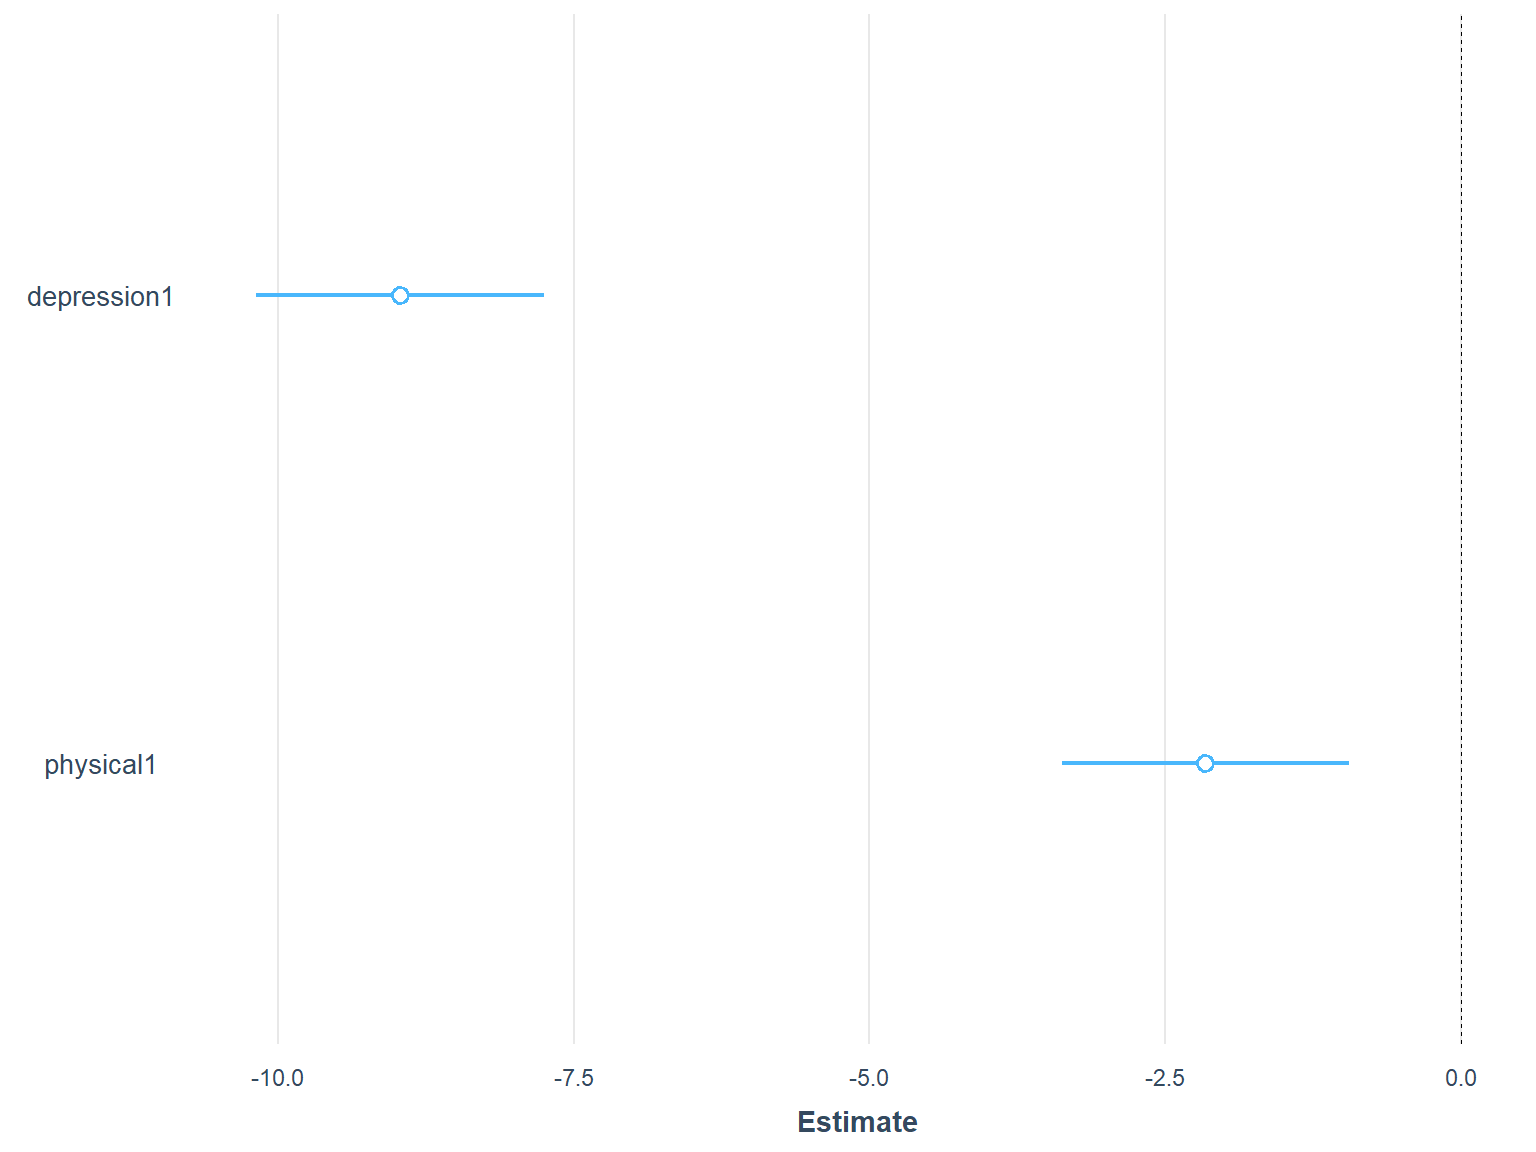
\includegraphics{rbook_files/figure-latex/regplot1-1} 

}

\caption{Standardized regression coefficients in Model 2}\label{fig:regplot1}
\end{figure}

In the plot, the circles in the middle show the location of the standardized slopes (i.e., regression coefficients) for both predictors and the line around the circles represent the confidence interval. We can see from Figure \ref{fig:regplot1} that the standardized slope for \texttt{depression1} is much larger (around -8.5) whereas the standardized slope for \texttt{physical1} is smaller (around -2). So, we could say that the \texttt{depression1} is a stronger predictor than \texttt{physical1} in predicting \texttt{mental1}.

Let's expand our model by adding \texttt{sex}. Because \texttt{sex} is a categorical variable, \textbf{R} will choose one level of this variable as the reference category and give the results for the other category. The default reference category is selected alphabetically. In the context of \texttt{sex}, the values are male and female. Because \textbf{f} alphabetically comes first, female will be selected as the reference category and we will see the results for male.

\begin{Shaded}
\begin{Highlighting}[]
\CommentTok{# Add physical1 into the previous model}
\NormalTok{model3 <-}\StringTok{ }\KeywordTok{lm}\NormalTok{(mental1 }\OperatorTok{~}\StringTok{ }\NormalTok{depression1 }\OperatorTok{+}\StringTok{ }\NormalTok{physical1 }\OperatorTok{+}\StringTok{ }\NormalTok{sex, }\DataTypeTok{data =}\NormalTok{ medical)}

\CommentTok{# Print detailed summary of the model}
\KeywordTok{summ}\NormalTok{(model3)}
\end{Highlighting}
\end{Shaded}

\begin{table}[!h]
\centering
\begin{tabular}{lr}
\toprule
\rowcolor{gray!6}  Observations & 246\\
Dependent variable & mental1\\
\rowcolor{gray!6}  Type & OLS linear regression\\
\bottomrule
\end{tabular}
\end{table} \begin{table}[!h]
\centering
\begin{tabular}{lr}
\toprule
\rowcolor{gray!6}  F(3,242) & 70.51\\
R² & 0.47\\
\rowcolor{gray!6}  Adj. R² & 0.46\\
\bottomrule
\end{tabular}
\end{table} \begin{table}[!h]
\centering
\begin{threeparttable}
\begin{tabular}{lrrrr}
\toprule
  & Est. & S.E. & t val. & p\\
\midrule
\rowcolor{gray!6}  (Intercept) & 64.64 & 3.73 & 17.33 & 0.00\\
depression1 & -0.74 & 0.05 & -14.33 & 0.00\\
\rowcolor{gray!6}  physical1 & -0.19 & 0.06 & -3.50 & 0.00\\
sexmale & 0.37 & 1.41 & 0.26 & 0.79\\
\bottomrule
\end{tabular}
\begin{tablenotes}
\item Standard errors: OLS
\end{tablenotes}
\end{threeparttable}
\end{table}

The output shows that the estimated slope for \texttt{sexmale} is 0.37; but this slope is not statistically significant as its p-value is 0.79. We could probably conclude that \texttt{sex} doesn't explain any further variance in the model and therefore we can remove it from the model to keep our regression model simple.

So far we tested three models: Model 1, Model 2, and Model 3. Because the models are nested within each other (i.e., we incrementally added new variables), we can make a model comparison to see if adding those additional predictors brought significant added-value to the models with more predictors. We will use the \texttt{anova} function in base \textbf{R} to accomplish this. This function doesn't necessarily run the same ANOVA as we discussed earlier. It will compare the models based on their R-squared values.

\begin{Shaded}
\begin{Highlighting}[]
\KeywordTok{anova}\NormalTok{(model1, model2, model3)}
\end{Highlighting}
\end{Shaded}

\begin{verbatim}
Analysis of Variance Table

Model 1: mental1 ~ depression1
Model 2: mental1 ~ depression1 + physical1
Model 3: mental1 ~ depression1 + physical1 + sex
  Res.Df   RSS Df Sum of Sq     F  Pr(>F)    
1    244 21411                               
2    243 20387  1      1024 12.16 0.00058 ***
3    242 20381  1         6  0.07 0.79390    
---
Signif. codes:  0 '***' 0.001 '**' 0.01 '*' 0.05 '.' 0.1 ' ' 1
\end{verbatim}

In the output, there are two comparisons:

\begin{itemize}
\tightlist
\item
  Model 1 vs.~Model 2
\item
  Model 2 vs.~Model 3
\end{itemize}

The comparison of Model 1 and Model 2 shows that \(F(1,1024)=12.16, p < .001\), suggesting that the larger model (Model 2) explains significantly more variance than the smaller model (Model 1).

The comparison of Model 2 and Model 3 shows that \(F(1,6)=0.07, p=.793\), suggesting that the larger model (Model 3) does \textbf{NOT} explain significantly more variance than the smaller model (Model 2), which confirms our earlier finding that \texttt{sex} did not bring additional value to the model.

We can also compare the three models visually.

\begin{Shaded}
\begin{Highlighting}[]
\KeywordTok{plot_summs}\NormalTok{(model1, model2, model3, }\DataTypeTok{scale =} \OtherTok{TRUE}\NormalTok{)}
\end{Highlighting}
\end{Shaded}

\begin{figure}

{\centering 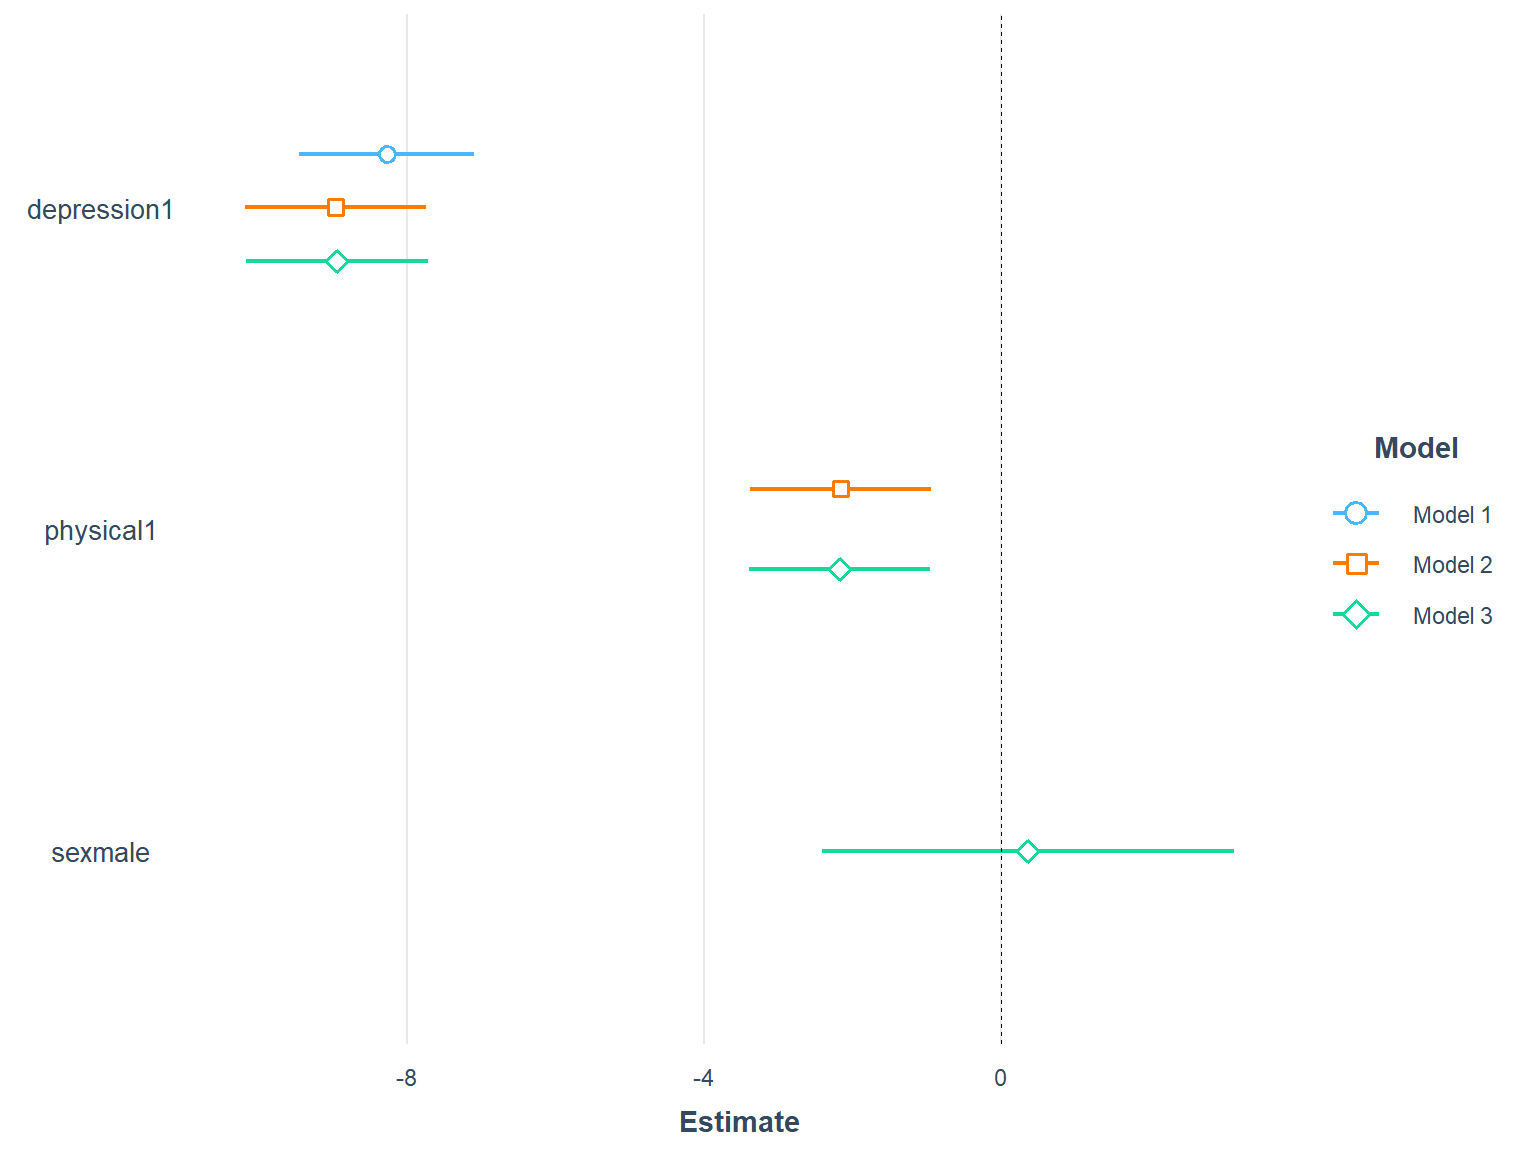
\includegraphics{rbook_files/figure-latex/regplot2-1} 

}

\caption{Comparison of three models}\label{fig:regplot2}
\end{figure}

\hypertarget{your-turn-9}{%
\subsection{Your Turn}\label{your-turn-9}}

Run a multiple regression model where your dependent variable will be \texttt{depression2} (i.e., depression scores after 6 months) and your predictors will be:

\begin{itemize}
\tightlist
\item
  \texttt{depression1} (i.e., depression scores at the baseline)
\item
  \texttt{treat1} (i.e., whether the patient received treatment)
\item
  \texttt{sex} (i.e., patients' sex)
\end{itemize}

The questions we can answer are:

\begin{enumerate}
\def\labelenumi{\arabic{enumi}.}
\tightlist
\item
  Which variables are significant?
\item
  Do we need all three predictors?
\item
  How is the R-squared value for the model?
\end{enumerate}

\bibliography{book.bib,packages.bib}


\end{document}
